\documentclass[11pt,a4paper,openany]{book}

% ============================================================
%  PAQUETS
% ============================================================
\usepackage[utf8]{inputenc}
\usepackage[T1]{fontenc}
\usepackage[french]{babel}

% --- Typographie & mise en page ---
\usepackage{geometry}
\geometry{a4paper, top=2.5cm, bottom=2.5cm, left=2cm, right=2cm, headheight=17.3pt}

\usepackage{microtype}          % Justification micro-typographique

% --- Police principale : Helvetica/Arial (universellement disponible) ---
\usepackage{lmodern}
\usepackage{helvet}
\renewcommand{\familydefault}{\sfdefault}  % Sans-serif par défaut

% --- Couleurs ---
\usepackage[table,dvipsnames]{xcolor}
\definecolor{primary}{gray}{0}           % Noir
\definecolor{accent}{gray}{0}            % Noir
\definecolor{lightgray}{gray}{0.96}      % Gris très clair
\definecolor{midgray}{gray}{0.75}        % Gris moyen
\definecolor{darktext}{gray}{0.1}        % Gris foncé
\definecolor{hfcolor}{gray}{0.3}         % Gris HF
\definecolor{bfcolor}{gray}{0.45}        % Gris BF

% --- En-têtes et pieds de page ---
\usepackage{fancyhdr}
\pagestyle{fancy}
\fancyhf{}
\renewcommand{\headrulewidth}{0pt}       % On gère le filet manuellement

% En-tête : filet coloré + titre du chapitre (à gauche) + numéro de page (à droite)
\fancyhead[L]{%
  \color{primary}\small\scshape\leftmark%
}
\fancyhead[R]{%
  \color{accent}\small\textbf{\thepage}%
}
% Ligne de séparation sous l'en-tête
\renewcommand{\headrule}{%
  {\color{accent}\hrule width\headwidth height 1.5pt}%
  \vspace{1pt}%
  {\color{midgray}\hrule width\headwidth height 0.4pt}%
}
\renewcommand{\headrulewidth}{1.5pt}

% Pas de pied de page
\fancyfoot{}

% Style de la page de garde (pas d'en-tête)
\fancypagestyle{plain}{%
  \fancyhf{}%
  \fancyfoot{}%
  \renewcommand{\headrulewidth}{0pt}%
}

% --- Chapitres et sections ---
\usepackage{titlesec}

% Format du titre de chapitre
\titleformat{\chapter}[display]
  {\color{primary}\bfseries\LARGE}
  {\color{accent}\normalfont\large\MakeUppercase{\chaptertitlename}\ \thechapter}
  {0.5em}
  {}

\titlespacing*{\chapter}{0pt}{-10pt}{30pt}

% Format des sections
\titleformat{\section}
  {\color{primary}\bfseries\large}
  {\color{accent}\thesection}
  {0.8em}
  {}
\titlespacing*{\section}{0pt}{0.9em}{0.5em}

\titleformat{\subsection}
  {\color{darktext}\bfseries\normalsize}
  {\color{accent}\thesubsection}
  {0.6em}
  {}
\titlespacing*{\subsection}{0pt}{0.7em}{0.4em}

% --- Tableaux ---
\usepackage{booktabs}
\usepackage{tabularx}
\usepackage{multirow}
\usepackage{array}
\newcolumntype{L}[1]{>{\raggedright\arraybackslash}p{#1}}
\newcolumntype{C}[1]{>{\centering\arraybackslash}p{#1}}

% Style de tableau avec fond alterné
\usepackage{colortbl}
\newcommand{\tableheadcolor}{\rowcolor{lightgray}}
\newcommand{\tablerowodd}{}

% Affichage "moyenne ± écart-type" (multi-seed) : \res{moyenne}{std}
\newcommand{\res}[2]{#1\,{\footnotesize$\pm$\,#2}}

% --- Boîtes et encadrés ---
\usepackage{tcolorbox}
\tcbuselibrary{skins, breakable}

% Boîte "Hypothèse"
\newtcolorbox{hypothesebox}[1][]{
  enhanced, breakable,
  colback=white, colframe=midgray,
  fonttitle=\bfseries\small\color{primary},
  title={#1},
  left=6pt, right=6pt, top=4pt, bottom=4pt,
  arc=3pt
}

% Boîte "Décision"
\newtcolorbox{decisionbox}{
  enhanced,
  colback=white, colframe=midgray,
  fontupper=\small,
  left=8pt, right=8pt, top=6pt, bottom=6pt,
  arc=4pt
}

% --- Listes ---
\usepackage{enumitem}
\setlist[itemize]{leftmargin=1.5em, itemsep=2pt, topsep=4pt}
\setlist[enumerate]{leftmargin=1.5em, itemsep=2pt, topsep=4pt}

% --- Graphiques / schémas ---
\usepackage{graphicx}
\usepackage{tikz}
\usetikzlibrary{shapes.geometric, arrows.meta, positioning, fit, backgrounds, calc}
\tikzset{every picture/.style={font=\footnotesize}}

% --- Symboles mathématiques ---
\usepackage{amsmath}
\usepackage{amssymb}

% --- Hyperliens ---
\usepackage{hyperref}
\hypersetup{
  colorlinks=true,
  linkcolor=accent,
  urlcolor=accent,
  citecolor=accent,
  pdftitle={Projet PF22 - Approche Multi-Fidélité},
  pdfauthor={Ivann Vasic}
}

% --- Espacement ---
\usepackage{setspace}
\setstretch{1.25}
\setlength{\parskip}{6pt}
\setlength{\parindent}{0pt}
\setlength{\textfloatsep}{10pt plus 2pt minus 2pt}
\setlength{\intextsep}{8pt plus 2pt minus 2pt}
\setlength{\floatsep}{8pt plus 2pt minus 2pt}

% ============================================================
%  MÉTADONNÉES
% ============================================================
\title{}
\author{}
\date{}

% ============================================================
%  DOCUMENT
% ============================================================
\begin{document}

% ============================================================
%  PAGE DE GARDE
% ============================================================
\thispagestyle{empty}
\begin{center}
\vspace*{2cm}
{\Large\textbf{UNIVERSITÉ DE TECHNOLOGIE DE BELFORT-MONTBÉLIARD}}\\[0.8em]
{\normalsize Projet PF22}\\[2.4cm]

{\large\textbf{RAPPORT DE PROJET}}\\[1em]
{\LARGE\textbf{Réduction des Coûts d'Apprentissage}}\\[0.35em]
{\LARGE\textbf{par Approche Multi-Fidélité}}\\[1.8cm]

\begin{minipage}{0.82\textwidth}
\centering
\normalsize
Ce projet explore la possibilité de réduire drastiquement les coûts
de constitution d'un jeu de données en combinant une faible proportion
d'images \textbf{Haute Fidélité} avec une grande majorité d'images
\textbf{Basse Fidélité} acquises à moindre coût.
\end{minipage}\\[2.2cm]

\rule{0.72\textwidth}{0.4pt}\\[0.8em]
\begin{tabular}{rl}
\textbf{Auteur :} & Ivann Vasic \\
\textbf{Période :} & Mars -- Juin 2026 \\
\textbf{Cadre :} & Projet PF22 --- UTBM \\
\end{tabular}
\end{center}

\newpage

% ============================================================
%  RÉSUMÉ
% ============================================================
\thispagestyle{empty}
\vspace*{1.5cm}
{\color{primary}\LARGE\bfseries Résumé}\\[0.5em]
{\color{accent}\rule{\linewidth}{1.5pt}}\\[0.3em]
{\color{midgray}\rule{\linewidth}{0.4pt}}
\vspace{0.8em}

L'entraînement de modèles d'apprentissage profond performants nécessite traditionnellement de vastes ensembles de données de haute qualité, dont l'acquisition et l'annotation s'avèrent souvent coûteuses en temps et en ressources. Ce projet explore une approche alternative : \textbf{l'apprentissage multi-fidélité}.

L'objectif est de démontrer qu'il est possible de réduire drastiquement les coûts de constitution d'un jeu de données en combinant une faible proportion d'images de \textbf{Haute Fidélité (HF)} avec une grande majorité d'images dégradées acquises à moindre coût (\textbf{Basse Fidélité - BF}), tout en maximisant la performance sur le domaine HF.

Sur la base d'un pipeline de dégradation contrôlé, d'un modèle de coût à trois métriques et de trois modèles de référence, \textbf{quatre stratégies multi-fidélité} ont été conçues et comparées : Transfer Learning séquentiel, Co-training pondéré, Curriculum Learning progressif et Elastic Weight Consolidation (EWC). Chacune a été \textbf{optimisée par Optuna} et évaluée selon un protocole rigoureux — \textbf{trois jeux de données} (Animals-10, Imagewoof, Intel) et \textbf{trois graines aléatoires} (résultats en moyenne $\pm$ écart-type) — complété par des analyses de robustesse à la dégradation et de sensibilité au ratio de coût.

Les résultats montrent que les stratégies séquentielles guidées (Transfer Learning et surtout \textbf{EWC}) atteignent la meilleure précision HF, \textbf{dépassant le mélange naïf coûteux tout en divisant le coût total par environ deux}, et ce de façon cohérente sur les trois datasets. L'objectif est donc atteint : des données bon marché et imparfaites, bien exploitées, deviennent un véritable levier de performance plutôt qu'un compromis dégradé.

\vspace{1.5em}
\begin{tcolorbox}[
  enhanced,
  colback=white,
  colframe=midgray,
  arc=4pt,
  left=8pt,
  right=8pt,
  top=8pt,
  bottom=8pt,
  boxrule=0.8pt
]
\textbf{Mots-clés :} Apprentissage profond $\cdot$ Multi-fidélité $\cdot$ CNN $\cdot$ ResNet-18 $\cdot$
Dégradation d'image $\cdot$ Optimisation des coûts $\cdot$ Domain Shift $\cdot$
Transfer learning $\cdot$ Curriculum learning $\cdot$ EWC $\cdot$ Optuna $\cdot$
Animals-10 $\cdot$ Imagewoof $\cdot$ Intel
\end{tcolorbox}

\newpage

% ============================================================
%  TABLE DES MATIÈRES
% ============================================================
\tableofcontents

\newpage

% ============================================================
%  TABLE DES FIGURES
% ============================================================
\addcontentsline{toc}{chapter}{Table des figures}
\listoffigures

\newpage

% ============================================================
%  LISTE DES ACRONYMES
% ============================================================
\thispagestyle{empty}
\addcontentsline{toc}{chapter}{Liste des acronymes}
{\color{primary}\LARGE\bfseries Liste des acronymes}\\[0.5em]
{\color{accent}\rule{\linewidth}{1.5pt}}\\[0.3em]
{\color{midgray}\rule{\linewidth}{0.4pt}}
\vspace{1em}

\renewcommand{\arraystretch}{1.35}
\begin{tabularx}{\linewidth}{L{2.6cm} X}
  \arrayrulecolor{midgray}
  \toprule
  \tableheadcolor
  \textbf{Sigle} & \textbf{Signification} \\
  \midrule
  \tablerowodd
  HF & Haute Fidélité (images propres, haute résolution, coûteuses) \\
  BF & Basse Fidélité (images dégradées, bon marché) \\
  \tablerowodd
  CA & Unité de coût d'acquisition (coût normalisé des données) \\
  BL & \textit{Baseline} (modèle de référence : BL 1 Premium, BL 2 Low-Cost, BL 3 Mixte) \\
  \tablerowodd
  S1--S4 & Stratégies multi-fidélité 1 à 4 (Transfer, Co-training, Curriculum, EWC) \\
  CNN & \textit{Convolutional Neural Network} (réseau de neurones convolutif) \\
  \tablerowodd
  ResNet & \textit{Residual Network} (architecture à connexions résiduelles) \\
  EWC & \textit{Elastic Weight Consolidation} (consolidation des poids par pénalité de Fisher) \\
  \tablerowodd
  HPO & \textit{Hyperparameter Optimization} (optimisation d'hyperparamètres) \\
  TPE & \textit{Tree-structured Parzen Estimator} (échantillonneur bayésien d'Optuna) \\
  \tablerowodd
  LR & \textit{Learning Rate} (taux d'apprentissage) \\
  AMP & \textit{Automatic Mixed Precision} (précision mixte automatique, FP16/FP32) \\
  \tablerowodd
  GPU & \textit{Graphics Processing Unit} (processeur graphique de calcul) \\
  JPEG & Format de compression d'image avec pertes (qualité $q$) \\
  \tablerowodd
  $\sigma$ & Écart-type du bruit gaussien appliqué dans la dégradation \\
  \bottomrule
\end{tabularx}

\newpage

% ============================================================
%  INTRODUCTION
% ============================================================
\chapter{Introduction}

\section{Contexte}

L'apprentissage profond a transformé la vision par ordinateur, mais sa performance reste fortement conditionnée par la \textbf{quantité et la qualité des données annotées}. Or, dans la plupart des contextes industriels et scientifiques, l'acquisition de données de \textbf{haute fidélité} (images haute résolution, capteurs coûteux, annotation par des experts) est lente et onéreuse. À l'inverse, il est souvent possible d'obtenir en abondance des données de \textbf{basse fidélité} : images dégradées, faible résolution, capteurs bon marché, étiquetage automatique ou collecté sur le web.

Ce déséquilibre est précisément le cadre de l'\textbf{apprentissage multi-fidélité}~\cite{kennedy2000,multifidelity} : combiner un petit volume de données précises et coûteuses (HF) avec un grand volume de données approximatives et bon marché (BF), afin d'atteindre la meilleure performance possible \emph{au meilleur coût}. La question centrale n'est plus seulement « quelle précision peut-on atteindre ? », mais « \textbf{quelle précision peut-on atteindre pour un budget d'acquisition donné ?} ».

\section{Problématique}

Mélanger naïvement des données HF et BF pose deux difficultés. D'une part, les données BF introduisent un \textbf{décalage de domaine} (\textit{domain shift}) : un modèle entraîné sur des images nettes s'effondre sur des images bruitées, et réciproquement. D'autre part, le coût n'est pas une grandeur unique : le coût d'\textbf{acquisition} des données (payé une fois) et le coût de \textbf{calcul} de l'entraînement obéissent à des logiques différentes et doivent être distingués pour comparer équitablement les approches.

La problématique de ce travail se formule ainsi :

\begin{quote}
\itshape Comment exploiter un faible volume de données haute fidélité, conjointement à un grand volume de données basse fidélité bon marché, pour maximiser la performance d'un réseau de neurones sur le domaine haute fidélité, tout en minimisant le coût d'acquisition ?
\end{quote}

L'\textbf{objectif est explicitement orienté HF} : la métrique cible prioritaire est la précision sur des données propres (Test HF), les données BF n'étant qu'un levier économique pour y parvenir.

\section{Démarche et contributions}

Pour répondre à cette question de manière rigoureuse, ce travail met en place un protocole expérimental complet et reproductible, dont les principales contributions sont :

\begin{itemize}
  \item un \textbf{pipeline de dégradation contrôlé et déterministe} (sous-échantillonnage, bruit gaussien, compression JPEG) qui simule des données BF à partir de données HF, appliqué à la volée ;
  \item un \textbf{modèle de coût explicite} distinguant trois métriques (coût d'acquisition, coût de calcul, coût total pondéré), fondé sur un coût unitaire fonction de la résolution ;
  \item trois \textbf{modèles de référence} (Premium HF, Low-Cost BF, Mixte) servant de bornes de comparaison ;
  \item quatre \textbf{stratégies multi-fidélité} — Transfer Learning séquentiel, Co-training pondéré, Curriculum Learning progressif et Elastic Weight Consolidation (EWC) — toutes orientées objectif HF ;
  \item une \textbf{optimisation des hyperparamètres} de chaque stratégie par Optuna ;
  \item une \textbf{validation de robustesse} : multi-graines (moyenne $\pm$ écart-type), triple jeu de données (Animals-10, Imagewoof, Intel), analyse de robustesse face à la dégradation et analyse de sensibilité au ratio de coût.
\end{itemize}

L'ensemble a été développé sous une architecture hybride VS~Code/Colab pour le prototypage, puis exécuté à grande échelle sur un serveur GPU NVIDIA V100S.

\section{Organisation du rapport}

Le rapport débute par les \textbf{notions préliminaires} d'apprentissage profond nécessaires à la lecture. Il décrit ensuite la \textbf{fondation expérimentale} (environnement, jeux de données, pipeline de dégradation, modèle de coût), puis les \textbf{modèles de référence}. Le cœur du travail présente les \textbf{quatre stratégies multi-fidélité}, suivies de leur \textbf{optimisation par Optuna}. Deux chapitres d'\textbf{analyses transversales} (robustesse face à la dégradation, sensibilité au ratio de coût) précèdent une \textbf{synthèse globale} comparant toutes les approches, puis la \textbf{conclusion et les perspectives}. Les leviers d'amélioration identifiés pour chaque stratégie sont regroupés en \textbf{annexe}.


% ============================================================
%  CHAPITRE — NOTIONS PRÉLIMINAIRES
% ============================================================
\chapter{Notions Préliminaires}

Ce chapitre présente les concepts fondamentaux nécessaires à la compréhension du projet. Le lecteur familier avec l'apprentissage profond peut passer directement au Chapitre~2.

% ---- 0.1 Réseaux de neurones ----
\section{Les réseaux de neurones artificiels}

Un réseau de neurones artificiel est un système de calcul inspiré du cerveau biologique. Il est constitué d'unités élémentaires, les \textbf{neurones}, organisées en \textbf{couches} successives. Chaque neurone reçoit des signaux numériques en entrée, les combine linéairement, puis applique une \textbf{fonction d'activation} non-linéaire avant de transmettre le résultat à la couche suivante.

\vspace{0.8em}
\begin{center}
\begin{tikzpicture}[
  font=\small,
  neuron/.style={circle, draw=midgray, fill=lightgray, minimum size=0.72cm, inner sep=0pt},
  hneuron/.style={circle, draw=hfcolor, fill=hfcolor!15, minimum size=0.72cm, inner sep=0pt},
  oneuron/.style={circle, draw=accent, fill=accent!10, minimum size=0.72cm, inner sep=0pt},
  arrow/.style={-Stealth, color=midgray, thin}
]
  % Couche d'entrée
  \foreach \i in {1,2,3,4} {
    \node[neuron] (i\i) at (0, -\i*1.1) {};
  }
  \node[above=0.2cm of i1, font=\footnotesize\bfseries, color=primary] {Entrée};

  % Couche cachée 1
  \foreach \i in {1,2,3,4,5} {
    \node[hneuron] (h1\i) at (2.2, -\i*1.1+0.55) {};
  }
  \node[above=0.2cm of h11, font=\footnotesize\bfseries, color=hfcolor] {Couche cachée};

  % Couche cachée 2
  \foreach \i in {1,2,3,4,5} {
    \node[hneuron] (h2\i) at (4.4, -\i*1.1+0.55) {};
  }

  % Couche de sortie
  \foreach \i in {1,2,3} {
    \node[oneuron] (o\i) at (6.6, -\i*1.1-0.55) {};
  }
  \node[above=0.2cm of o1, font=\footnotesize\bfseries, color=accent] {Sortie};

  % Connexions entrée → h1
  \foreach \i in {1,2,3,4} {
    \foreach \j in {1,2,3,4,5} {
      \draw[arrow] (i\i) -- (h1\j);
    }
  }
  % Connexions h1 → h2
  \foreach \i in {1,2,3,4,5} {
    \foreach \j in {1,2,3,4,5} {
      \draw[arrow] (h1\i) -- (h2\j);
    }
  }
  % Connexions h2 → sortie
  \foreach \i in {1,2,3,4,5} {
    \foreach \j in {1,2,3} {
      \draw[arrow] (h2\i) -- (o\j);
    }
  }
\end{tikzpicture}
\end{center}
\vspace{0.4em}

L'empilement de plusieurs couches cachées constitue un réseau dit \textbf{profond} (\textit{deep network}). La profondeur permet au réseau d'apprendre des représentations de plus en plus abstraites : les premières couches détectent des motifs simples (contours, textures), tandis que les couches profondes reconnaissent des concepts complexes (forme d'un animal, expression d'un visage).

% ---- 0.2 Paramètres ----
\section{Paramètres et poids du réseau}

Les connexions entre neurones sont régies par des valeurs numériques appelées \textbf{poids} ($w$) et \textbf{biais} ($b$). Ce sont les \textbf{paramètres apprenables} du réseau : ils sont initialisés aléatoirement, puis ajustés itérativement au cours de l'entraînement.

\vspace{0.8em}
\renewcommand{\arraystretch}{1.4}
\begin{tabularx}{\linewidth}{C{2.8cm} L{4.5cm} L{8cm}}
  \arrayrulecolor{midgray}
  \toprule
  \tableheadcolor
  \textbf{Paramètre} & \textbf{Rôle} & \textbf{Interprétation} \\
  \midrule
  Poids $w_{ij}$ & Pondère la connexion entre le neurone $i$ et $j$ & Fort poids $\Rightarrow$ le signal du neurone $i$ influence fortement $j$ \\
  Biais $b_j$ & Décale le seuil d'activation du neurone $j$ & Permet au neurone de s'activer même en absence de signal fort \\
  \bottomrule
\end{tabularx}

\vspace{0.5em}
Un réseau comme ResNet-18 possède environ \textbf{11 millions de paramètres}. La qualité de l'apprentissage dépend de la capacité à trouver les valeurs optimales de l'ensemble de ces paramètres.

% ---- 0.3 Entraînement ----
\section{La boucle d'entraînement}

L'entraînement d'un réseau de neurones est un processus itératif qui suit quatre étapes fondamentales, répétées pour chaque lot (\textit{batch}) d'images :

\begin{center}
\begin{tikzpicture}[
  font=\small,
  stepbox/.style={rounded corners=5pt, minimum height=1cm, text width=3.5cm, text centered, draw=midgray, fill=lightgray},
  highlight/.style={rounded corners=5pt, minimum height=1cm, text width=3.5cm, text centered, draw=accent, fill=accent!10},
  arrow/.style={-Stealth, thick, color=accent}
]
  \node[highlight] (fwd)  at (0,0)     {\textbf{1. Propagation avant}\\\footnotesize L'image traverse le réseau → prédiction};
  \node[stepbox]      (loss) at (5.5,0)   {\textbf{2. Calcul de la perte}\\\footnotesize Mesure de l'erreur entre prédiction et vérité};
  \node[stepbox]      (bwd)  at (5.5,-2)  {\textbf{3. Rétropropagation}\\\footnotesize Calcul du gradient de l'erreur};
  \node[highlight] (upd)  at (0,-2)    {\textbf{4. Mise à jour}\\\footnotesize L'optimiseur corrige les poids};

  \draw[arrow] (fwd)  -- (loss);
  \draw[arrow] (loss) -- (bwd);
  \draw[arrow] (bwd)  -- (upd);
  \draw[arrow] (upd.west) -- +(-0.6,0) |- (fwd.west);
\end{tikzpicture}
\end{center}

\vspace{0.4em}
Une \textbf{époque} (\textit{epoch}) correspond au passage complet de l'intégralité du jeu de données d'entraînement à travers cette boucle. L'entraînement se déroule sur plusieurs dizaines d'époques jusqu'à convergence.

\subsection{La fonction de perte}

La \textbf{fonction de perte} (\textit{loss function}) quantifie l'écart entre la prédiction du réseau et la vérité terrain. Plus la perte est faible, plus le modèle est précis. Pour la classification multi-classes, la \textbf{Entropie Croisée} (\textit{Cross-Entropy Loss})~\cite{crossentropy} est le standard :

\[
\mathcal{L} = -\sum_{c=1}^{C} y_c \cdot \log(\hat{p}_c)
\]

où $C$ est le nombre de classes, $y_c$ la vraie étiquette (0 ou 1), et $\hat{p}_c$ la probabilité prédite par le réseau pour la classe $c$.

\subsection{La descente de gradient et l'optimiseur}

La \textbf{rétropropagation} calcule, pour chaque paramètre du réseau, le gradient de la perte : une mesure indiquant dans quelle direction et de quelle amplitude modifier ce paramètre pour réduire l'erreur. L'\textbf{optimiseur} utilise ensuite ces gradients pour mettre à jour les poids :

\[
w \leftarrow w - \eta \cdot \nabla_w \mathcal{L}
\]

où $\eta$ est le \textbf{taux d'apprentissage} (\textit{learning rate}), un hyperparamètre critique qui contrôle la taille du pas de correction. Un $\eta$ trop grand risque de faire diverger l'apprentissage ; trop petit, la convergence devient extrêmement lente.

% ---- 0.4 Hyperparamètres ----
\section{Hyperparamètres clés}

Contrairement aux poids, les \textbf{hyperparamètres} ne sont pas appris automatiquement : ils doivent être fixés manuellement avant l'entraînement et conditionnent fortement la qualité du résultat final.

\vspace{0.8em}
\renewcommand{\arraystretch}{1.5}
\begin{tabularx}{\linewidth}{C{3.2cm} L{4.2cm} L{8cm}}
  \arrayrulecolor{midgray}
  \toprule
  \tableheadcolor
  \textbf{Hyperparamètre} & \textbf{Définition} & \textbf{Impact} \\
  \midrule
  \tablerowodd
  Taux d'apprentissage $\eta$ & Amplitude du pas de correction & Trop grand : divergence. Trop petit : apprentissage lent ou bloqué. \\
  Taille de lot (\textit{batch size}) & Nombre d'images traitées simultanément & Influence la stabilité du gradient et l'utilisation mémoire du GPU. \\
  \tablerowodd
  Nombre d'époques & Nombre de passages complets sur les données & Trop faible : sous-apprentissage. Trop élevé : mémorisation (\textit{overfitting}). \\
  Architecture & Nombre et type de couches & Détermine la capacité d'abstraction et la vitesse d'inférence. \\
  \bottomrule
\end{tabularx}

% ---- 0.5 Sous-apprentissage et sur-apprentissage ----
\section{Sous-apprentissage, sur-apprentissage et généralisation}

L'objectif de l'entraînement n'est pas de mémoriser parfaitement les données d'entraînement, mais de \textbf{généraliser} : être capable de classer correctement des images jamais vues. Deux pathologies opposées peuvent survenir :

\vspace{0.8em}
\begin{tabularx}{\linewidth}{C{0.5cm} L{3.3cm} L{5.5cm} L{6.6cm}}
  \arrayrulecolor{midgray}
  \toprule
  \tableheadcolor
  & \textbf{Phénomène} & \textbf{Cause} & \textbf{Symptôme} \\
  \midrule
  \tablerowodd
  & \textbf{Sous-apprentissage}\newline(\textit{Underfitting}) & Réseau trop simple ou entraînement trop court & Mauvaises performances aussi bien en entraînement qu'en test. \\
  & \textbf{Sur-apprentissage}\newline(\textit{Overfitting}) & Réseau trop complexe ou trop peu de données & Excellentes performances en entraînement, chute sévère en test. \\
  \bottomrule
\end{tabularx}

\vspace{0.5em}
Le découpage systématique du jeu de données en un ensemble d'\textbf{entraînement} et un ensemble de \textbf{test} (jamais utilisé pendant l'apprentissage) permet de détecter ces phénomènes et de mesurer objectivement la généralisation du modèle.

% ---- 0.6 Coût d'entraînement ----
\section{Les différentes dimensions du coût en apprentissage profond}

En apprentissage profond industriel, le terme « coût » recouvre trois réalités distinctes qu'il convient de ne pas confondre :

\vspace{0.8em}
\renewcommand{\arraystretch}{1.5}
\begin{tabularx}{\linewidth}{C{0.5cm} L{3.2cm} L{5cm} L{7.3cm}}
  \arrayrulecolor{midgray}
  \toprule
  \tableheadcolor
  \textbf{\#} & \textbf{Type de coût} & \textbf{Nature} & \textbf{Exemples concrets} \\
  \midrule
  \tablerowodd
  \textbf{1} & \textbf{Coût de la donnée} & Acquisition et annotation du jeu de données & Photographe professionnel, expert annotateur humain, équipement haute résolution. \\
  \textbf{2} & \textbf{Coût de calcul} & Temps GPU nécessaire à l'entraînement & Location d'instances cloud, consommation électrique, durée d'entraînement. \\
  \tablerowodd
  \textbf{3} & \textbf{Coût de déploiement} & Inférence en production & Taille du modèle, latence de prédiction, mémoire requise. \\
  \bottomrule
\end{tabularx}

\vspace{0.5em}
Ce projet se concentre prioritairement sur le \textbf{Coût de la donnée} (type 1), qui représente le verrou économique principal dans la plupart des applications industrielles réelles. La métrique de \textbf{Crédit d'Annotation (CA)}, définie au Chapitre~1, permet de quantifier ce coût de manière rigoureuse et indépendante du matériel utilisé.

\begin{hypothesebox}[Résumé des notions clés]
  Un réseau de neurones apprend en ajustant itérativement ses \textbf{poids} pour minimiser une \textbf{fonction de perte}, via la \textbf{rétropropagation du gradient}. La qualité de cet apprentissage dépend des \textbf{hyperparamètres}, du \textbf{volume} et de la \textbf{qualité} des données d'entraînement. L'enjeu central de ce projet est de démontrer qu'il est possible de réduire le \textbf{coût d'acquisition des données} sans sacrifier les performances de généralisation.
\end{hypothesebox}

\newpage
% ============================================================
%  CHAPITRE 1
% ============================================================
\chapter{Fondation et construction de l'environnement Multi-Fidélité}

Les choix et la mise en place de l'environnement de travail ont été guidés par des contraintes matérielles et par la nécessité de disposer de données adaptées à la simulation d'une approche multi-fidélité.

% ---- 1.1 Environnement ----
\section{Environnement de travail et architecture hybride}

Le projet a été mené en \textbf{deux phases matérielles successives}. Une première phase de \textbf{prototypage} s'est appuyée sur une architecture hybride déportée (VS~Code en local + Google Colab pour le GPU), pensée pour allier faible coût et mise en route immédiate. Une seconde phase de \textbf{passage à l'échelle} a migré l'ensemble du pipeline vers un \textbf{serveur GPU dédié}, rendu nécessaire par le volume final des expériences.

\subsection*{Phase 1 — Prototypage sur architecture hybride (VS Code + Google Colab)}

\vspace{0.4em}
\renewcommand{\arraystretch}{1.4}
\begin{tabularx}{\linewidth}{C{2.8cm} L{3.5cm} L{9.5cm}}
  \arrayrulecolor{midgray}
  \toprule
  \tableheadcolor
  \textbf{Outil} &
  \textbf{Rôle} &
  \textbf{Détail} \\
  \midrule
  \tablerowodd
  \textbf{VS Code} & IDE local & Écriture du code, gestion des terminaux et suivi de projet \\
  \textbf{Google Colab} & Calcul distant & GPU NVIDIA T4 cloud, connecté directement à VS Code via extension sécurisée \\
  \tablerowodd
  \textbf{Google Drive} & Stockage persistant & Monté à chaque session ; héberge le dataset et sauvegarde les \textit{checkpoints} par époque \\
  \textbf{GitHub} & Versioning & Contrôle de version et sauvegarde du code source expérimental \\
  \bottomrule
\end{tabularx}

\vspace{0.5em}
Un script de test d'intégration a été développé pour valider cette synergie. Il a mis en évidence un \textbf{goulot d'étranglement réseau (I/O Bottleneck)} lors de la lecture de milliers de fichiers via le protocole FUSE de Drive, résolu par l'extraction locale d'archives ZIP directement sur le SSD de l'instance Colab.

\subsection*{Phase 2 — Passage à l'échelle sur serveur GPU NVIDIA V100S}

Les contraintes propres à Google Colab — sessions limitées dans le temps, déconnexions, GPU T4 partagé et non garanti — sont devenues bloquantes dès lors qu'il a fallu enchaîner des dizaines d'entraînements longs (multi-seed et recherches Optuna). Le projet a donc migré vers un \textbf{serveur de calcul dédié} équipé d'un GPU \textbf{NVIDIA Tesla V100S}, nettement plus rapide et stable, et surtout disponible sans interruption.

\vspace{0.4em}
\renewcommand{\arraystretch}{1.4}
\begin{tabularx}{\linewidth}{C{3.2cm} L{3.3cm} L{9.3cm}}
  \arrayrulecolor{midgray}
  \toprule
  \tableheadcolor
  \textbf{Outil} &
  \textbf{Rôle} &
  \textbf{Détail} \\
  \midrule
  \tablerowodd
  \textbf{Serveur GPU V100S} & Calcul dédié & GPU NVIDIA Tesla V100S (Tensor Cores), exécution ininterrompue des entraînements lourds \\
  \textbf{Apache Guacamole} & Accès distant & Passerelle de bureau distant \textbf{dans le navigateur} (sans client lourd), pour piloter le serveur depuis n'importe quel poste \\
  \tablerowodd
  \textbf{Conda (env \texttt{pf22})} & Environnement & Dépendances isolées (PyTorch~+~CUDA, Optuna, W\&B) reproductibles sur le serveur \\
  \textbf{tmux + nbconvert} & Exécution \textit{headless} & Les notebooks sont exécutés en série (\texttt{jupyter nbconvert -{}-execute}) dans une session tmux qui survit à la déconnexion ; W\&B en mode \texttt{offline} pour ne jamais bloquer \\
  \bottomrule
\end{tabularx}

\vspace{0.5em}
Concrètement, l'intégralité des notebooks est lancée par un script unique (\texttt{run\_all.sh}) à l'intérieur d'un \texttt{tmux} : on peut alors fermer le poste client sans interrompre le calcul, se reconnecter via Guacamole pour suivre l'avancement, puis récupérer les résultats (fichiers JSON et figures) une fois le \textit{run} terminé. C'est sur cette infrastructure qu'ont été produits tous les résultats chiffrés de ce rapport.

% ---- 1.2 Dataset ----
\section{Sélection du jeu de données}

Le jeu de données doit être suffisamment difficile pour que la dégradation visuelle impacte mesurément les performances du réseau. Six candidats ont été évalués :

\vspace{0.8em}
\renewcommand{\arraystretch}{1.5}
\begin{tabularx}{\linewidth}{C{2.4cm} C{1.6cm} L{5.5cm} L{5.8cm}}
  \arrayrulecolor{midgray}
  \toprule
  \tableheadcolor
  \textbf{Dataset} &
  \textbf{Images} &
  \textbf{Avantages} &
  \textbf{Inconvénients} \\
  \midrule
  \tablerowodd
  Imagenette & 13 000 & Standard académique, itérations rapides & Trop « facile » pour ResNet-18 ($\approx$95\% sans dégradation) \\
  STL-10 & 105 000 & Grand jeu non étiqueté (100k images) & Résolution native 96$\times$96 trop faible \\
  \tablerowodd
  Oxford Pets & 7 400 & Classification fine-grained, très sensible aux dégradations & Volume insuffisant, nécessite un pré-entraînement lourd \\
  \textbf{Animals-10} & \textbf{26 179} & \textbf{Haute résolution, volume idéal, proche des conditions réelles} & Bruit de labels et filigranes (peuvent être corrigés) \\
  \tablerowodd
  \textbf{Imagewoof} & \textbf{12 954} & \textbf{10 races de chiens visuellement très proches, haute résolution} & Volume environ trois fois inférieur à Animals-10, risque de sur-apprentissage \\
  \tablerowodd
  \textbf{Intel} & \textbf{$\approx$17 000} & \textbf{6 classes de scènes (naturelles et urbaines), tâche différente des animaux} & Résolution native modérée (150~px), classes parfois ambiguës (\textit{glacier}/\textit{montagne}) \\
  \bottomrule
\end{tabularx}

\vspace{0.8em}
\begin{decisionbox}
  \textbf{\color{primary}Choix retenu : Animals-10, Imagewoof \emph{et} Intel (triple validation)} \\[3pt]
  Afin de garantir que les conclusions tirées sur les stratégies multi-fidélité ne sont pas un artefact propre à un dataset particulier, \textbf{trois jeux de données ont été retenus} et le protocole expérimental complet est exécuté sur chacun :
  \begin{itemize}
    \item \textbf{Animals-10} (26 179 images, 10 classes d'animaux) — dataset principal d'expérimentation. Son volume permet un entraînement \textit{from scratch} stable avec ResNet-18, sa haute résolution offre une large plage dynamique pour le pipeline de dégradation, et son caractère communautaire le rapproche des conditions industrielles réelles.
    \item \textbf{Imagewoof} (12 954 images, 10 races de chiens) — dataset de \textbf{validation croisée fine-grained}. Sous-ensemble d'ImageNet plus difficile (classification de classes visuellement très proches) et nettement plus petit en volume, il met les stratégies sous pression.
    \item \textbf{Intel} ($\approx$17 000 images, 6 classes de scènes) — dataset de \textbf{validation sur une tâche de nature différente} (reconnaissance de scènes naturelles et urbaines plutôt que d'objets). Il vérifie que les conclusions ne dépendent pas du \emph{type} de problème de vision considéré.
  \end{itemize}
  Une stratégie qui reste la meilleure sur les trois datasets — volumes, granularités et natures de tâche différents — peut alors être considérée comme \textbf{robuste} et non liée aux spécificités d'un seul jeu de données. Les trois datasets suivent strictement le même pipeline (répartition test 10\,\% / train 90\,\%, train découpé en 10\,\% HF + 90\,\% BF, même dégradation, ResNet-18 \textit{from scratch}, 20 époques, AMP FP16).
\end{decisionbox}


% ---- 2.1 Découpage ----
\section{Découpage et répartition des données}
Afin d'étudier l'impact de la qualité des données sur les performances d'apprentissage, un environnement expérimental a été construit : découpage asymétrique du dataset, pipeline de dégradation et métrique de coût.
Le schéma ci-dessous illustre le découpage du jeu Animals-10.

% Schéma TikZ de la répartition
\begin{center}
\begin{tikzpicture}[
  font=\small,
  box/.style={rounded corners=4pt, minimum height=1cm, text centered, text width=3.2cm},
  arrow/.style={-Stealth, thick, color=accent}
]
  % Bloc source
  \node[box, fill=lightgray, draw=midgray, text=black, text width=3.8cm, minimum height=1.2cm]
    (source) {\textbf{Animals-10}\\\footnotesize 26 179 images};

  % Flèches vers test et train
  \node[box, fill=accent!20, draw=accent, right=1.5cm of source, yshift=1.6cm]
    (test) {\textbf{Test}\\\footnotesize $\approx$2 600 img (10\%)\\\footnotesize \textcolor{hfcolor}{\textbf{100\% HF}}};

  \node[box, fill=lightgray, draw=midgray, right=1.5cm of source, yshift=-1cm]
    (train) {\textbf{Train}\\\footnotesize $\approx$23 400 img (90\%)};

  \draw[arrow] (source) -- (test);
  \draw[arrow] (source) -- (train);

  % Sous-blocs HF / BF
  \node[box, fill=hfcolor!20, draw=hfcolor, right=1.5cm of train, yshift=1.1cm, text width=2.8cm]
    (hf) {\textcolor{hfcolor}{\textbf{HF}}\\\footnotesize $\approx$2 340 img\\\footnotesize (10\%)};

  \node[box, fill=bfcolor!20, draw=bfcolor, right=1.5cm of train, yshift=-1.1cm, text width=2.8cm]
    (bf) {\textcolor{bfcolor}{\textbf{BF}}\\\footnotesize $\approx$21 060 img\\\footnotesize (90\%)};

  \draw[arrow] (train) -- (hf);
  \draw[arrow] (train) -- (bf);

\end{tikzpicture}
\end{center}

\begin{hypothesebox}[Principe clé]
  Le jeu de \textbf{test est exclusivement HF} pour toutes les expériences : l'évaluation doit mesurer la capacité de généralisation sur des données de haute qualité, quel que soit le domaine utilisé à l'entraînement.
\end{hypothesebox}

% ---- 2.2 Pipeline de dégradation ----
\section{Pipeline de dégradation de la qualité}

Les images de Basse Fidélité ne sont \textbf{pas} stockées dégradées sur le disque : elles sont conservées propres, et la dégradation est appliquée \textbf{à la volée} au chargement, de façon \textbf{strictement identique à l'entraînement et à l'évaluation}. Une unique fonction de dégradation, centralisée dans le module \texttt{src/degradation.py}, est partagée par toutes les expériences, ce qui élimine tout décalage de domaine parasite entre le train BF et le test BF. La dégradation est en outre \textbf{déterministe par image} (graine dérivée de l'indice), donc reproductible d'une époque et d'un \textit{run} à l'autre.

La dégradation enchaîne \textbf{trois transformations} :

\vspace{0.8em}
\renewcommand{\arraystretch}{1.5}
\begin{tabularx}{\linewidth}{C{0.6cm} L{3.5cm} L{5.5cm} L{6cm}}
  \arrayrulecolor{midgray}
  \toprule
  \tableheadcolor
  \textbf{\#} &
  \textbf{Transformation} &
  \textbf{Description} &
  \textbf{Effet simulé} \\
  \midrule
  \tablerowodd
  \textbf{1} & Sous-échantillonnage (\textit{Downsampling}) &
    Réduction à 64$\times$64 px puis retour à 224$\times$224 px par interpolation bilinéaire avec anticrénelage (\textit{antialias}) &
    Perte d'information : image floue et pixélisée \\
  \textbf{2} & Bruit Gaussien &
    Ajout d'un bruit aléatoire (grain, $\sigma=0{,}15$) aux tenseurs de l'image &
    Simulation du bruit ISO des capteurs électroniques\\
  \tablerowodd
  \textbf{3} & Compression JPEG &
    Ré-encodage JPEG à qualité réduite (\textit{quality}~$=60$) &
    Artefacts de blocs et quantification d'un stockage bas de gamme \\
  \bottomrule
\end{tabularx}

\begin{hypothesebox}[Cohérence train/test du domaine BF]
  Train BF et Test BF passent désormais par \textbf{exactement} le même pipeline (mêmes interpolation, bruit $\sigma$ et qualité JPEG), via un module unique (\texttt{src/degradation.py}). La précision sur Test BF mesure donc la robustesse au domaine appris, sans biais d'implémentation. Les paramètres (résolution intermédiaire, $\sigma$, qualité JPEG) sont exposés afin de permettre l'étude de l'\emph{intensité} de la dégradation.
\end{hypothesebox}

% ---- 2.3 Métrique de coût ----
\section{Définition de la métrique de coût}

Trois coûts sont désormais distingués explicitement et reportés séparément :

\begin{itemize}
  \item le \textbf{coût de la donnée} (\textit{Crédit d'Annotation}, CA) : coût d'\textbf{acquisition} du jeu de données, payé \textbf{une seule fois}, $= \sum (\text{images distinctes} \times \text{coût unitaire})$. Indépendant du nombre d'époques ;
  \item le \textbf{coût de calcul} : nombre total d'images traitées $= \text{taille du train} \times \text{époques}$ (\emph{non pondéré}), indicateur agnostique au matériel ;
  \item le \textbf{coût total} : images traitées \textbf{pondérées par leur coût unitaire} $= \sum_{\text{époques}} (\text{images} \times \text{coût unitaire})$. Une image HF y pèse $\times 10$ \emph{à chaque époque} ; c'est la métrique qui valorise le plus le recours aux données BF bon marché par les stratégies multi-fidélité.
\end{itemize}

Le coût unitaire d'acquisition d'une image dépend de sa \textbf{résolution} (qualité du capteur, soin de la prise de vue, stockage), donc approximativement du nombre de pixels (résolution au carré). Le bruit gaussien et la compression JPEG sont considérés comme un post-traitement sans surcoût d'acquisition. On pose :
\[
  C(d) = C_{min} + (C_{HF} - C_{min}) \left(\frac{d}{224}\right)^{2}
\]
où $d$ est la résolution effective de l'image. Les paramètres sont \textbf{calibrés} sur deux ancres : une image pleine résolution ($d=224$) coûte $C_{HF}=10$~CA, et l'image Basse Fidélité canonique ($d=64$) coûte $\approx 1$~CA, ce qui fixe $C_{min}\approx 0{,}2$ (coût plancher de toute image). Ce modèle rend le ratio $\approx 10\!:\!1$ \textbf{justifié} (et non plus arbitraire) par la quantité d'information acquise.

\renewcommand{\arraystretch}{1.4}
\begin{tabularx}{\linewidth}{L{3.8cm} C{2.6cm} L{9.1cm}}
  \arrayrulecolor{midgray}
  \toprule
  \tableheadcolor
  \textbf{Type d'image} & \textbf{Coût $C$} & \textbf{Justification} \\
  \midrule
  Haute Fidélité ($d=224$) & \textbf{10 CA} & Expert humain ou équipement onéreux (pleine résolution) \\
  Basse Fidélité ($d=64$) & \textbf{$\approx$1 CA} & Collecte automatisée, faible résolution, pré-étiquetage web \\
  \bottomrule
\end{tabularx}

\vspace{0.6em}
\textbf{Exemple chiffré (Animals-10).} Le pool d'entraînement comporte 2~352 images HF et 21~213 images BF. Le \textbf{coût donnée} (acquisition, payé une fois) vaut donc :
\[
  \underbrace{2\,352 \times 10}_{\text{HF}} \;+\; \underbrace{21\,213 \times 1}_{\text{BF}} \;=\; \textbf{44\,733 CA}.
\]
C'est le coût donnée commun à toute méthode exploitant ce pool complet (\textit{baseline} Mixte comme stratégies multi-fidélité). Ces méthodes ne se départagent alors que sur le \textbf{coût total} (images vues pondérées, sommées sur les époques), qui dépend du nombre de passages effectués sur les images HF coûteuses : c'est précisément ce levier que les stratégies multi-fidélité exploitent. Les deux colonnes « Coût données » et « Coût total » des tableaux de résultats reprennent directement ces deux grandeurs.

\vspace{0.3em}

\begin{hypothesebox}[Trois coûts complémentaires]
  Le \textbf{coût donnée} (CA) mesure l'\emph{acquisition}, compté \textbf{une seule fois} : deux méthodes exploitant le même pool HF+BF ont donc le \textbf{même coût donnée}. Elles se distinguent sur le \textbf{coût de calcul} (images vues) et surtout le \textbf{coût total} (images vues pondérées par leur coût unitaire) : c'est là que les stratégies multi-fidélité créent de la valeur, en remplaçant des passages sur des images HF coûteuses par des passages sur des images BF bon marché. Le temps de calcul brut, dépendant du matériel (charge serveur, allocation GPU, I/O), est suivi à titre indicatif mais n'est pas la métrique principale.
\end{hypothesebox}

% ---- 3.2 Architecture ----
\section{Sélection et justification de l'architecture neuronale}

Pour que la comparaison entre nos différents jeux de données (HF, BF, Mixte) soit scientifiquement valide, l'architecture doit rester strictement identique. Plusieurs architectures standards de vision par ordinateur ont été évaluées :

\renewcommand{\arraystretch}{1.5}
\begin{tabularx}{\linewidth}{C{2.5cm} C{2cm} L{5.8cm} L{5cm}}
  \arrayrulecolor{midgray}
  \toprule
  \tableheadcolor
  \textbf{Architecture} &
  \textbf{Paramètres} &
  \textbf{Points forts} &
  \textbf{Limites / Pertinence} \\
  \midrule
  \tablerowodd
  \cellcolor{hfcolor!20}\textbf{ResNet-18 \checkmark} & $\approx$11 M &
    Standard académique, connexions résiduelles, robuste au bruit. &
    \textbf{Pertinence excellente} --- compromis idéal. \\
  MobileNetV2 & $\approx$3,4 M &
    Ultra-léger, économe en VRAM, itérations rapides. &
    S'effondre sur données fortement bruitées. \\
  \tablerowodd
  EfficientNet-B0 & $\approx$5,3 M &
    Ratio précision/paramètres optimisé mathématiquement. &
    Difficile à faire converger \textit{from scratch}. \\
  ViT-Tiny & $\approx$5 M &
    Architecture Transformer, vision globale. &
    Sur-apprend massivement sans pré-entraînement. \\
  \bottomrule
\end{tabularx}

\vspace{0.8em}
\begin{decisionbox}
  \textbf{\color{primary}Architecture retenue : ResNet-18 (Entraîné \textit{from scratch})} \\[3pt]
  Ses $\approx$11 millions de paramètres lui confèrent une capacité d'abstraction suffisante pour extraire des caractéristiques à travers le bruit. Il a été délibérément choisi de ne pas utiliser de poids pré-entraînés (\texttt{weights=None}) afin de mesurer le véritable impact qualitatif de notre jeu de données Animals-10 sur l'apprentissage, sans biais cognitif préalable. La dernière couche (classifieur) a été adaptée pour générer 10 vecteurs de sortie correspondant à nos 10 classes animales.
\end{decisionbox}

\subsection{Mécanique interne de ResNet-18}
L'architecture \textit{Residual Network} (ResNet) a révolutionné l'apprentissage profond en introduisant les \textbf{connexions résiduelles} (\textit{skip connections}). Dans un réseau convolutionnel classique profond, le signal du gradient a tendance à s'estomper lors de la phase de rétropropagation (le problème de la disparition du gradient). ResNet contourne ce problème en ajoutant l'entrée d'une couche directement à sa sortie mathématique ($F(x) + x$). 

Dans le contexte de données Basse Fidélité (flou et bruit gaussien), cette architecture est cruciale : si une couche convolutionnelle n'arrive pas à extraire d'information pertinente à cause du bruit, la connexion résiduelle permet à l'information globale de l'image de continuer à circuler librement à travers le réseau sans être détruite. La version à 18 couches (ResNet-18)~\cite{resnet} offre le compromis parfait entre expressivité et prévention du sur-apprentissage (\textit{overfitting}) sur notre corpus de $\approx$25 000 images.

\subsection{Justification des hyperparamètres et de la fonction de coût}

Pour garantir la reproductibilité et la comparabilité des \textit{Baselines}, une configuration stricte d'hyperparamètres a été codée en dur dans notre script d'entraînement (\texttt{train\_baselines.py}) :

\begin{itemize}
    \item \textbf{Fonction de perte (Loss) -- \texttt{CrossEntropyLoss}} : Il s'agit du standard mathématique pour les problèmes de classification multi-classes. Cette fonction combine une activation Softmax (pour transformer les sorties brutes du modèle en probabilités de 0 à 1) et une perte log-vraisemblance négative (NLL). Elle pénalise fortement le modèle s'il est très confiant sur une mauvaise prédiction, ce qui est idéal pour forcer le réseau à douter sur des images floues.
    \item \textbf{Optimiseur -- \texttt{Adam}}~\cite{adam} : Contrairement à une descente de gradient stochastique classique (SGD), Adam adapte dynamiquement le taux d'apprentissage pour chaque paramètre individuel en utilisant les moments du premier et second ordre des gradients. Cela permet une convergence beaucoup plus rapide et stable, particulièrement utile lors d'un entraînement \textit{from scratch}.
    \item \textbf{Taux d'apprentissage (\textit{Learning Rate})} : Fixé à $lr = 0.001$. C'est la valeur par défaut recommandée pour l'optimiseur Adam, offrant un pas de descente suffisamment grand pour échapper aux minima locaux lors des premières époques, tout en évitant la divergence.
    \item \textbf{Taille de lot (\textit{Batch Size})} : Fixée à $64$. Cette valeur permet d'optimiser l'utilisation de la mémoire vidéo (VRAM) du GPU, tout en garantissant un gradient stochastique suffisamment lissé pour ne pas rendre l'apprentissage chaotique face au bruit des images BF.
    \item \textbf{Nombre d'époques} : Fixé à $20$. Des tests préliminaires ont montré qu'au-delà de 20 époques, la courbe d'apprentissage sur le jeu d'entraînement atteint un plateau asymptotique, et le risque de mémorisation du bruit (\textit{overfitting}) augmente considérablement.
\end{itemize}

\subsection{Prétraitement et optimisations matérielles}

Afin d'exploiter pleinement le matériel GPU (architecture hybride Colab en prototypage, puis serveur V100S en production), deux optimisations logicielles majeures ont été intégrées à l'implémentation :

\begin{enumerate}
    \item \textbf{Normalisation des tenseurs} : Avant d'entrer dans le réseau, toutes les images (redimensionnées en $224 \times 224$ pixels) subissent une normalisation spatiale basée sur les statistiques du jeu de données ImageNet~\cite{imagenet} (Moyennes : \texttt{[0.485, 0.456, 0.406]}, Écarts-types : \texttt{[0.229, 0.224, 0.225]}). Cette opération centre les données autour de zéro, accélérant la convergence de la descente de gradient.
    \item \textbf{Précision Mixte Automatique (AMP)} : L'entraînement utilise les modules \texttt{torch.amp.autocast} et \texttt{GradScaler}. Cette technique exécute certaines opérations mathématiques en virgule flottante 16 bits (FP16) au lieu de 32 bits (FP32). Cela a permis de réduire drastiquement la consommation mémoire et d'accélérer le temps de calcul sur les Tensor Cores du GPU (NVIDIA T4 puis V100S), réduisant fortement la durée d'une époque, sans aucune perte de précision prédictive.
\end{enumerate}

\newpage

% ============================================================
%  CHAPITRE 3
% ============================================================
\chapter{Construction des Modèles de Référence}

Avant d'explorer des stratégies d'optimisation complexes, il est indispensable d'établir des \textbf{bornes de performances} (supérieure et inférieure) via des \textit{baselines}.

% ---- 3.1 Évaluation croisée ----
\section{Stratégie d'évaluation croisée face au décalage de domaine}

Un modèle entraîné sur des images floues (domaine BF) peut ne pas généraliser correctement sur des images nettes (domaine HF) --- c'est le \textbf{Domain Shift}. Pour quantifier ce phénomène, chaque modèle est évalué selon \textbf{trois passages distincts} :

\begin{center}
\begin{tikzpicture}[
  font=\small,
  testbox/.style={rounded corners=4pt, minimum height=1.1cm, text width=3.4cm, text centered},
  arrow/.style={-Stealth, thick, color=accent}
]
  \node[testbox, fill=hfcolor!25, draw=hfcolor]
    (thf) {\textbf{Test HF (Propre)}\\\footnotesize Images d'origine};

  \node[testbox, fill=bfcolor!25, draw=bfcolor, right=2cm of thf]
    (tbf) {\textbf{Test BF (Bruité)}\\\footnotesize Pipeline de dégradation appliqué};

  \node[testbox, fill=primary!15, draw=primary, right=2cm of tbf]
    (tmix) {\textbf{Test Mixte}\\\footnotesize Chaque image en HF \emph{et} BF};

  \node[testbox, fill=lightgray, draw=midgray, above=1.6cm of tbf, text width=4cm]
    (model) {\textbf{Modèle évalué}\\(ResNet-18)};

  \draw[arrow] (model) -- (thf);
  \draw[arrow] (model) -- (tbf);
  \draw[arrow] (model) -- (tmix);
\end{tikzpicture}
\end{center}

\begin{hypothesebox}[Définition du Test Mixte]
  Le \textbf{Test Mixte} agrège les deux domaines : chaque image du jeu de test est évaluée \textbf{une fois en HF et une fois en BF}, et l'on rapporte la précision sur l'ensemble de ces prédictions ($2N$ prédictions pour $N$ images). Les deux passages portant sur les mêmes images, cette valeur est \textbf{exactement} la moyenne des précisions Test HF et Test BF : c'est un estimateur équilibré et déterministe du comportement mixte.
\end{hypothesebox}

% ---- 3.3 Baselines ----
\section{Définition des modèles de référence}

Les volumes et coûts indiqués ci-dessous correspondent au dataset principal \textbf{Animals-10} (coût donnée d'acquisition, payé une fois) ; les ordres de grandeur sont analogues sur Imagewoof et Intel.

\vspace{0.6em}
\renewcommand{\arraystretch}{1.6}
\begin{tabularx}{\linewidth}{C{0.5cm} L{2cm} C{1.6cm} C{2cm} L{8.8cm}}
  \arrayrulecolor{midgray}
  \toprule
  \tableheadcolor
  \textbf{\#} &
  \textbf{Modèle} &
  \textbf{Images} &
  \textbf{Coût donnée} &
  \textbf{Hypothèse de comportement} \\
  \midrule
  \tablerowodd
  \textbf{1} &
  \textbf{Premium}\newline\footnotesize(Train HF uniquement) &
  $\approx$2 352 HF &
  23 520 CA &
  Excellentes performances sur Test HF. Effondrement prévu sur Test BF (aucune robustesse au bruit). \\

  \textbf{2} &
  \textbf{Low-Cost}\newline\footnotesize(Train BF uniquement) &
  $\approx$21 213 BF &
  21 213 CA &
  Très performant sur Test BF. Généralisation sur Test HF dépendra de la capacité à extrapoler des contours nets depuis des signaux flous. \\
  \tablerowodd
  \textbf{3} &
  \textbf{Naïf Mixte}\newline\footnotesize(Borne supérieure) &
  $\approx$23 565 HF+BF &
  44 733 CA &
  Meilleures performances globales (Test Mixte). Sert de borne supérieure absolue. \textbf{L'objectif des phases suivantes est d'atteindre ce niveau à coût réduit.} \\
  \bottomrule
\end{tabularx}

% ---- 3.4 Implémentation ----
\section{Stratégie d'implémentation logicielle}

Afin d'éliminer tout biais d'implémentation, le code a été factorisé en un \textbf{unique script d'entraînement paramétrable}. Ce script accepte un argument de mode (\texttt{HF}, \texttt{BF}, ou \texttt{MIXTE}), charge dynamiquement le sous-ensemble correspondant, procède à l'entraînement et exécute automatiquement la séquence des trois tests d'évaluation croisée.

% ---- 3.5 Analyse des résultats ----
\section{Analyse des résultats}

Les trois modèles de référence ont été entraînés sur 20 époques, sur chacun des \textbf{trois datasets} retenus et pour \textbf{trois graines aléatoires} (42, 1, 2). Les résultats ci-dessous sont reportés en \textbf{moyenne $\pm$ écart-type} sur ces trois graines, ce qui rend les conclusions robustes au hasard d'initialisation. Deux coûts sont distingués (cf.~§2.5) : le \textbf{coût donnée} (acquisition, payé une fois) et le \textbf{coût total} (calcul pondéré, sommé sur les époques).

\vspace{0.6em}
\setlength{\tabcolsep}{4pt}
\renewcommand{\arraystretch}{1.5}
\begin{tabularx}{\linewidth}{L{2.6cm} C{2.45cm} C{2.45cm} C{2.45cm} C{2cm} C{2cm}}
  \arrayrulecolor{midgray}
  \toprule
  \tableheadcolor
  \textbf{Modèle} & \textbf{Test HF} & \textbf{Test BF} & \textbf{Test Mixte} & \textbf{Coût donnée} & \textbf{Coût total} \\
  \midrule
  \multicolumn{6}{l}{\textit{\textbf{Animals-10}}} \\
  \tablerowodd
  BL 1 (HF)    & \res{54,3}{2,2} & \res{27,8}{0,8} & \res{41,1}{1,1} & 23 520 & 470 400 \\
  BL 2 (BF)    & \res{61,3}{6,3} & \res{71,0}{1,5} & \res{66,2}{2,7} & 21 213 & 424 260 \\
  \tablerowodd
  BL 3 (Mixte) & \res{74,0}{3,0} & \res{72,9}{1,1} & \res{73,4}{2,0} & 44 733 & 894 660 \\
  \midrule
  \multicolumn{6}{l}{\textit{\textbf{Imagewoof}}} \\
  \tablerowodd
  BL 1 (HF)    & \res{25,0}{4,1} & \res{22,1}{1,4} & \res{23,5}{2,6} & 8 990  & 179 800 \\
  BL 2 (BF)    & \res{42,7}{2,8} & \res{47,0}{1,6} & \res{44,9}{2,1} & 8 126  & 162 520 \\
  \tablerowodd
  BL 3 (Mixte) & \res{50,3}{2,5} & \res{48,8}{2,3} & \res{49,6}{2,4} & 17 116 & 342 320 \\
  \midrule
  \multicolumn{6}{l}{\textit{\textbf{Intel}}} \\
  \tablerowodd
  BL 1 (HF)    & \res{75,8}{2,2} & \res{47,0}{0,8} & \res{61,4}{1,1} & 14 020 & 280 400 \\
  BL 2 (BF)    & \res{78,7}{2,7} & \res{81,9}{1,4} & \res{80,3}{1,4} & 12 632 & 252 640 \\
  \tablerowodd
  BL 3 (Mixte) & \res{82,8}{1,2} & \res{82,1}{1,2} & \res{82,5}{1,2} & 26 652 & 533 040 \\
  \bottomrule
\end{tabularx}
\setlength{\tabcolsep}{6pt}
\vspace{0.8em}

L'analyse de ces métriques sur \textbf{Animals-10} (dataset principal) permet de tirer trois conclusions majeures concernant le comportement du réseau ResNet-18 face à nos données :

\begin{itemize}
    \item \textbf{L'effondrement face au bruit (\textit{Domain Shift}) :} La Baseline 1, entraînée exclusivement sur des données parfaites, obtient un score de 54,3\,\% sur le test HF. Cependant, confrontée au domaine BF (flou et bruit gaussien), sa précision s'effondre à 27,8\,\%. Ce résultat prouve l'incapacité d'un modèle "Premium" classique à généraliser face à des perturbations non rencontrées lors de l'apprentissage.

    \item \textbf{Le paradoxe de la quantité :} La Baseline 2 possède un coût donnée inférieur à la Baseline 1 (21 213 CA contre 23 520 CA) mais la surpasse \textbf{y compris sur les images nettes} (61,3\,\% vs 54,3\,\% en HF). Cela démontre qu'en apprentissage profond, l'immense diversité contenue dans $\approx$21 200 images floues prime sur la perfection visuelle de seulement $\approx$2 350 images.

    \item \textbf{La validation de la borne supérieure :} La Baseline 3 confirme son statut théorique. En ayant appris simultanément sur le volume massif (BF) et sur les détails discriminants (HF), elle atteint une précision de 74,0\,\% sur le test de haute fidélité. Toutefois, son coût (donnée comme total) est nettement plus élevé que celui des autres baselines.
\end{itemize}

\begin{figure}[htbp]
  \centering
  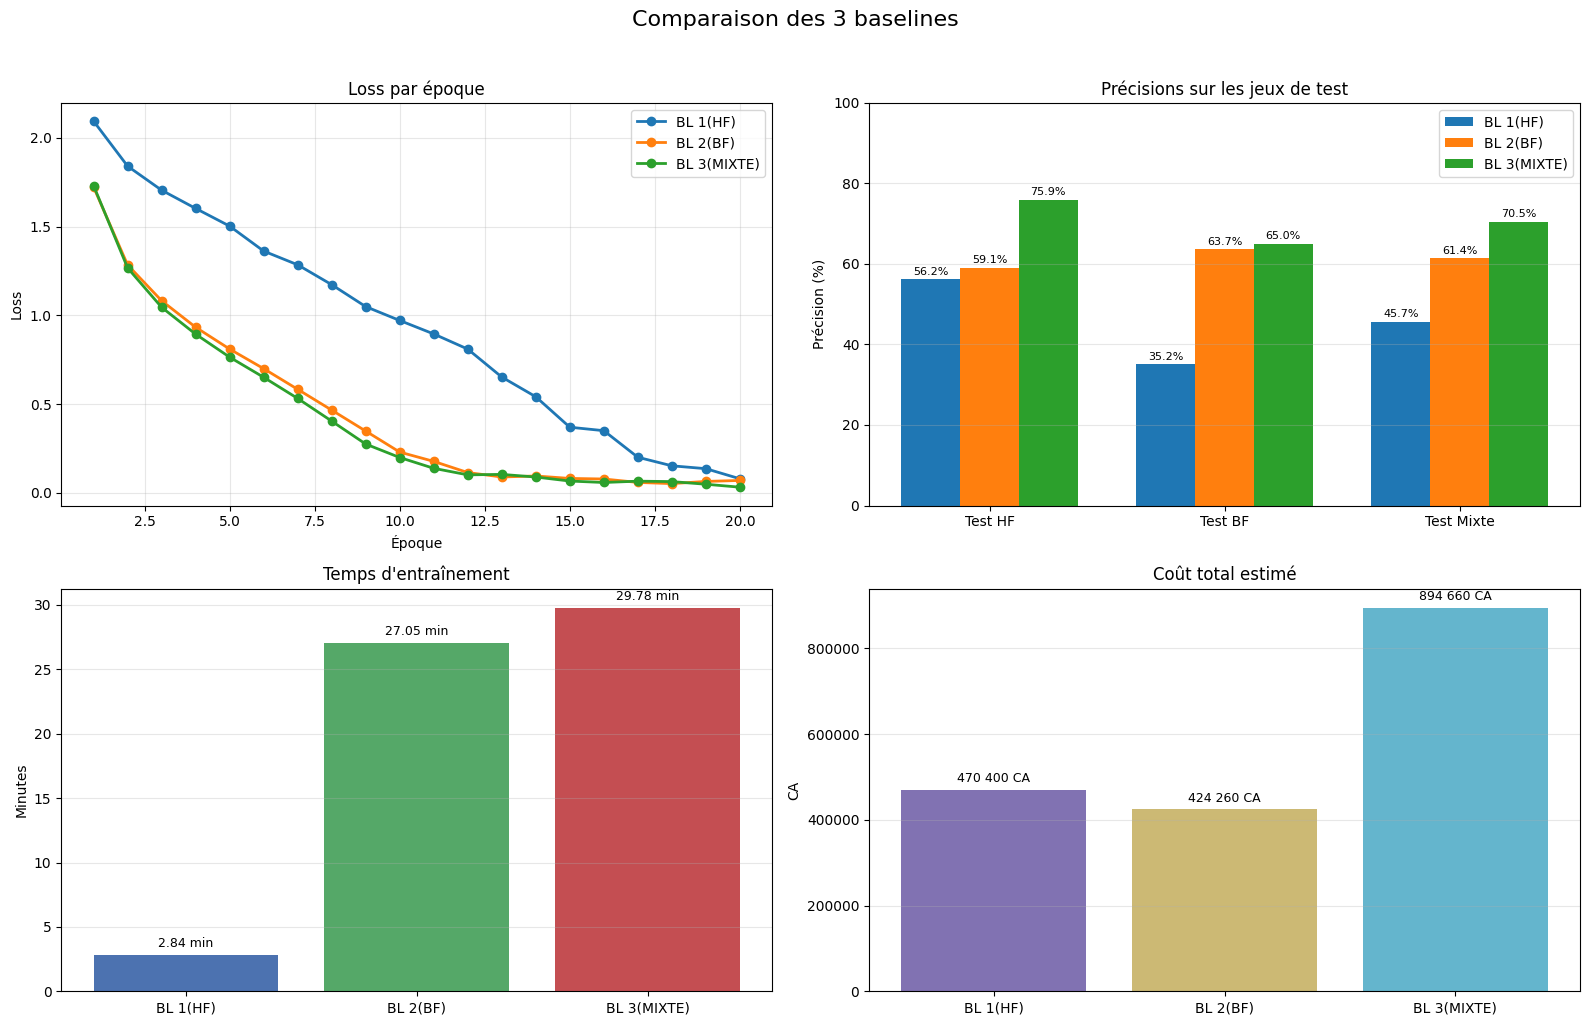
\includegraphics[width=\linewidth]{figures/baselines_comparison.png}
  \caption{Comparaison visuelle des trois baselines sur \textbf{Animals-10} (BL 1(HF), BL 2(BF), BL 3(MIXTE)) : loss par époque, précisions de test, temps d'entraînement et coût total estimé.}
  \label{fig:baseline_plots}
\end{figure}

\begin{hypothesebox}[Vérification sur Imagewoof]
  Réexécutées sur Imagewoof, les trois baselines confirment les conclusions tirées sur Animals-10, malgré des valeurs absolues nettement inférieures (Imagewoof = classification \textit{fine-grained} de races canines, $\approx$3$\times$ moins d'images d'entraînement) :
  \begin{itemize}
    \item \textbf{Domain Shift confirmé} : la BL 1 passe de 25,0\,\% (HF) à 22,1\,\% (BF) ; la chute est moins spectaculaire qu'ailleurs uniquement parce que la BL 1 est déjà très faible en HF sur ce problème difficile.
    \item \textbf{Paradoxe de la quantité confirmé} : la BL 2 (coût donnée 8 126 CA) bat la BL 1 (8 990 CA) sur les trois tests, y compris HF (42,7\,\% vs 25,0\,\%), avec un coût inférieur.
    \item \textbf{Borne supérieure validée} : la BL 3 atteint 50,3\,\% sur HF, meilleur score, pour un coût donnée double de BL 1.
  \end{itemize}
  La \textbf{hiérarchie BL 3 $>$ BL 2 $>$ BL 1} est strictement conservée, ce qui valide la robustesse des conclusions indépendamment du dataset.
\end{hypothesebox}

\begin{figure}[htbp]
  \centering
  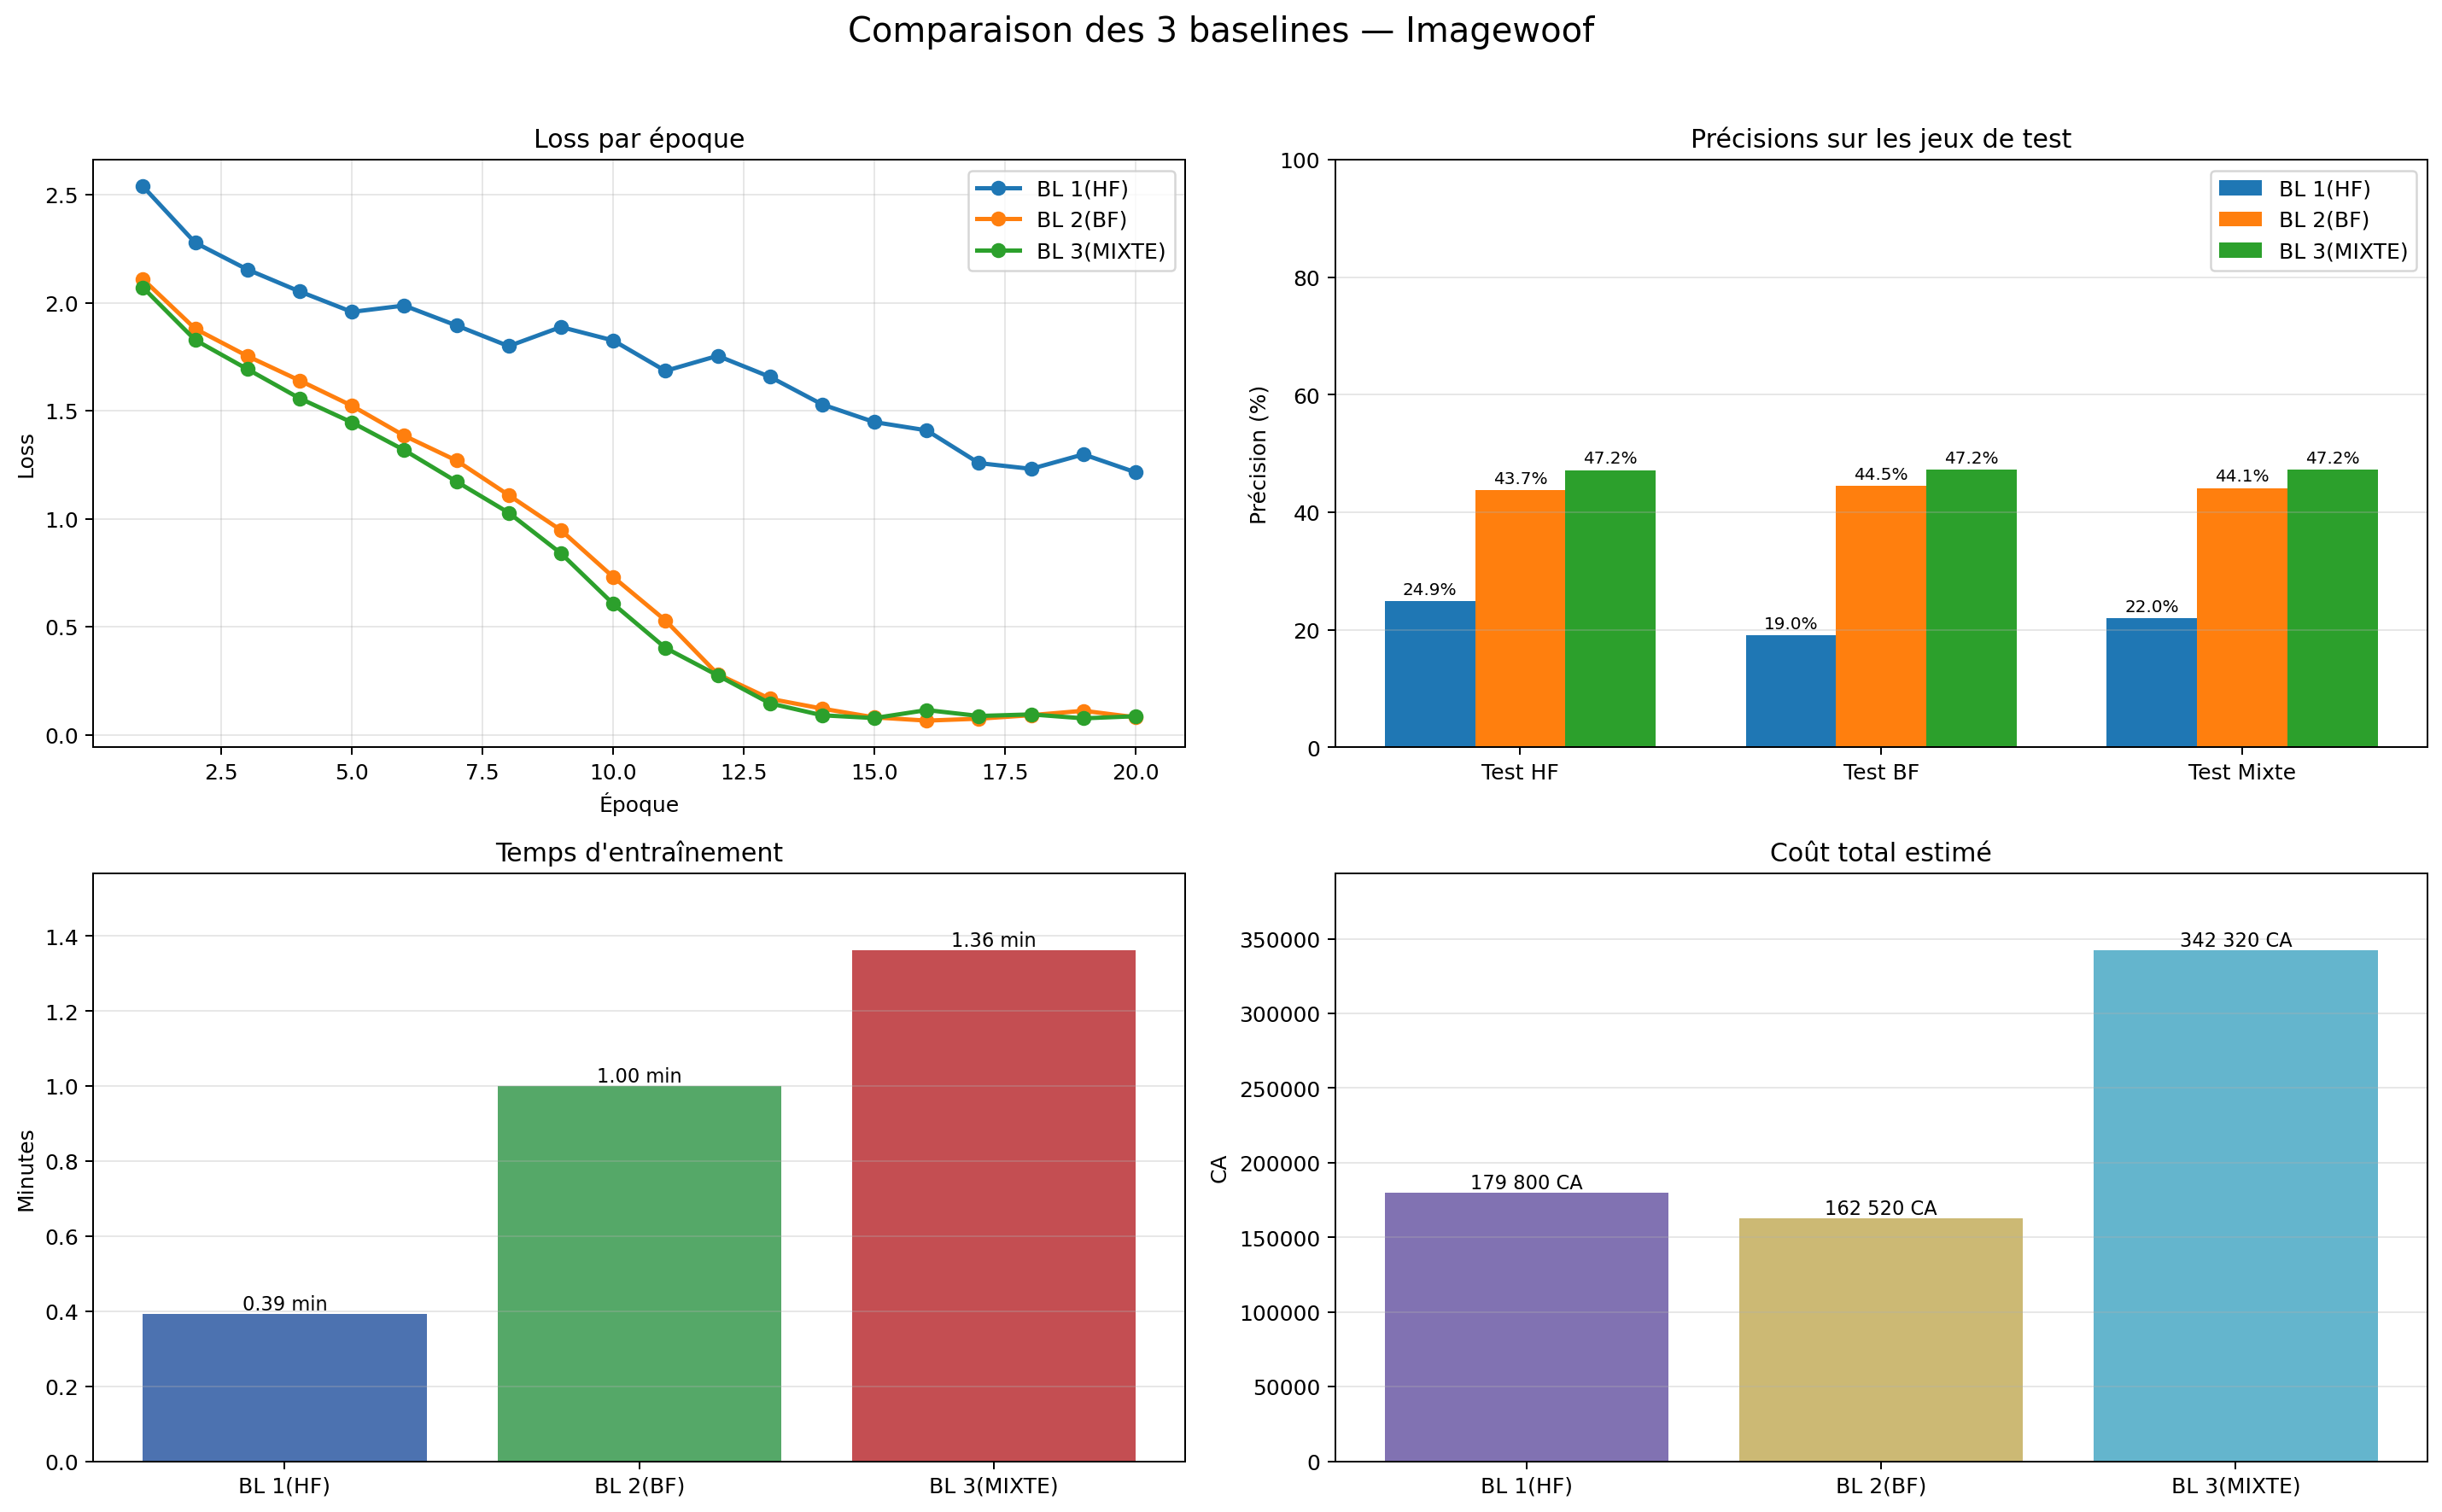
\includegraphics[width=\linewidth]{figures/baselines_comparison_imagewoof.png}
  \caption{Comparaison visuelle des trois baselines sur \textbf{Imagewoof} : précisions de test, temps d'entraînement et coût total estimé. Les valeurs absolues sont plus basses qu'Animals-10 (classification fine-grained) mais la hiérarchie BL 3 $>$ BL 2 $>$ BL 1 est strictement identique.}
  \label{fig:baseline_plots_imagewoof}
\end{figure}

\begin{hypothesebox}[Vérification sur Intel]
  Sur Intel (6 classes de scènes, tâche de nature différente), les valeurs absolues sont nettement plus hautes — la reconnaissance de scènes est plus facile que la classification fine-grained — mais la hiérarchie reste identique :
  \begin{itemize}
    \item \textbf{Domain Shift très marqué} : la BL 1 chute de 75,8\,\% (HF) à 47,0\,\% (BF), soit $-28,8$ points, l'effondrement le plus net des trois datasets.
    \item \textbf{Paradoxe de la quantité confirmé} : la BL 2 (coût donnée 12 632 CA) dépasse la BL 1 (14 020 CA) sur les trois tests, HF compris (78,7\,\% vs 75,8\,\%), et se montre remarquablement robuste sur BF (81,9\,\%).
    \item \textbf{Borne supérieure validée} : la BL 3 plafonne le panel (82,8\,\% HF, 82,5\,\% Mixte) pour le coût le plus élevé.
  \end{itemize}
  La \textbf{hiérarchie BL 3 $>$ BL 2 $>$ BL 1} se vérifie donc sur les \textbf{trois} datasets, malgré des volumes, granularités et natures de tâche très différents.
\end{hypothesebox}


% ============================================================
%  CHAPITRE 4
% ============================================================
\chapter{Stratégies Multi-Fidélité}

Ce chapitre présente les stratégies multi-fidélité, toutes orientées vers un \textbf{objectif HF prioritaire} : maximiser la performance sur données propres (Test HF) tout en exploitant le volume d'images BF bon marché pour réduire le coût. Quatre stratégies sont étudiées, chacune sur les trois datasets et en multi-seed (moyenne $\pm$ écart-type) :

\begin{itemize}
  \item \textbf{Stratégie 1 — Transfer Learning séquentiel} (BF~$\rightarrow$~HF) : pré-entraînement sur le volume BF puis fine-tuning sur le sous-ensemble HF ;
  \item \textbf{Stratégie 2 — Co-training pondéré} : les deux domaines sont vus simultanément dans chaque lot, avec une pondération explicite de la perte ;
  \item \textbf{Stratégie 3 — Curriculum Learning progressif} : la proportion d'images HF augmente par paliers au fil des époques (du tout-BF vers le tout-HF) ;
  \item \textbf{Stratégie 4 — Elastic Weight Consolidation (EWC)} : variante du transfert séquentiel où une pénalité de Fisher protège, pendant le fine-tuning HF, les poids importants pour le domaine BF (lutte contre l'oubli catastrophique).
\end{itemize}

Chaque stratégie est en outre déclinée en une version dont les hyperparamètres ont été optimisés par \textbf{Optuna} ; l'analyse détaillée de ces gains fait l'objet d'un chapitre dédié, les sections ci-dessous portant sur les configurations de base.

\section{Stratégie 1 -- Transfer Learning Séquentiel (BF $\rightarrow$ HF)}

% ---- 4.1.1 Protocole ----
\subsection{Protocole}

La stratégie retenue repose sur deux phases d'entraînement consécutives avec la même architecture ResNet-18 :

\begin{enumerate}
  \item \textbf{Pré-entraînement BF} : apprentissage sur le volume principal de données dégradées pour acquérir une représentation robuste et générique des classes.
  \item \textbf{Fine-tuning HF} : spécialisation sur un sous-ensemble HF plus petit, afin de récupérer les détails discriminants de haute fidélité.
\end{enumerate}

Configuration expérimentale utilisée :

\vspace{0.6em}
\renewcommand{\arraystretch}{1.45}
\begin{tabularx}{\linewidth}{L{4.1cm} C{3cm} L{7.6cm}}
  \arrayrulecolor{midgray}
  \toprule
  \tableheadcolor
  \textbf{Paramètre} & \textbf{Valeur} & \textbf{Commentaire} \\
  \midrule
  Architecture & ResNet-18 & Entraînée \textit{from scratch}, tête de classification 10 classes \\
  Optimiseur & Adam & Identique aux baselines pour conserver la comparabilité \\
  Batch size & 64 & Compromis stabilité/vitesse sur GPU V100S \\
  Époques BF & 10 & 21\,213 images BF (332 batches/époque) \\
  Époques HF & 10 & 1\,881 images HF train + 471 images HF val \\
  Learning rates & 0,001 puis 0,0003 & Plus faible en fine-tuning pour stabiliser l'adaptation \\
  Accélération & AMP (FP16) & \texttt{autocast} + \texttt{GradScaler} \\
  \bottomrule
\end{tabularx}

% ---- 4.1.2 Résultats ----
\subsection{Résultats quantitatifs obtenus}

Les résultats finaux de la Stratégie 1 sont résumés ci-dessous pour les trois datasets (moyenne $\pm$ écart-type sur 3 graines).
Dans cette étude, le critère prioritaire est la performance sur \textbf{Test HF}.

\vspace{0.6em}
\setlength{\tabcolsep}{4pt}
\renewcommand{\arraystretch}{1.45}
\begin{tabularx}{\linewidth}{L{2.6cm} C{2.45cm} C{2.45cm} C{2.45cm} C{2cm} C{2cm}}
  \arrayrulecolor{midgray}
  \toprule
  \tableheadcolor
  \textbf{Dataset} & \textbf{Test HF} & \textbf{Test BF} & \textbf{Test Mixte} & \textbf{Coût donnée} & \textbf{Coût total} \\
  \midrule
  \tablerowodd
  Animals-10 & \res{77,7}{0,6} & \res{68,3}{0,5} & \res{73,0}{0,3} & 44 733 & 400 230 \\
  Imagewoof  & \res{51,0}{1,6} & \res{44,7}{1,3} & \res{47,9}{1,5} & 17 116 & 153 160 \\
  \tablerowodd
  Intel      & \res{86,1}{0,4} & \res{79,1}{1,4} & \res{82,6}{0,7} & 26 652 & 238 420 \\
  \bottomrule
\end{tabularx}
\setlength{\tabcolsep}{6pt}

\vspace{0.8em}
\begin{hypothesebox}[Lecture rapide des courbes d'entraînement (Animals-10, graine 42)]
  La phase BF converge rapidement en \textit{train loss}, alors que la validation HF fluctue fortement pendant le pré-entraînement.
  Après transition vers HF, la précision validation HF bondit immédiatement autour de 77--78\,\%, puis se stabilise ; la \textit{val loss} remonte légèrement en fin de fine-tuning, signalant un début de sur-apprentissage. Sur les 3 graines, le score final HF est très stable (77,7~$\pm$~0,6\,\%).
\end{hypothesebox}

\begin{figure}[htbp]
  \centering
  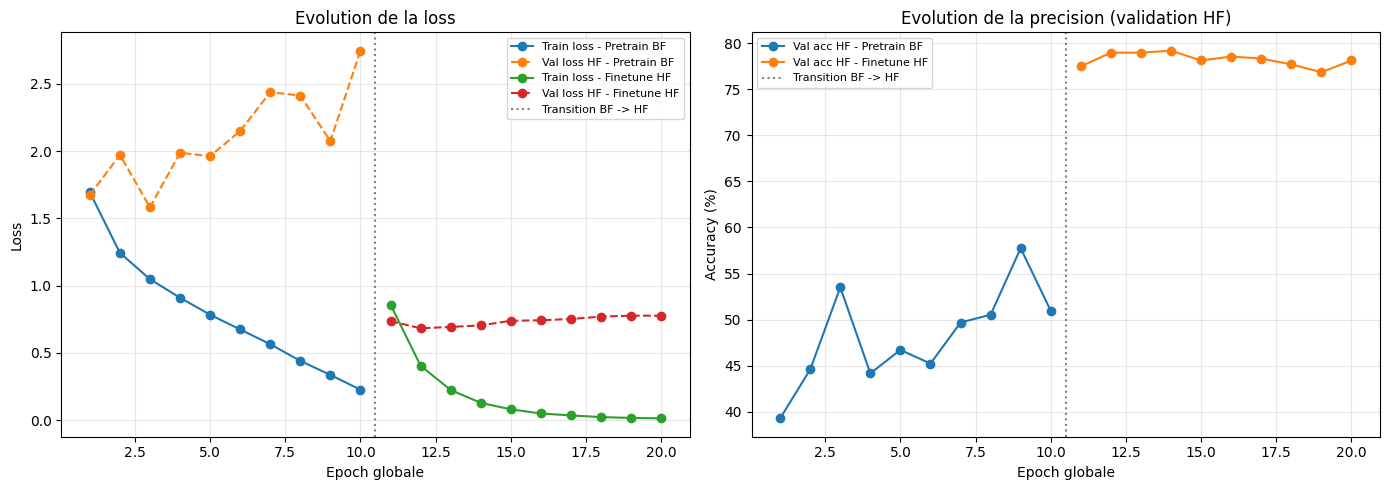
\includegraphics[width=\linewidth]{figures/strategy1_transfer_learning_curves.png}
  \caption{Évolution de la loss et de la précision validation HF pendant le pré-entraînement BF puis le fine-tuning HF, sur \textbf{Animals-10}.}
  \label{fig:strategy1_curves_placeholder}
\end{figure}

\begin{figure}[htbp]
  \centering
  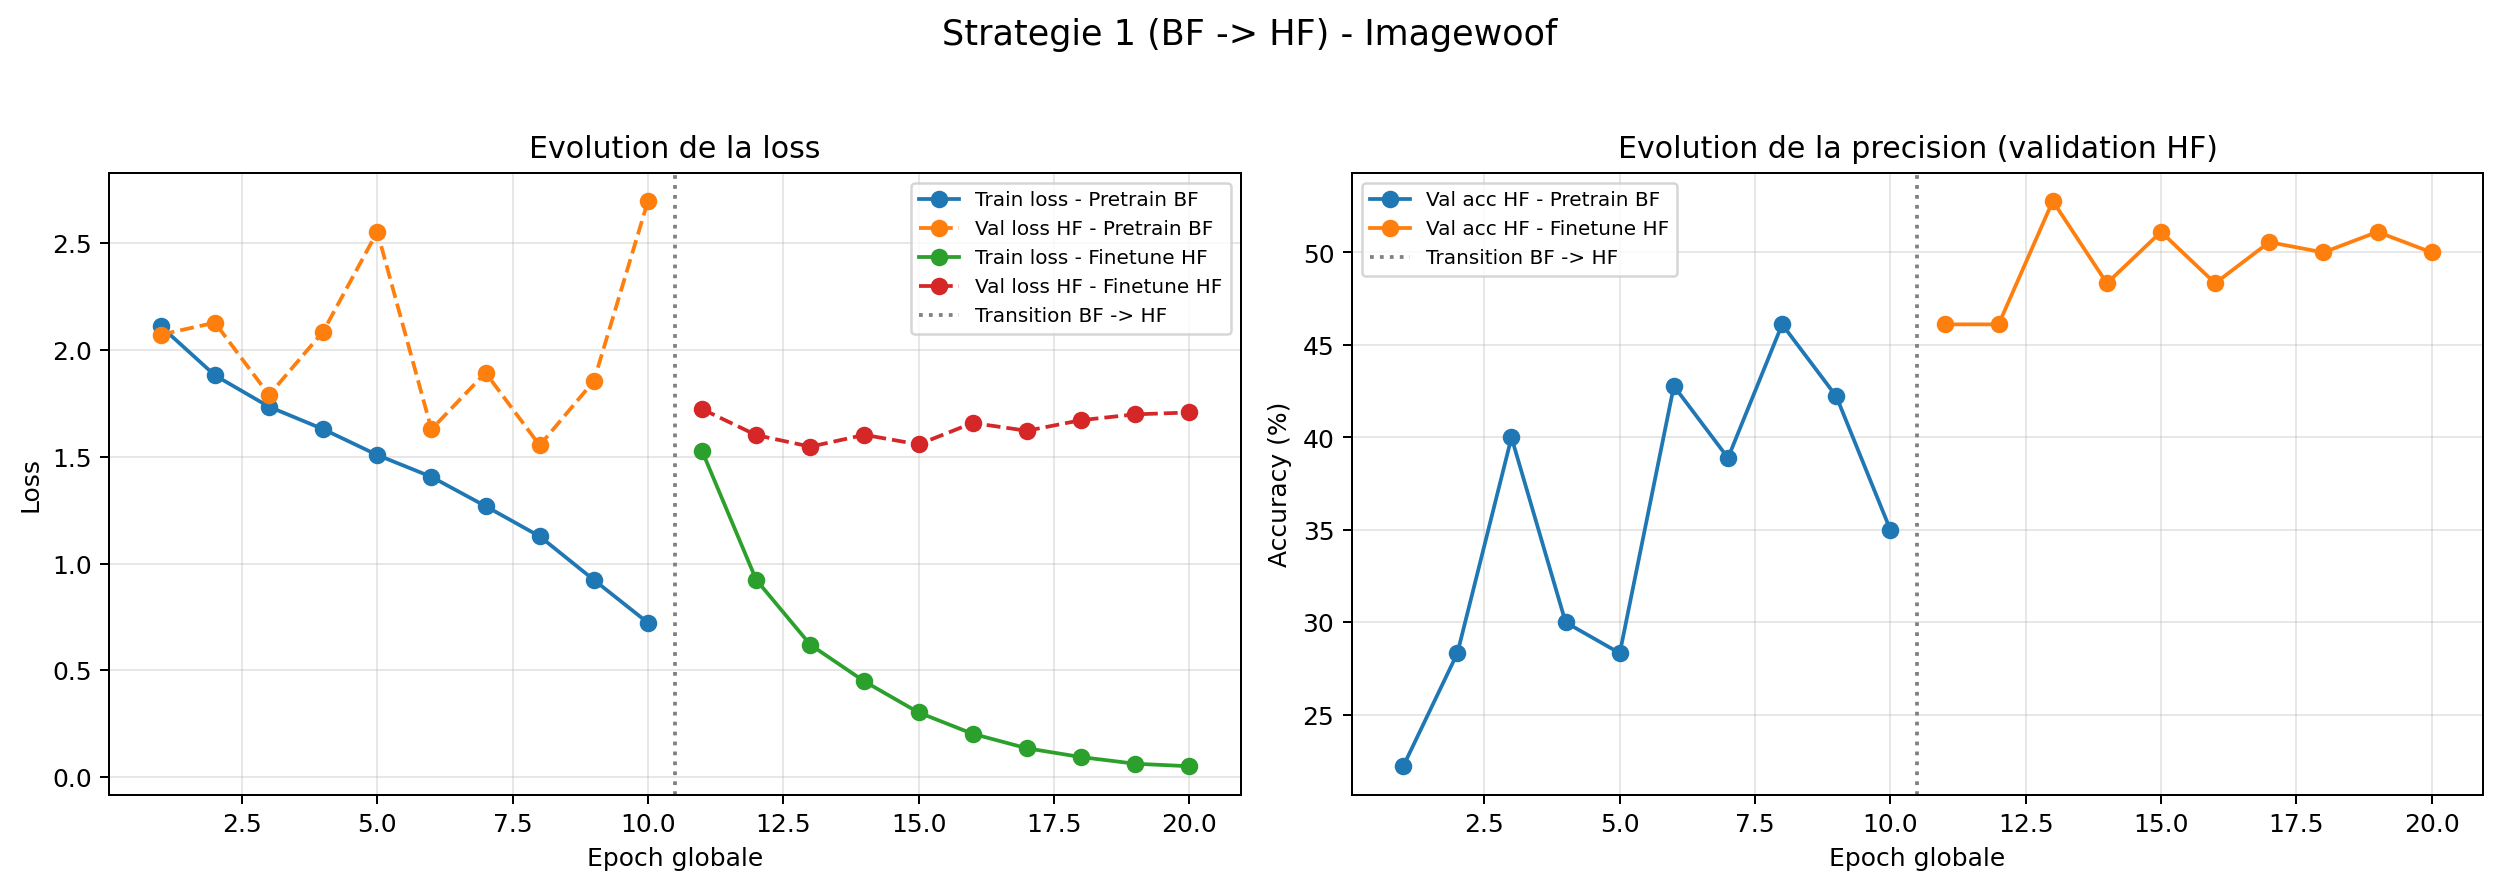
\includegraphics[width=\linewidth]{figures/strategy1_transfer_learning_curves_imagewoof.png}
  \caption{Évolution de la loss et de la précision validation HF pendant le pré-entraînement BF puis le fine-tuning HF, sur \textbf{Imagewoof}.}
  \label{fig:strategy1_curves_imagewoof}
\end{figure}

% ---- 4.1.3 Comparaison ----
\subsection{Comparaison avec les baselines}

Les valeurs chiffrées détaillées figurent dans le \textbf{tableau de synthèse global} (§4.4.3), qui rassemble toutes les approches sur les trois datasets. La comparaison se concentre ici sur l'écart à la borne supérieure, la \textbf{baseline Mixte (BL 3)}.

\vspace{0.4em}
Comparaisons clés (Animals-10) :

\begin{itemize}
  \item \textbf{Objectif principal HF atteint} : la Stratégie 1 obtient \textbf{77,7\,\% sur Test HF}, supérieure à \textbf{toutes les baselines} (BL 3 = 74,0\,\%, BL 2 = 61,3\,\%, BL 1 = 54,3\,\%), et avec le plus faible écart-type (0,6), donc la plus stable.
  \item \textbf{Vs BL 3 (Mixte)} : à \textbf{coût donnée identique} (44 733 CA, même pool HF+BF), elle dépasse BL 3 sur HF ($+3,7$ points) tout en réduisant le \textbf{coût total} de $\approx$\,55\,\% (894 660 $\rightarrow$ 400 230 CA), car le HF coûteux n'est vu qu'en phase de fine-tuning.
  \item \textbf{Compromis BF modéré} : la précision BF (68,3\,\%) reste légèrement inférieure à BL 2 (71,0\,\%) et BL 3 (72,9\,\%), compromis cohérent avec la priorité explicitement fixée sur la qualité HF.
\end{itemize}

\begin{hypothesebox}[Vérification sur Imagewoof et Intel]
  La Stratégie 1 confirme son rang sur les deux datasets de validation, dépassant les trois baselines sur Test HF :
  \begin{itemize}
    \item \textbf{Imagewoof} : 51,0\,\% HF, soit le meilleur score parmi baselines et S1 (BL 3 = 50,3\,\%). L'avantage HF sur BL~3 est ténu ($+0,7$ point) mais le \textbf{coût total est divisé par $\approx$2,2} (153 160 vs 342 320 CA) à coût donnée identique — l'intérêt de la séparation BF~$\rightarrow$~HF est ici surtout économique.
    \item \textbf{Intel} : 86,1\,\% HF, nettement devant BL 3 (82,8\,\%), $+3,3$ points, là encore pour un coût total réduit de plus de moitié (238 420 vs 533 040 CA).
  \end{itemize}
  La hiérarchie \textbf{Stratégie 1 $>$ BL 3 $>$ BL 2 $>$ BL 1} sur Test HF est \textbf{strictement identique sur les trois datasets}, ce qui confirme que la dominance du transfer learning séquentiel sur les baselines n'est pas un artefact d'un jeu de données particulier.
\end{hypothesebox}

% ---- 4.1.4 Analyse ----
\subsection{Analyse : ce qui a marché, ce qui a moins marché, et enseignements}

\begin{itemize}
  \item \textbf{Ce qui a bien marché (HF)} : la phase BF fournit une initialisation robuste, puis le fine-tuning HF spécialise efficacement le modèle ; le gain final en Test HF est net et place la Stratégie 1 en tête.
  \item \textbf{Limite observée} : la spécialisation HF entraîne une perte partielle de robustesse BF (\textit{domain forgetting}), ce qui était attendu dans une optimisation orientée domaine propre.
  \item \textbf{Signal de sur-apprentissage léger} : en fin de fine-tuning, la \textit{train loss} continue de baisser tandis que la \textit{val loss} HF se dégrade légèrement ; un \textit{early stopping} piloté par Test/Val HF améliorerait encore la stabilité.
  \item \textbf{Leçon principale} : pour un objectif centré sur la performance HF, le transfer learning séquentiel offre le meilleur compromis observé entre précision cible et coût d'annotation.
\end{itemize}

\begin{decisionbox}
  \textbf{Conclusion (Stratégie 1, objectif HF prioritaire) :} la stratégie BF $\rightarrow$ HF est validée comme meilleure option actuelle pour maximiser la performance sur données propres. La Stratégie 2 (co-training pondéré) visera désormais à conserver ce niveau HF tout en regagnant de la robustesse sur BF.
\end{decisionbox}

\section{Stratégie 2 -- Co-training par Batch avec Pondération (Reweighting)}

% ---- 4.2.1 Protocole ----
\subsection{Protocole}

Contrairement à la stratégie séquentielle BF $\rightarrow$ HF, cette approche entraîne le modèle sur les deux domaines \textbf{au sein d'un même lot}. L'idée est de conserver la diversité BF tout en imposant une priorité d'optimisation sur les exemples HF, considérés comme plus fiables.

Deux mécanismes sont appliqués conjointement :

\begin{enumerate}
  \item \textbf{Co-training à ratio fixe par batch} : chaque lot contient exactement 16 images HF et 48 images BF (batch size = 64), soit un ratio HF de 25\%.
  \item \textbf{Loss pondérée par domaine}~\cite{ren2018reweight,han2018coteaching} : la perte individuelle est multipliée par un poids plus fort sur HF ($w_{HF}=2.0$) et plus faible sur BF ($w_{BF}=0.7$), avant agrégation.
\end{enumerate}

Configuration expérimentale utilisée :

\vspace{0.6em}
\renewcommand{\arraystretch}{1.45}
\begin{tabularx}{\linewidth}{L{4.1cm} C{3cm} L{7.6cm}}
  \arrayrulecolor{midgray}
  \toprule
  \tableheadcolor
  \textbf{Paramètre} & \textbf{Valeur} & \textbf{Commentaire} \\
  \midrule
  Architecture & ResNet-18 & Entraînée \textit{from scratch}, classifieur 10 classes \\
  Optimiseur & Adam & Même famille d'optimisation que les expériences précédentes \\
  Batch size & 64 & Composition contrôlée HF/BF à chaque itération \\
  Époques & 20 & Entraînement conjoint sur 117 batches par époque \\
  Ratio batch & 16 HF / 48 BF & Ratio HF fixé à 25\% par \textit{MixedBatchSampler} \\
  Poids de loss & HF: 2.0 ; BF: 0.7 & Accent mis sur les erreurs HF dans la mise à jour des gradients \\
  Données utilisées & 1\,881 HF train + 21\,213 BF train & Validation sur 471 HF ; test sur 2\,614 images \\
  \bottomrule
\end{tabularx}

% ---- 4.2.2 Résultats ----
\subsection{Résultats quantitatifs obtenus}

Les résultats finaux de la Stratégie 2 sont résumés ci-dessous pour les trois datasets (moyenne $\pm$ écart-type sur 3 graines).
Le critère prioritaire reste la précision sur \textbf{Test HF}.

\vspace{0.6em}
\setlength{\tabcolsep}{4pt}
\renewcommand{\arraystretch}{1.45}
\begin{tabularx}{\linewidth}{L{2.6cm} C{2.45cm} C{2.45cm} C{2.45cm} C{2cm} C{2cm}}
  \arrayrulecolor{midgray}
  \toprule
  \tableheadcolor
  \textbf{Dataset} & \textbf{Test HF} & \textbf{Test BF} & \textbf{Test Mixte} & \textbf{Coût donnée} & \textbf{Coût total} \\
  \midrule
  \tablerowodd
  Animals-10 & \res{63,8}{5,2} & \res{61,0}{4,2} & \res{62,4}{4,7} & 44 733 & 486 720 \\
  Imagewoof  & \res{37,5}{0,8} & \res{37,4}{0,3} & \res{37,5}{0,2} & 17 116 & 183 040 \\
  \tablerowodd
  Intel      & \res{82,0}{1,0} & \res{79,8}{0,9} & \res{80,9}{0,9} & 26 652 & 291 200 \\
  \bottomrule
\end{tabularx}
\setlength{\tabcolsep}{6pt}

\vspace{0.8em}
\begin{hypothesebox}[Lecture rapide des courbes d'entraînement (Animals-10, graine 42)]
  La \textit{train weighted loss} décroît régulièrement, avec une baisse plus rapide de la loss HF non pondérée que de la loss BF, ce qui confirme l'effet attendu du \textit{reweighting}.
  La validation HF progresse globalement mais avec des oscillations intermédiaires marquées, signe d'une optimisation \textbf{plus instable} qu'en stratégie séquentielle — instabilité que confirme le fort écart-type inter-graines du score final (63,8~$\pm$~5,2\,\%).
\end{hypothesebox}

\begin{figure}[htbp]
  \centering
  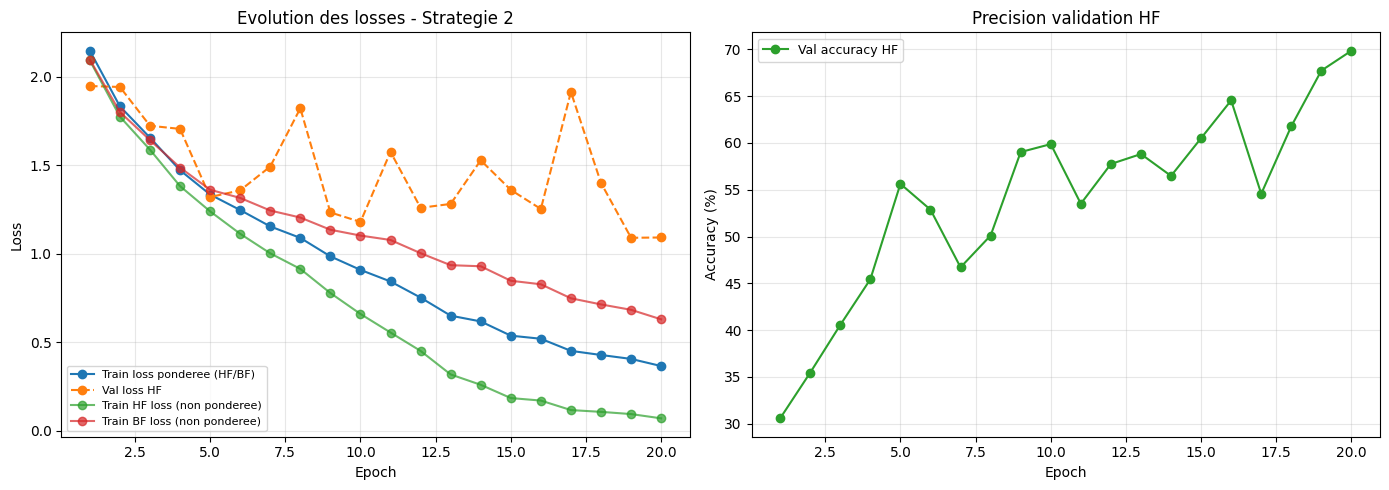
\includegraphics[width=\linewidth]{figures/strategy2_cotraining_reweighting_curves.png}
  \caption{Évolution des losses et de la précision validation HF pour la Stratégie 2 (co-training pondéré HF/BF) sur \textbf{Animals-10}.}
  \label{fig:strategy2_cotraining_curves}
\end{figure}

\begin{figure}[htbp]
  \centering
  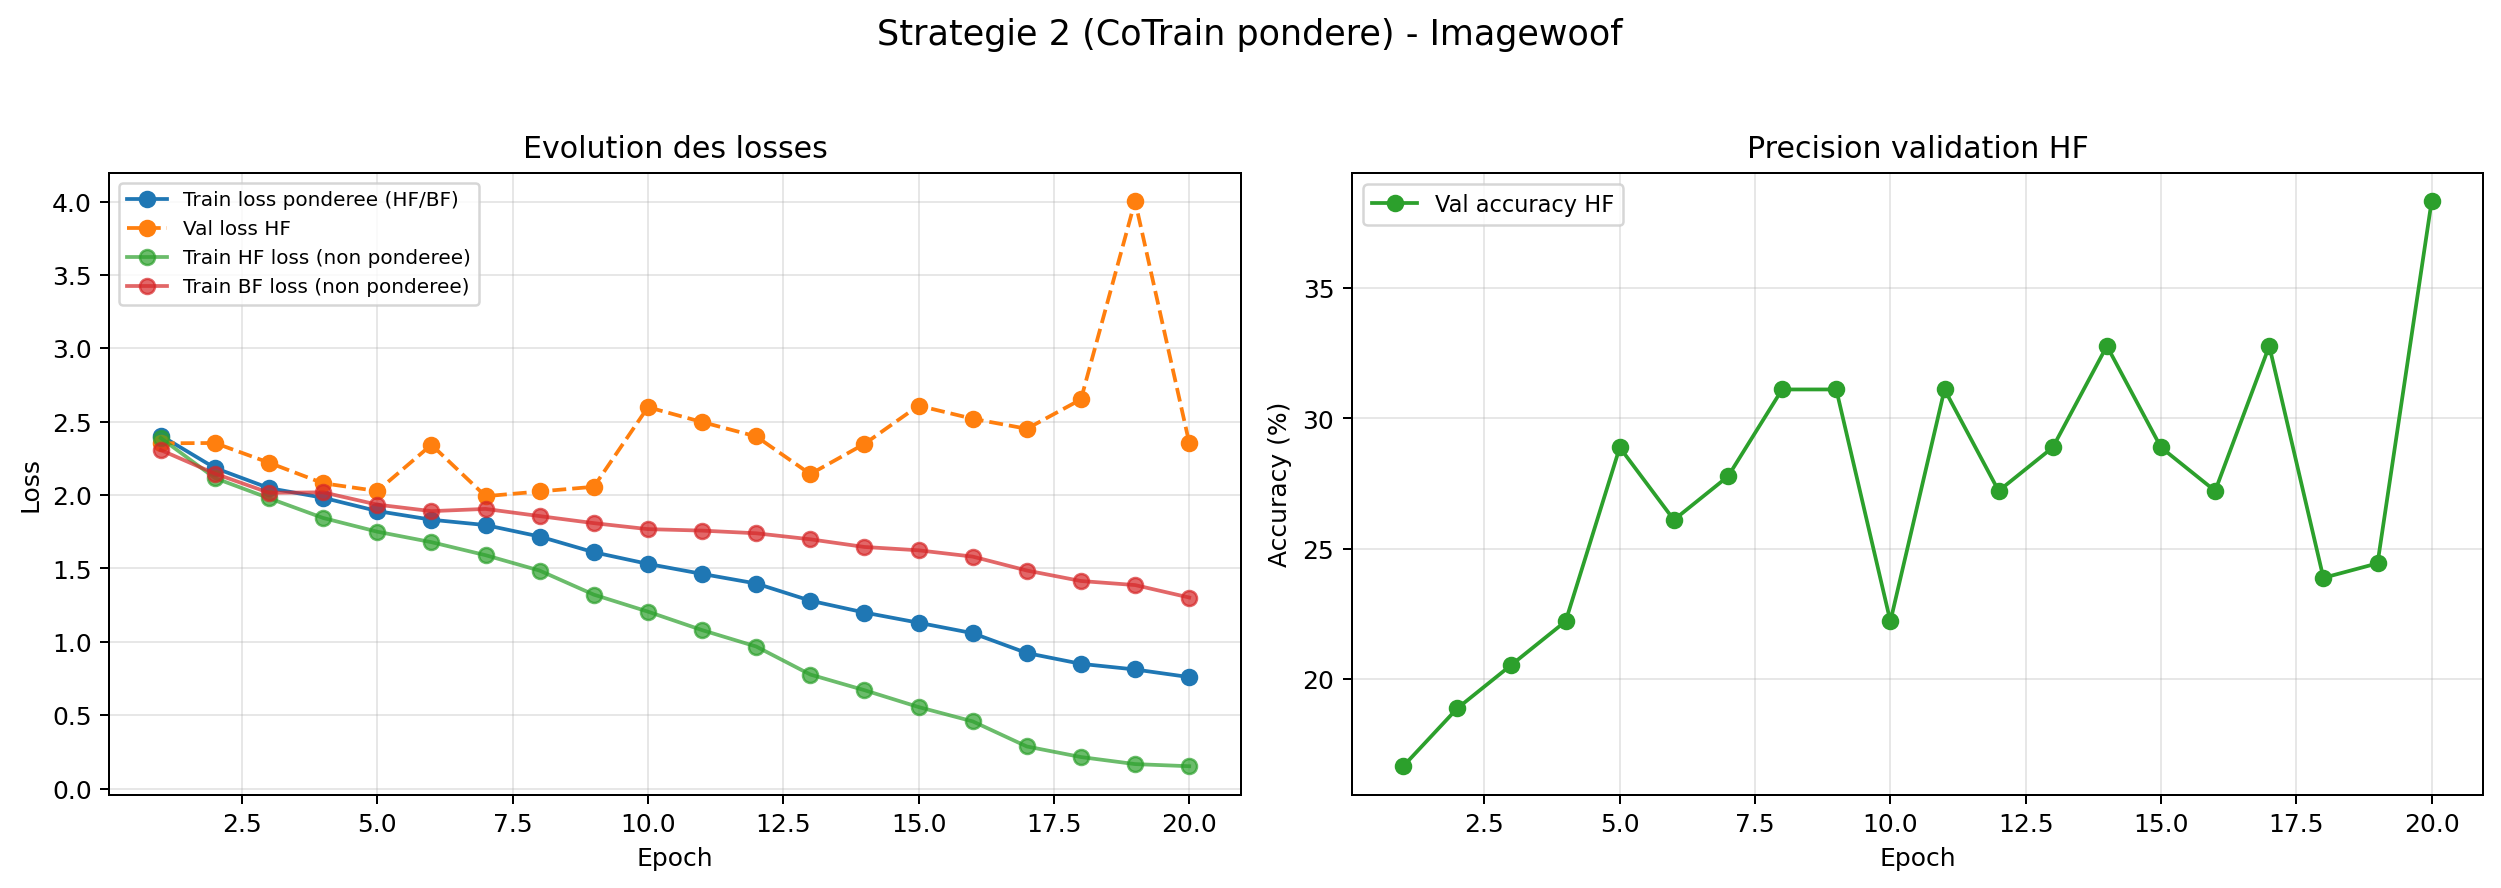
\includegraphics[width=\linewidth]{figures/strategy2_cotraining_reweighting_curves_imagewoof.png}
  \caption{Évolution des losses et de la précision validation HF pour la Stratégie 2 sur \textbf{Imagewoof}.}
  \label{fig:strategy2_cotraining_curves_imagewoof}
\end{figure}

% ---- 4.2.3 Comparaison ----
\subsection{Comparaison avec les baselines et la Stratégie 1}

Les valeurs chiffrées détaillées figurent dans le \textbf{tableau de synthèse global} (§4.4.3). La comparaison ci-dessous situe la Stratégie 2 par rapport à la \textbf{baseline Mixte (BL 3)} et à la \textbf{Stratégie 1}.

\vspace{0.4em}
Comparaisons clés (Animals-10) :

\begin{itemize}
  \item \textbf{Gain HF modéré vs baselines} : la Stratégie 2 atteint 63,8\,\% sur Test HF, devant BL 1 (54,3\,\%) et BL 2 (61,3\,\%), mais l'avantage sur BL 2 est faible ($+2,5$ points).
  \item \textbf{Dominée par la Stratégie 1} : contre-intuitivement, la Stratégie 2 est ici inférieure à la stratégie séquentielle \textbf{à la fois sur HF} ($-13,9$ points : 63,8\,\% vs 77,7\,\%) \textbf{et sur BF} ($-7,3$ points : 61,0\,\% vs 68,3\,\%). Voir les deux domaines en même temps ne suffit pas à égaler une spécialisation HF finale explicite.
  \item \textbf{Instabilité marquée} : avec des écarts-types de 4 à 5 points, le co-training pondéré est nettement \textbf{moins stable} que les autres stratégies (S1 $<$~1 point), ce qui complique la sélection de modèle.
  \item \textbf{Coût intermédiaire} : son coût total (486 720 CA) est inférieur à BL 3 (894 660 CA) mais supérieur à la Stratégie 1 (400 230 CA), pour une performance moindre.
\end{itemize}

\begin{hypothesebox}[Vérification sur Imagewoof et Intel]
  La Stratégie 2 se révèle \textbf{très sensible au volume HF et au type de tâche} :
  \begin{itemize}
    \item \textbf{Imagewoof (décrochage)} : 37,5\,\% HF seulement, sous BL 2 (42,7\,\%), BL 3 (50,3\,\%) et loin de la Stratégie 1 (51,0\,\%) ; seule BL 1 fait pire. Le faible volume HF ($\approx$720 images train) ne permet pas au \textit{reweighting} de spécialiser les \textit{features} fine-grained, le batch étant mécaniquement dominé par les 48 échantillons BF sur 64. Son seul atout reste un équilibre HF/BF extrêmement resserré (37,5\,/\,37,4).
    \item \textbf{Intel (correcte mais jamais en tête)} : 82,0\,\% HF, au-dessus des baselines mono-domaine (BL 1, BL 2) mais en dessous de BL 3 (82,8\,\%) et surtout de la Stratégie 1 (86,1\,\%).
  \end{itemize}
  Bilan : sur les trois datasets, la Stratégie 2 n'est \textbf{jamais la meilleure} et souffre d'une forte variance ou d'un décrochage selon le dataset. Son intérêt conceptuel (équilibrage HF/BF) ne se traduit pas en performance HF maximale.
\end{hypothesebox}

% ---- 4.2.4 Analyse ----
\subsection{Analyse : ce qui a marché, ce qui a moins marché, et enseignements}

\begin{itemize}
  \item \textbf{Équilibrage HF/BF réel} : le mélange systématique HF/BF dans chaque batch produit l'écart HF$-$BF le plus resserré du panel (notamment sur Imagewoof), conforme à l'esprit de la méthode.
  \item \textbf{Effet du reweighting confirmé} : la décroissance plus rapide de la loss HF non pondérée montre que le modèle a effectivement priorisé les erreurs HF pendant l'optimisation.
  \item \textbf{Limite principale (objectif HF prioritaire)} : la Stratégie 2 ne retrouve pas le niveau HF de la Stratégie 1 — elle est même \textbf{dominée par S1 sur HF \emph{et} BF} sur Animals-10 — ce qui confirme qu'une spécialisation finale explicite sur HF reste plus efficace pour viser la performance maximale sur domaine propre.
  \item \textbf{Instabilité et sensibilité au dataset} : forte variance inter-graines (jusqu'à $\pm$5 points) et décrochage sur Imagewoof (faible volume HF) ; la méthode est peu robuste sans réglage fin du ratio et des poids.
\end{itemize}

\begin{decisionbox}
  \textbf{Conclusion (Stratégie 2, objectif HF prioritaire) :} le co-training pondéré tient sa promesse d'équilibrage HF/BF, mais il est \textbf{dominé par la Stratégie 1} sur la métrique cible (Test HF) et souffre d'instabilité. Les stratégies suivantes (Curriculum, EWC) chercheront à retrouver — voire dépasser — le niveau HF de la Stratégie 1 tout en améliorant la rétention BF et la stabilité.
\end{decisionbox}

\section{Stratégie 3 -- Curriculum Learning progressif}

% ---- 4.3.1 Protocole ----
\subsection{Protocole}

Le \textit{curriculum learning}~\cite{bengio2009curriculum} consiste à présenter les exemples du plus simple au plus complexe, à l'image d'un apprentissage humain. Nous l'adaptons au cadre multi-fidélité en faisant croître \textbf{progressivement la proportion d'images HF} au fil d'un \textbf{entraînement unique et continu} : le réseau démarre sur le volume BF abondant et bon marché (structures grossières, faciles), puis la part de HF augmente par paliers jusqu'à un fine-tuning final entièrement HF. Contrairement à la Stratégie 1, il n'y a pas de rupture nette BF~$\rightarrow$~HF mais une transition douce, ce qui vise à limiter l'oubli du domaine BF.

Le planning utilisé découpe les 20 époques en \textbf{quatre paliers} de 5 époques, à proportion d'images HF croissante :

\vspace{0.6em}
\renewcommand{\arraystretch}{1.45}
\begin{tabularx}{\linewidth}{C{3cm} C{2.6cm} L{8.4cm}}
  \arrayrulecolor{midgray}
  \toprule
  \tableheadcolor
  \textbf{Palier} & \textbf{Proportion HF} & \textbf{Rôle} \\
  \midrule
  \tablerowodd
  Époques 1--5   & 0 \%   & Tout-BF : apprentissage des structures grossières sur le volume abondant \\
  Époques 6--10  & 25 \%  & Introduction mesurée d'images nettes \\
  \tablerowodd
  Époques 11--15 & 60 \%  & Bascule majoritaire vers la haute fidélité \\
  Époques 16--20 & 100 \% & Fine-tuning final entièrement HF \\
  \bottomrule
\end{tabularx}

\vspace{0.6em}
Configuration : ResNet-18 \textit{from scratch}, optimiseur Adam, \textit{learning rate} $0{,}001$, batch size $64$, 20 époques, AMP (FP16) ; identique aux autres stratégies pour conserver la comparabilité.

% ---- 4.3.2 Résultats ----
\subsection{Résultats quantitatifs obtenus}

Résultats sur les trois datasets (moyenne $\pm$ écart-type sur 3 graines) ; critère prioritaire : \textbf{Test HF}.

\vspace{0.6em}
\setlength{\tabcolsep}{4pt}
\renewcommand{\arraystretch}{1.45}
\begin{tabularx}{\linewidth}{L{2.6cm} C{2.45cm} C{2.45cm} C{2.45cm} C{2cm} C{2cm}}
  \arrayrulecolor{midgray}
  \toprule
  \tableheadcolor
  \textbf{Dataset} & \textbf{Test HF} & \textbf{Test BF} & \textbf{Test Mixte} & \textbf{Coût donnée} & \textbf{Coût total} \\
  \midrule
  \tablerowodd
  Animals-10 & \res{76,5}{0,2} & \res{73,1}{0,1} & \res{74,8}{0,1} & 44 733 & 421 265 \\
  Imagewoof  & \res{47,5}{1,4} & \res{46,1}{1,1} & \res{46,8}{1,2} & 17 116 & 158 880 \\
  \tablerowodd
  Intel      & \res{84,6}{1,0} & \res{82,6}{1,5} & \res{83,6}{1,2} & 26 652 & 250 880 \\
  \bottomrule
\end{tabularx}
\setlength{\tabcolsep}{6pt}

\vspace{0.6em}
\begin{hypothesebox}[Signature de la méthode]
  Le curriculum progressif se distingue par deux traits remarquables : la \textbf{meilleure rétention BF de toutes les stratégies} (sur Animals-10, 73,1\,\% en BF, soit même \emph{au-dessus} de la baseline Mixte) et la \textbf{plus grande stabilité} inter-graines (écarts-types de l'ordre de 0,1--0,2 point sur Animals-10). La transition douce BF~$\rightarrow$~HF évite l'oubli brutal du domaine dégradé.
\end{hypothesebox}

\begin{figure}[htbp]
  \centering
  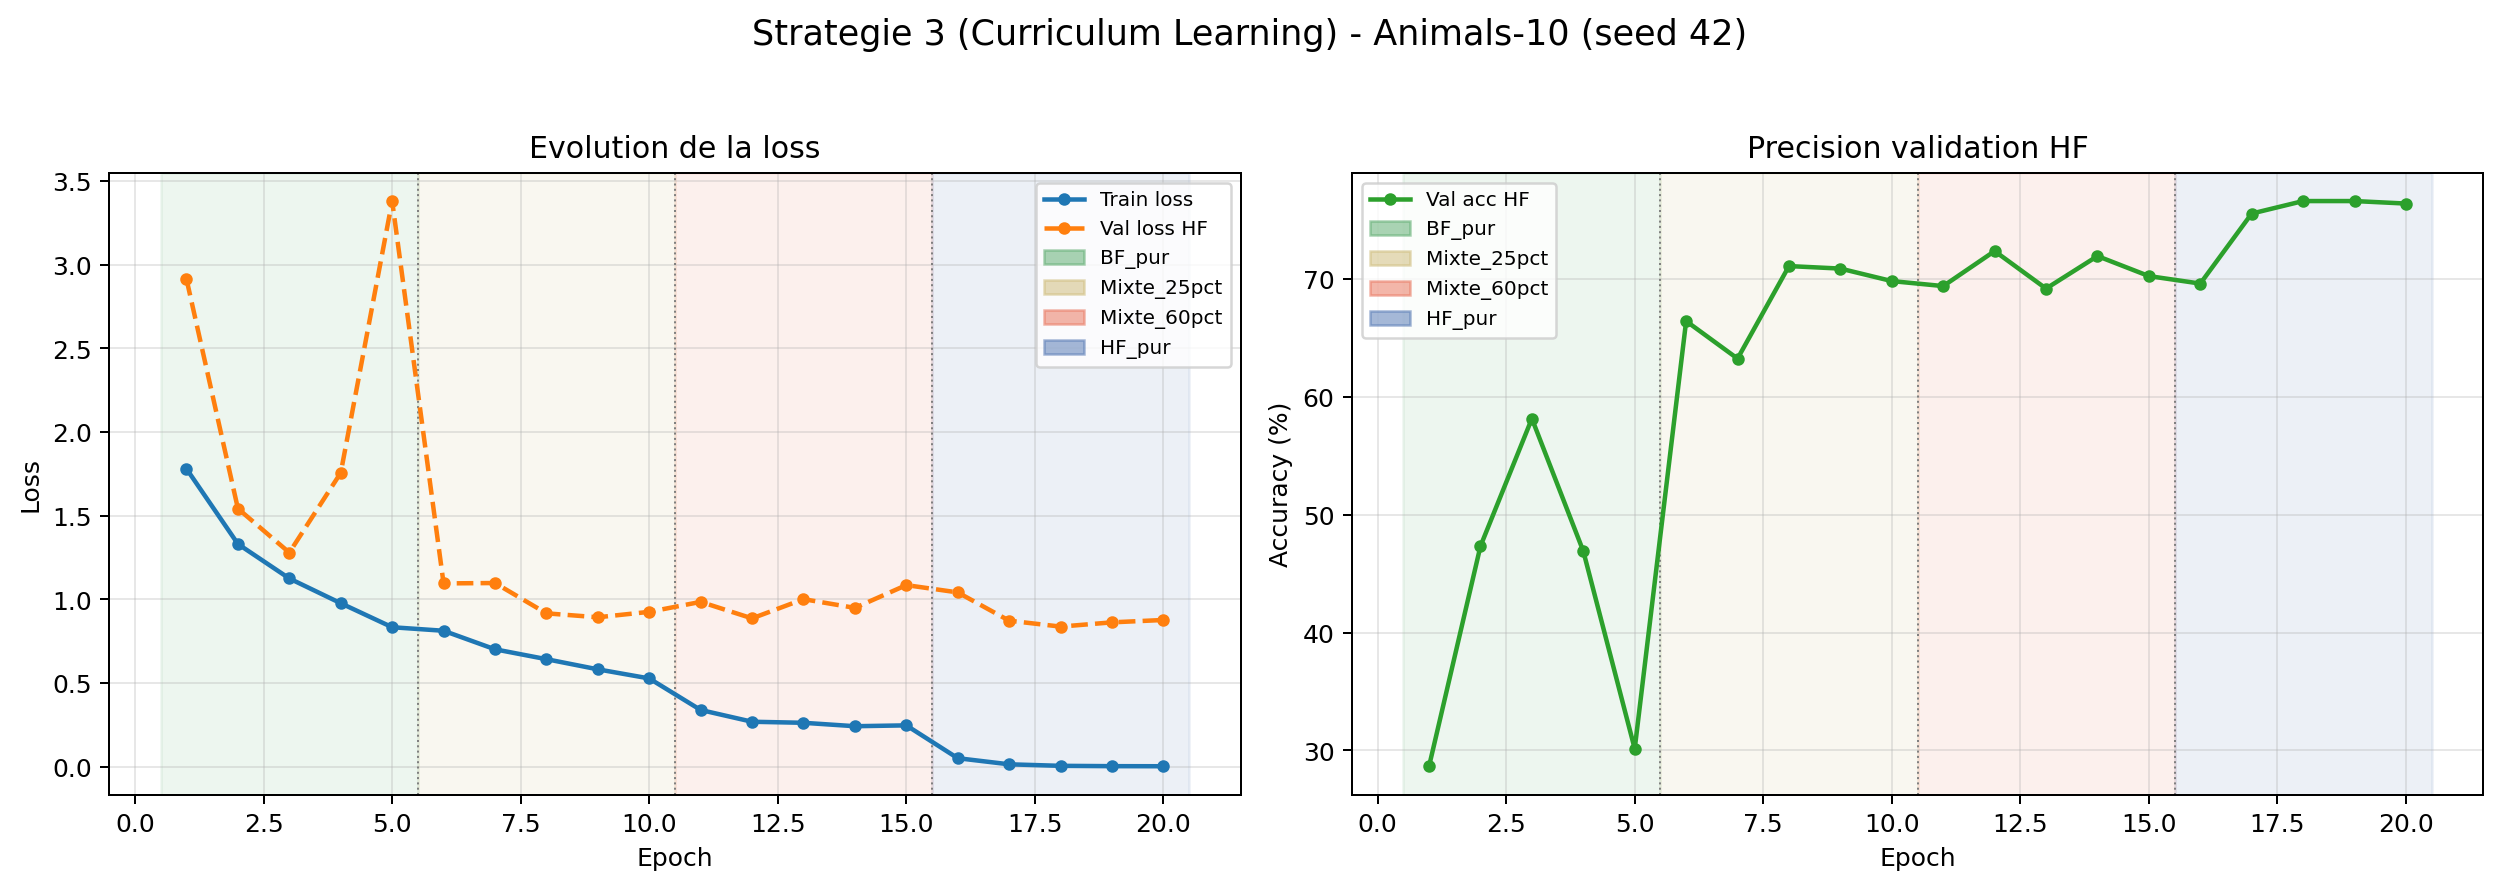
\includegraphics[width=\linewidth]{figures/strategy3_curriculum_curves.png}
  \caption{Évolution de la loss et de la précision validation HF pour la Stratégie 3 (curriculum progressif) sur \textbf{Animals-10}. La montée par paliers de la proportion HF (0~\% $\rightarrow$ 25~\% $\rightarrow$ 60~\% $\rightarrow$ 100~\%) se lit dans les inflexions de la courbe.}
  \label{fig:strategy3_curriculum_curves}
\end{figure}

% ---- 4.3.3 Comparaison ----
\subsection{Comparaison avec les baselines et les stratégies précédentes}

\begin{itemize}
  \item \textbf{Vs baseline Mixte (BL 3)} : à \textbf{coût donnée identique}, le curriculum dépasse BL 3 sur Test HF des trois datasets (Animals-10 : 76,5 vs 74,0 ; Intel : 84,6 vs 82,8 ; Imagewoof : 47,5 vs 50,3 — ici légèrement en deçà), tout en réduisant fortement le coût total (Animals-10 : 421 265 vs 894 660 CA, soit $-53$\,\%).
  \item \textbf{Vs Stratégie 1 (séquentielle)} : le curriculum est très proche en HF mais légèrement en retrait (Animals-10 : 76,5 vs 77,7 ; Intel : 84,6 vs 86,1), \textbf{en échange d'une bien meilleure rétention BF} (Animals-10 : 73,1 vs 68,3) et d'une stabilité supérieure. C'est le meilleur compromis HF/BF des stratégies orientées HF.
  \item \textbf{Vs Stratégie 2} : le curriculum domine nettement le co-training pondéré sur les trois datasets, en HF comme en stabilité.
\end{itemize}

% ---- 4.3.4 Analyse ----
\subsection{Analyse : ce qui a marché, ce qui a moins marché, et enseignements}

\begin{itemize}
  \item \textbf{Ce qui a bien marché} : la montée progressive en HF combine les avantages des deux domaines — robustesse BF \emph{conservée} et bonne spécialisation HF — avec une stabilité d'entraînement exemplaire.
  \item \textbf{Limite (objectif HF strict)} : pour la métrique cible unique (Test HF maximal), le curriculum reste un cran derrière les approches purement séquentielles (S1, et surtout EWC ci-après), la phase finale HF étant plus courte qu'un fine-tuning dédié complet.
  \item \textbf{Sensibilité fine-grained} : sur Imagewoof, le curriculum passe légèrement sous BL 3 en HF, signe que le faible volume HF limite l'efficacité de la phase finale.
  \item \textbf{Leçon principale} : si l'on cherche un modèle \textbf{équilibré et robuste} HF/BF à coût réduit, le curriculum progressif est l'option la plus sûre ; si seule la performance HF compte, une spécialisation finale plus marquée est préférable.
\end{itemize}

\begin{decisionbox}
  \textbf{Conclusion (Stratégie 3) :} le curriculum learning progressif offre le \textbf{meilleur équilibre HF/BF} et la \textbf{meilleure stabilité} du panel, à coût donnée identique aux autres stratégies multi-fidélité. Il valide l'intérêt d'une transition douce entre domaines. La Stratégie 4 (EWC) cherchera à pousser encore la performance HF tout en protégeant explicitement les acquis BF.
\end{decisionbox}

\section{Stratégie 4 -- Elastic Weight Consolidation (EWC)}

% ---- 4.4.1 Protocole ----
\subsection{Protocole}

L'\textit{Elastic Weight Consolidation}~\cite{kirkpatrick2017ewc} a été conçu pour lutter contre l'\textbf{oubli catastrophique} en apprentissage continu. Nous l'appliquons ici comme une amélioration directe de la Stratégie 1 : le schéma reste \textbf{séquentiel BF~$\rightarrow$~HF}, mais pendant le fine-tuning HF, une pénalité empêche le modèle de trop s'éloigner des poids appris sur BF, donc de \textbf{conserver sa robustesse BF} tout en se spécialisant sur HF.

Concrètement, après le pré-entraînement BF (poids de référence $\theta^{*}$), on estime l'\textbf{importance} de chaque poids pour la tâche BF via la diagonale de la \textbf{matrice d'information de Fisher} $F$ (calculée sur 1\,000 échantillons BF). Le fine-tuning HF minimise alors :
\[
  \mathcal{L}_{tot} = \mathcal{L}_{HF} \;+\; \frac{\lambda}{2}\sum_i F_i\,(\theta_i - \theta^{*}_i)^2 ,
\]
où $\lambda$ contrôle la force du rappel vers les poids « importants pour BF ». Plus $F_i$ est grand, plus le poids $\theta_i$ est ancré.

\vspace{0.6em}
\renewcommand{\arraystretch}{1.45}
\begin{tabularx}{\linewidth}{L{4.1cm} C{3cm} L{7.6cm}}
  \arrayrulecolor{midgray}
  \toprule
  \tableheadcolor
  \textbf{Paramètre} & \textbf{Valeur} & \textbf{Commentaire} \\
  \midrule
  Architecture & ResNet-18 & \textit{From scratch}, tête 10 classes (6 pour Intel) \\
  Optimiseur & Adam & Identique aux autres stratégies \\
  Époques BF / HF & 10 / 10 & Pré-entraînement BF puis fine-tuning HF (comme S1) \\
  Learning rates & 0,001 puis 0,0003 & Plus faible en fine-tuning \\
  Force EWC ($\lambda$) & 400 & Intensité du rappel vers les poids BF \\
  Échantillons Fisher & 1 000 & Images BF servant à estimer l'importance des poids \\
  \bottomrule
\end{tabularx}

% ---- 4.4.2 Résultats ----
\subsection{Résultats quantitatifs obtenus}

Résultats sur les trois datasets (moyenne $\pm$ écart-type sur 3 graines) ; critère prioritaire : \textbf{Test HF}.

\vspace{0.6em}
\setlength{\tabcolsep}{4pt}
\renewcommand{\arraystretch}{1.45}
\begin{tabularx}{\linewidth}{L{2.6cm} C{2.45cm} C{2.45cm} C{2.45cm} C{2cm} C{2cm}}
  \arrayrulecolor{midgray}
  \toprule
  \tableheadcolor
  \textbf{Dataset} & \textbf{Test HF} & \textbf{Test BF} & \textbf{Test Mixte} & \textbf{Coût donnée} & \textbf{Coût total} \\
  \midrule
  \tablerowodd
  Animals-10 & \res{78,0}{0,3} & \res{68,8}{0,7} & \res{73,4}{0,4} & 44 733 & 400 230 \\
  Imagewoof  & \res{53,3}{0,7} & \res{46,8}{0,6} & \res{50,0}{0,6} & 17 116 & 153 160 \\
  \tablerowodd
  Intel      & \res{85,8}{0,4} & \res{80,0}{0,9} & \res{82,9}{0,6} & 26 652 & 238 420 \\
  \bottomrule
\end{tabularx}
\setlength{\tabcolsep}{6pt}

\vspace{0.6em}
\begin{hypothesebox}[Effet de la pénalité de Fisher]
  Par rapport à la Stratégie 1 (même pipeline séquentiel, même coût), EWC améliore \textbf{à la fois} le Test HF \textbf{et} la rétention BF : sur Animals-10, $+0,3$ point HF (78,0 vs 77,7) et $+0,5$ point BF (68,8 vs 68,3) ; sur Imagewoof, $+2,3$ points HF (53,3 vs 51,0) et $+2,1$ points BF (46,8 vs 44,7). La pénalité de Fisher remplit donc son rôle : se spécialiser sur HF \emph{sans} sacrifier BF.
\end{hypothesebox}

\begin{figure}[htbp]
  \centering
  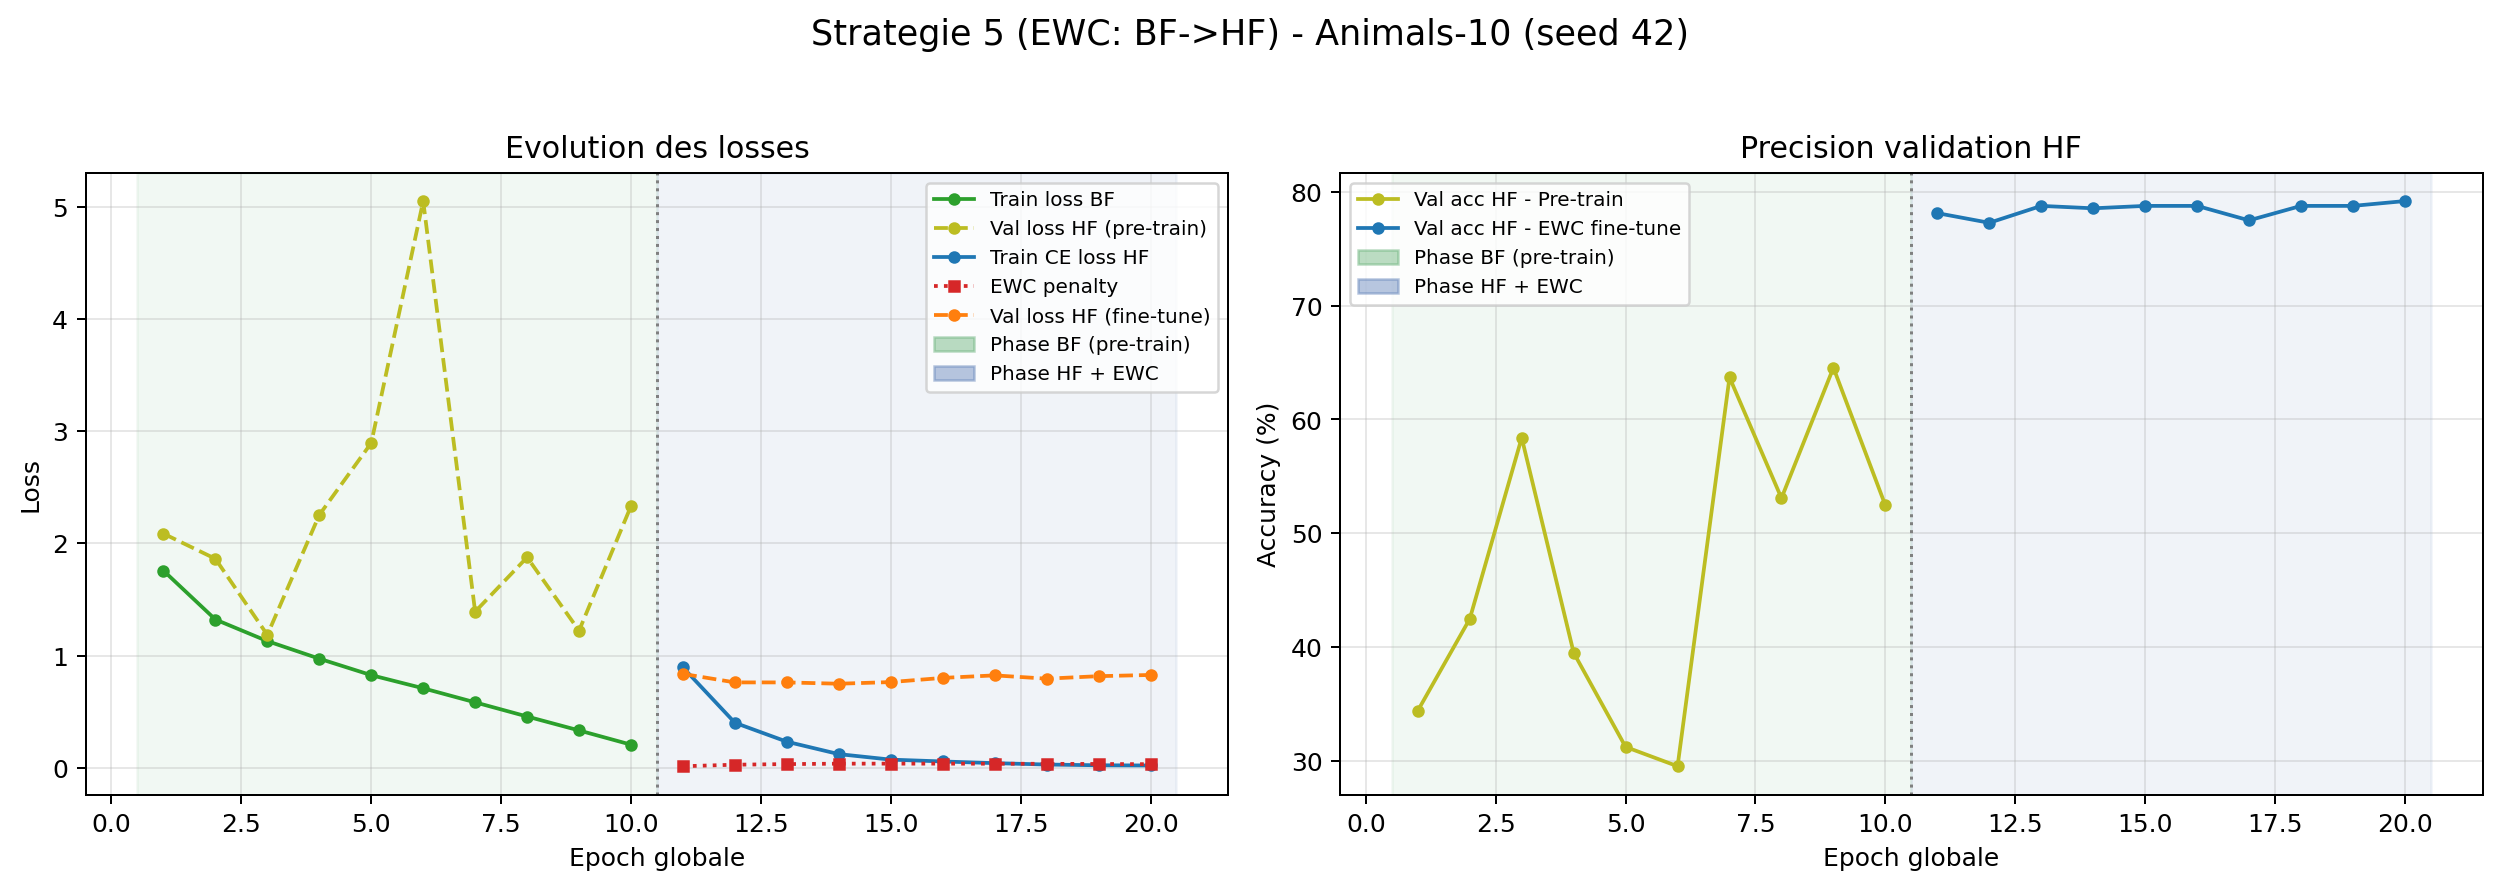
\includegraphics[width=\linewidth]{figures/strategy5_ewc_curves.png}
  \caption{Évolution de la loss et de la précision validation HF pour la Stratégie 4 (EWC) sur \textbf{Animals-10} : pré-entraînement BF puis fine-tuning HF sous pénalité de Fisher.}
  \label{fig:strategy4_ewc_curves}
\end{figure}

% ---- 4.4.3 Comparaison globale ----
\subsection{Comparaison globale des stratégies}

Le tableau de synthèse ci-dessous rassemble \textbf{toutes les approches} (3 baselines + 4 stratégies) sur les \textbf{trois datasets}. Pour chaque dataset, le meilleur score Test HF est mis en évidence.

\vspace{0.6em}
\setlength{\tabcolsep}{4pt}
\renewcommand{\arraystretch}{1.4}
\begin{tabularx}{\linewidth}{L{2.6cm} C{2.45cm} C{2.45cm} C{2.45cm} C{2cm} C{2cm}}
  \arrayrulecolor{midgray}
  \toprule
  \tableheadcolor
  \textbf{Modèle} & \textbf{HF} & \textbf{BF} & \textbf{Mixte} & \textbf{Coût donnée} & \textbf{Coût total} \\
  \midrule
  \multicolumn{6}{l}{\textit{\textbf{Animals-10}}} \\
  \tablerowodd
  BL 1 (HF)    & \res{54,3}{2,2} & \res{27,8}{0,8} & \res{41,1}{1,1} & 23 520 & 470 400 \\
  BL 2 (BF)    & \res{61,3}{6,3} & \res{71,0}{1,5} & \res{66,2}{2,7} & 21 213 & 424 260 \\
  \tablerowodd
  BL 3 (Mixte) & \res{74,0}{3,0} & \res{72,9}{1,1} & \res{73,4}{2,0} & 44 733 & 894 660 \\
  Stratégie 1  & \res{77,7}{0,6} & \res{68,3}{0,5} & \res{73,0}{0,3} & 44 733 & 400 230 \\
  \tablerowodd
  Stratégie 2  & \res{63,8}{5,2} & \res{61,0}{4,2} & \res{62,4}{4,7} & 44 733 & 486 720 \\
  Stratégie 3  & \res{76,5}{0,2} & \res{73,1}{0,1} & \res{74,8}{0,1} & 44 733 & 421 265 \\
  \tablerowodd
  \textbf{Stratégie 4 (EWC)} & \textbf{\res{78,0}{0,3}} & \res{68,8}{0,7} & \res{73,4}{0,4} & 44 733 & \textbf{400 230} \\
  \midrule
  \multicolumn{6}{l}{\textit{\textbf{Imagewoof}}} \\
  \tablerowodd
  BL 1 (HF)    & \res{25,0}{4,1} & \res{22,1}{1,4} & \res{23,5}{2,6} & 8 990  & 179 800 \\
  BL 2 (BF)    & \res{42,7}{2,8} & \res{47,0}{1,6} & \res{44,9}{2,1} & 8 126  & 162 520 \\
  \tablerowodd
  BL 3 (Mixte) & \res{50,3}{2,5} & \res{48,8}{2,3} & \res{49,6}{2,4} & 17 116 & 342 320 \\
  Stratégie 1  & \res{51,0}{1,6} & \res{44,7}{1,3} & \res{47,9}{1,5} & 17 116 & 153 160 \\
  \tablerowodd
  Stratégie 2  & \res{37,5}{0,8} & \res{37,4}{0,3} & \res{37,5}{0,2} & 17 116 & 183 040 \\
  Stratégie 3  & \res{47,5}{1,4} & \res{46,1}{1,1} & \res{46,8}{1,2} & 17 116 & 158 880 \\
  \tablerowodd
  \textbf{Stratégie 4 (EWC)} & \textbf{\res{53,3}{0,7}} & \res{46,8}{0,6} & \res{50,0}{0,6} & 17 116 & \textbf{153 160} \\
  \midrule
  \multicolumn{6}{l}{\textit{\textbf{Intel}}} \\
  \tablerowodd
  BL 1 (HF)    & \res{75,8}{2,2} & \res{47,0}{0,8} & \res{61,4}{1,1} & 14 020 & 280 400 \\
  BL 2 (BF)    & \res{78,7}{2,7} & \res{81,9}{1,4} & \res{80,3}{1,4} & 12 632 & 252 640 \\
  \tablerowodd
  BL 3 (Mixte) & \res{82,8}{1,2} & \res{82,1}{1,2} & \res{82,5}{1,2} & 26 652 & 533 040 \\
  \textbf{Stratégie 1}  & \textbf{\res{86,1}{0,4}} & \res{79,1}{1,4} & \res{82,6}{0,7} & 26 652 & \textbf{238 420} \\
  \tablerowodd
  Stratégie 2  & \res{82,0}{1,0} & \res{79,8}{0,9} & \res{80,9}{0,9} & 26 652 & 291 200 \\
  Stratégie 3  & \res{84,6}{1,0} & \res{82,6}{1,5} & \res{83,6}{1,2} & 26 652 & 250 880 \\
  \tablerowodd
  Stratégie 4 (EWC) & \res{85,8}{0,4} & \res{80,0}{0,9} & \res{82,9}{0,6} & 26 652 & 238 420 \\
  \bottomrule
\end{tabularx}
\setlength{\tabcolsep}{6pt}

\vspace{0.8em}
Lectures clés du tableau de synthèse :

\begin{itemize}
  \item \textbf{EWC, meilleure stratégie pour l'objectif HF} : EWC obtient le meilleur Test HF sur Animals-10 (78,0\,\%) et Imagewoof (53,3\,\%), et talonne la Stratégie 1 sur Intel (85,8 vs 86,1\,\%) — le tout au \textbf{coût le plus bas} (identique à S1) et avec une excellente stabilité.
  \item \textbf{EWC domine la Stratégie 1} : à pipeline et coût identiques, EWC est supérieur ou égal à S1 en HF \emph{et} en BF sur les trois datasets : la pénalité de Fisher est un ajout « gratuit » bénéfique.
  \item \textbf{Curriculum, meilleur équilibre} : la Stratégie 3 offre la meilleure rétention BF et la meilleure stabilité, au prix d'un HF légèrement inférieur à EWC/S1.
  \item \textbf{Toutes les stratégies orientées HF battent les baselines à coût réduit} : S1, S3 et S4 dépassent la borne supérieure BL 3 sur Test HF (Animals-10 et Intel) tout en divisant le coût total par environ deux ; seule la Stratégie 2 reste en retrait.
\end{itemize}

% ---- 4.4.4 Analyse ----
\subsection{Analyse : ce qui a marché, ce qui a moins marché, et enseignements}

\begin{itemize}
  \item \textbf{Ce qui a bien marché} : la pénalité de Fisher atteint son objectif — spécialiser le modèle sur HF \emph{sans} effondrer la robustesse BF — ce qui fait d'EWC la meilleure approche pour la cible HF, à coût minimal.
  \item \textbf{Gain le plus net sur le fine-grained} : c'est sur Imagewoof (faible volume HF) que l'apport d'EWC sur la Stratégie 1 est le plus marqué ($+2,3$ points HF), là où la protection des acquis BF compte le plus.
  \item \textbf{Limite} : EWC ajoute deux hyperparamètres ($\lambda$, nombre d'échantillons Fisher) et un coût de calcul de la matrice de Fisher ; le réglage de $\lambda$ conditionne l'équilibre spécialisation/rétention.
  \item \textbf{Leçon principale} : ancrer explicitement les poids importants pour le domaine bon marché est un levier simple et efficace pour pousser la performance HF sans payer la robustesse BF.
\end{itemize}

\begin{decisionbox}
  \textbf{Conclusion (Stratégie 4) — bilan des stratégies :} pour l'objectif HF prioritaire à coût réduit, le classement qui se dégage est \textbf{EWC $\gtrsim$ Stratégie 1 $>$ Curriculum $>$ Co-training}, toutes nettement meilleures que les baselines à coût total équivalent ou inférieur. \textbf{EWC} est recommandé lorsque la performance HF prime ; le \textbf{Curriculum} lorsqu'un équilibre HF/BF robuste est recherché. La phase suivante (optimisation Optuna) cherchera à raffiner les hyperparamètres de chacune de ces stratégies.
\end{decisionbox}

% ============================================================
%  CHAPITRE — Optimisation des hyperparamètres (Optuna)
% ============================================================
\chapter{Optimisation des hyperparamètres (Optuna)}

Les stratégies du chapitre précédent ont été évaluées avec des hyperparamètres choisis par l'intuition et l'expérience (taux d'apprentissage, nombre d'époques, poids de perte, etc.). Cette configuration « de base » n'est pas nécessairement optimale. Ce chapitre cherche, pour chaque stratégie et chaque dataset, une configuration améliorée à l'aide de la bibliothèque d'optimisation \textbf{Optuna}~\cite{akiba2019optuna}.

\section{Méthode}

Optuna explore automatiquement l'espace des hyperparamètres à l'aide d'un échantillonneur bayésien (TPE, \textit{Tree-structured Parzen Estimator}) qui concentre progressivement la recherche sur les régions prometteuses. Le protocole retenu est le suivant :

\begin{itemize}
  \item \textbf{Objectif optimisé} : la précision de \textbf{validation HF} (cohérente avec l'objectif HF prioritaire du projet) ;
  \item \textbf{Budget} : $n_{trials}=20$ essais par stratégie et par dataset ;
  \item \textbf{Évaluation finale} : la meilleure configuration trouvée est ré-entraînée et évaluée selon le \emph{même} protocole multi-graines que les versions de base (moyenne $\pm$ écart-type), pour une comparaison équitable.
\end{itemize}

\vspace{0.4em}
Les espaces de recherche, propres à chaque stratégie, portent sur ses hyperparamètres les plus sensibles :

\vspace{0.6em}
\renewcommand{\arraystretch}{1.4}
\begin{tabularx}{\linewidth}{L{3cm} L{12.5cm}}
  \arrayrulecolor{midgray}
  \toprule
  \tableheadcolor
  \textbf{Stratégie} & \textbf{Hyperparamètres explorés (et plages)} \\
  \midrule
  \tablerowodd
  S1 Transfer & $lr_{pretrain}$, $lr_{finetune}$ (échelle log $\sim$[$10^{-5}$, $5\!\cdot\!10^{-3}$]), époques BF et HF ($\sim$[5, 15]) \\
  S2 Co-training & $lr$, ratio HF par batch ($\sim$[0,10\,;\,0,40]), poids de perte $w_{HF}$ ($\sim$[1\,;\,3]) et $w_{BF}$ ($\sim$[0,4\,;\,1,4]) \\
  \tablerowodd
  S3 Curriculum & $lr$, époques par palier ($\sim$[4, 8]), proportions HF intermédiaires $ratio_{mid1}$ et $ratio_{mid2}$ \\
  S4 EWC & $lr_{pretrain}$, $lr_{finetune}$, force du rappel $\lambda$ (échelle log $\sim$[10, 1000]), époques BF et HF \\
  \bottomrule
\end{tabularx}

\section{Résultats}

Le tableau ci-dessous compare, sur la métrique cible Test HF, chaque stratégie dans sa version de base et sa version optimisée par Optuna, pour les trois datasets.

\vspace{0.6em}
\setlength{\tabcolsep}{4pt}
\renewcommand{\arraystretch}{1.4}
\begin{tabularx}{\linewidth}{L{2.4cm} L{2.4cm} C{2.7cm} C{2.7cm} C{2.2cm}}
  \arrayrulecolor{midgray}
  \toprule
  \tableheadcolor
  \textbf{Stratégie} & \textbf{Dataset} & \textbf{HF (base)} & \textbf{HF (+Optuna)} & \textbf{$\Delta$ HF} \\
  \midrule
  \multicolumn{5}{l}{\textit{\textbf{S1 — Transfer Learning}}} \\
  \tablerowodd
  & Animals-10 & \res{77,7}{0,6} & \res{78,1}{0,1} & $+0,4$ \\
  & Imagewoof  & \res{51,0}{1,6} & \res{49,8}{1,1} & $-1,2$ \\
  \tablerowodd
  & Intel      & \res{86,1}{0,4} & \res{86,0}{0,4} & $-0,1$ \\
  \midrule
  \multicolumn{5}{l}{\textit{\textbf{S2 — Co-training pondéré}}} \\
  \tablerowodd
  & Animals-10 & \res{63,8}{5,2} & \textbf{\res{73,2}{2,1}} & $\mathbf{+9,4}$ \\
  & Imagewoof  & \res{37,5}{0,8} & \res{42,2}{0,5} & $+4,7$ \\
  \tablerowodd
  & Intel      & \res{82,0}{1,0} & \res{82,0}{1,2} & $0,0$ \\
  \midrule
  \multicolumn{5}{l}{\textit{\textbf{S3 — Curriculum Learning}}} \\
  \tablerowodd
  & Animals-10 & \res{76,5}{0,2} & \res{77,0}{0,6} & $+0,5$ \\
  & Imagewoof  & \res{47,5}{1,4} & \textbf{\res{52,8}{0,4}} & $\mathbf{+5,3}$ \\
  \tablerowodd
  & Intel      & \res{84,6}{1,0} & \res{86,0}{0,8} & $+1,4$ \\
  \midrule
  \multicolumn{5}{l}{\textit{\textbf{S4 — EWC}}} \\
  \tablerowodd
  & Animals-10 & \res{78,0}{0,3} & \res{76,0}{0,6} & $-2,0$ \\
  & Imagewoof  & \res{53,3}{0,7} & \res{53,4}{1,5} & $+0,1$ \\
  \tablerowodd
  & Intel      & \res{85,8}{0,4} & \res{82,0}{0,4} & $-3,8$ \\
  \bottomrule
\end{tabularx}
\setlength{\tabcolsep}{6pt}

\begin{hypothesebox}[Lecture des figures]
  Les figures de ce rapport sont générées par le code d'analyse, qui utilise une numérotation interne : la stratégie \textbf{EWC y est étiquetée « S5 »} et le \textbf{curriculum « S3 »}. Elles correspondent respectivement aux \textbf{Stratégies 4 et 3} du texte ; les Stratégies 1 (Transfer) et 2 (Co-training) gardent la même numérotation.
\end{hypothesebox}

\begin{figure}[htbp]
  \centering
  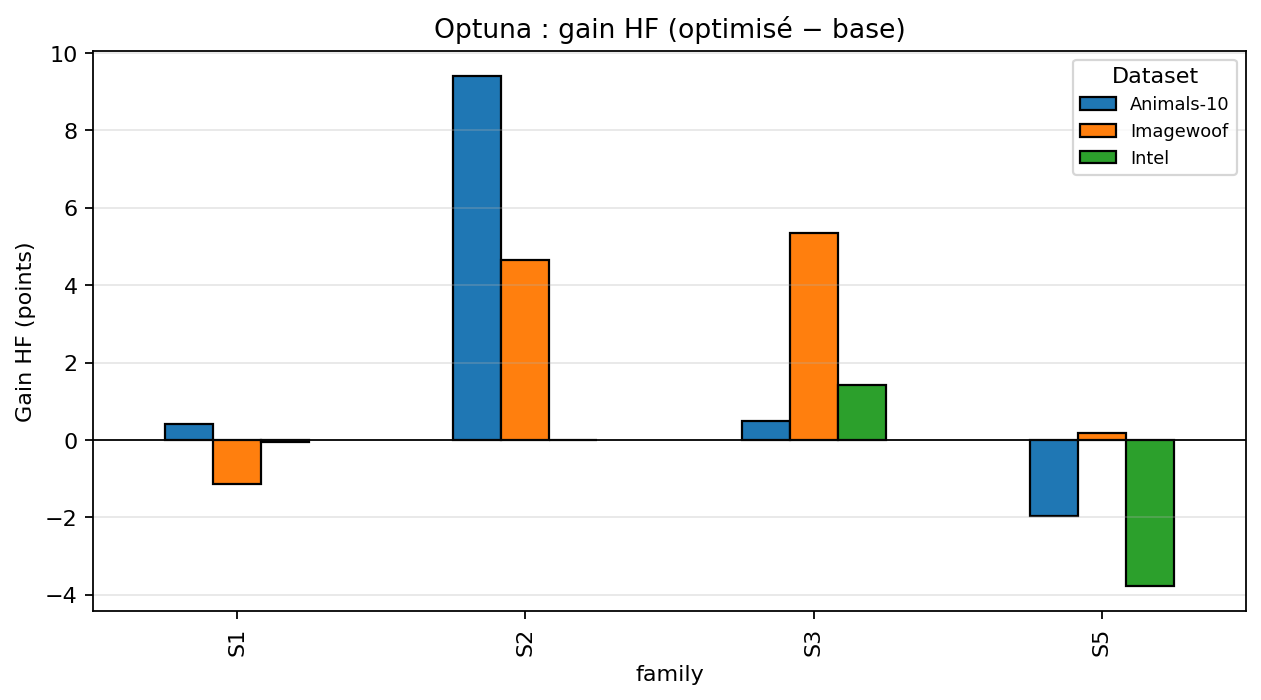
\includegraphics[width=\linewidth]{figures/optuna_gains.png}
  \caption{Gains de précision Test HF apportés par l'optimisation Optuna (version optimisée $-$ version de base), par stratégie et par dataset. (Légende : « S5 » = EWC = Stratégie 4 ; « S3 » = Curriculum = Stratégie 3.)}
  \label{fig:optuna_gains}
\end{figure}

\subsection{Configurations retenues}

Le tableau ci-dessous récapitule les meilleurs hyperparamètres trouvés par Optuna pour chaque stratégie et chaque dataset.

\vspace{0.4em}
\setlength{\tabcolsep}{4pt}
\renewcommand{\arraystretch}{1.35}
\begin{tabularx}{\linewidth}{L{1.7cm} L{2cm} X}
  \arrayrulecolor{midgray}
  \toprule
  \tableheadcolor
  \textbf{Stratégie} & \textbf{Dataset} & \textbf{Hyperparamètres retenus} \\
  \midrule
  \multirow{3}{*}{S1} & Animals-10 & $lr_{pre}\!=\!1{,}1\!\cdot\!10^{-3}$, $lr_{ft}\!=\!4{,}1\!\cdot\!10^{-4}$, époques BF/HF $=$ 9/13 \\
   & Imagewoof & $lr_{pre}\!=\!4{,}1\!\cdot\!10^{-4}$, $lr_{ft}\!=\!1{,}6\!\cdot\!10^{-5}$, époques BF/HF $=$ 12/9 \\
   & Intel & $lr_{pre}\!=\!1{,}7\!\cdot\!10^{-3}$, $lr_{ft}\!=\!1{,}9\!\cdot\!10^{-5}$, époques BF/HF $=$ 8/9 \\
  \midrule
  \multirow{3}{*}{S2} & Animals-10 & $lr\!=\!8{,}5\!\cdot\!10^{-4}$, ratio HF $=$ 0,16, $w_{HF}\!=\!2{,}2$, $w_{BF}\!=\!1{,}0$ \\
   & Imagewoof & $lr\!=\!3{,}2\!\cdot\!10^{-3}$, ratio HF $=$ 0,10, $w_{HF}\!=\!2{,}7$, $w_{BF}\!=\!0{,}88$ \\
   & Intel & $lr\!=\!2{,}2\!\cdot\!10^{-3}$, ratio HF $=$ 0,23, $w_{HF}\!=\!2{,}2$, $w_{BF}\!=\!1{,}4$ \\
  \midrule
  \multirow{3}{*}{S3} & Animals-10 & $lr\!=\!5{,}6\!\cdot\!10^{-4}$, époques/palier $=$ 8, ratios HF $=$ 0,32 / 0,69 \\
   & Imagewoof & $lr\!=\!9{,}4\!\cdot\!10^{-4}$, époques/palier $=$ 8, ratios HF $=$ 0,22 / 0,83 \\
   & Intel & $lr\!=\!8{,}2\!\cdot\!10^{-4}$, époques/palier $=$ 7, ratios HF $=$ 0,16 / 0,66 \\
  \midrule
  \multirow{3}{*}{S4 (EWC)} & Animals-10 & $lr_{pre}\!=\!1{,}7\!\cdot\!10^{-3}$, $lr_{ft}\!=\!1{,}9\!\cdot\!10^{-5}$, $\lambda\!=\!38$, époques BF/HF $=$ 9/10 \\
   & Imagewoof & $lr_{pre}\!=\!1{,}6\!\cdot\!10^{-3}$, $lr_{ft}\!=\!2{,}2\!\cdot\!10^{-5}$, $\lambda\!=\!13$, époques BF/HF $=$ 15/15 \\
   & Intel & $lr_{pre}\!=\!2{,}3\!\cdot\!10^{-4}$, $lr_{ft}\!=\!4{,}1\!\cdot\!10^{-5}$, $\lambda\!=\!112$, époques BF/HF $=$ 9/8 \\
  \bottomrule
\end{tabularx}
\setlength{\tabcolsep}{6pt}

\vspace{0.4em}
On notera que, pour EWC, Optuna sélectionne systématiquement une force de rappel $\lambda$ \textbf{bien inférieure} à la valeur de base ($\lambda=400$) : entre 13 et 112 selon le dataset. Ce relâchement de la contrainte favorise la précision de validation mais explique la dégradation observée en test (cf. analyse ci-dessous).

\section{Analyse}

\begin{itemize}
  \item \textbf{Optuna aide surtout les stratégies instables ou faibles} : les gains les plus nets concernent S2 (co-training) sur Animals-10 ($+9,4$ points, avec en prime une variance divisée par $\approx$2,5 : $\pm$5,2~$\rightarrow$~$\pm$2,1) et S3 (curriculum) sur Imagewoof ($+5,3$ points). Là où la configuration de base était sous-optimale, la recherche bayésienne récupère une marge importante.
  \item \textbf{Peu de marge sur les stratégies déjà fortes et stables} : pour S1 et EWC, dont les versions de base sont déjà excellentes et très stables, le gain est faible, nul, voire \textbf{négatif} sur Test HF. EWC se dégrade même nettement sur Animals-10 ($-2,0$) et Intel ($-3,8$) : Optuna a sélectionné un rappel de Fisher beaucoup plus faible ($\lambda\approx38$ et $112$ contre $400$ en base), bénéfique en \emph{validation} mais pénalisant en \emph{test}, signe d'un léger sur-ajustement à l'ensemble de validation avec un budget de seulement 20 essais.
  \item \textbf{Le coût de calcul peut augmenter} : Optuna optimisant la seule précision HF, il choisit parfois davantage d'époques HF, ce qui alourdit le coût total (ex. S3 sur Animals-10 : 421\,k~$\rightarrow$~658\,k CA). Le gain de précision doit donc se lire conjointement au coût.
  \item \textbf{Meilleures configurations après optimisation} : Animals-10 — S1+Optuna (78,1\,\%) ; Imagewoof — EWC+Optuna et Curriculum+Optuna ($\approx$53 et 52,8\,\%) ; Intel — S1+Optuna et Curriculum+Optuna ($\approx$86\,\%).
\end{itemize}

\begin{decisionbox}
  \textbf{Conclusion (Optuna) :} l'optimisation automatique est précieuse pour \textbf{récupérer le potentiel des stratégies mal réglées} (S2, S3), mais apporte peu — et peut nuire — aux stratégies déjà robustes (S1, EWC) sous un budget restreint. Un budget d'essais plus large et une fonction objectif intégrant le coût (optimisation multi-objectif) sont les pistes naturelles d'amélioration.
\end{decisionbox}


% ============================================================
%  CHAPITRE — Analyses transversales
% ============================================================
\chapter{Analyses de robustesse et de sensibilité}

Au-delà de la précision moyenne, deux questions déterminent la valeur pratique d'une stratégie : comment se comporte-t-elle face à des données \emph{plus} dégradées que prévu (robustesse) ? et ses conclusions économiques tiennent-elles si l'on modifie l'hypothèse de coût (sensibilité) ?

\section{Robustesse face à la dégradation}

\subsection{Protocole}

Chaque modèle entraîné (les 7 modèles : 3 baselines + 4 stratégies) est évalué sur des versions du jeu de test \textbf{progressivement dégradées}~\cite{hendrycks2019}, selon deux balayages indépendants :

\begin{itemize}
  \item \textbf{Perte de résolution} : sous-échantillonnage croissant $224 \rightarrow 128 \rightarrow 96 \rightarrow 64 \rightarrow 48 \rightarrow 32$ px (bruit fixé à $\sigma=0{,}15$) ;
  \item \textbf{Bruit gaussien} : $\sigma = 0 \rightarrow 0{,}05 \rightarrow 0{,}1 \rightarrow 0{,}15 \rightarrow 0{,}25 \rightarrow 0{,}35$ (résolution fixée à 64~px).
\end{itemize}

On mesure la précision sur le domaine HF à chaque niveau. Une bonne robustesse se traduit par une décroissance \emph{lente} de la précision lorsque la dégradation augmente.

\begin{figure}[htbp]
  \centering
  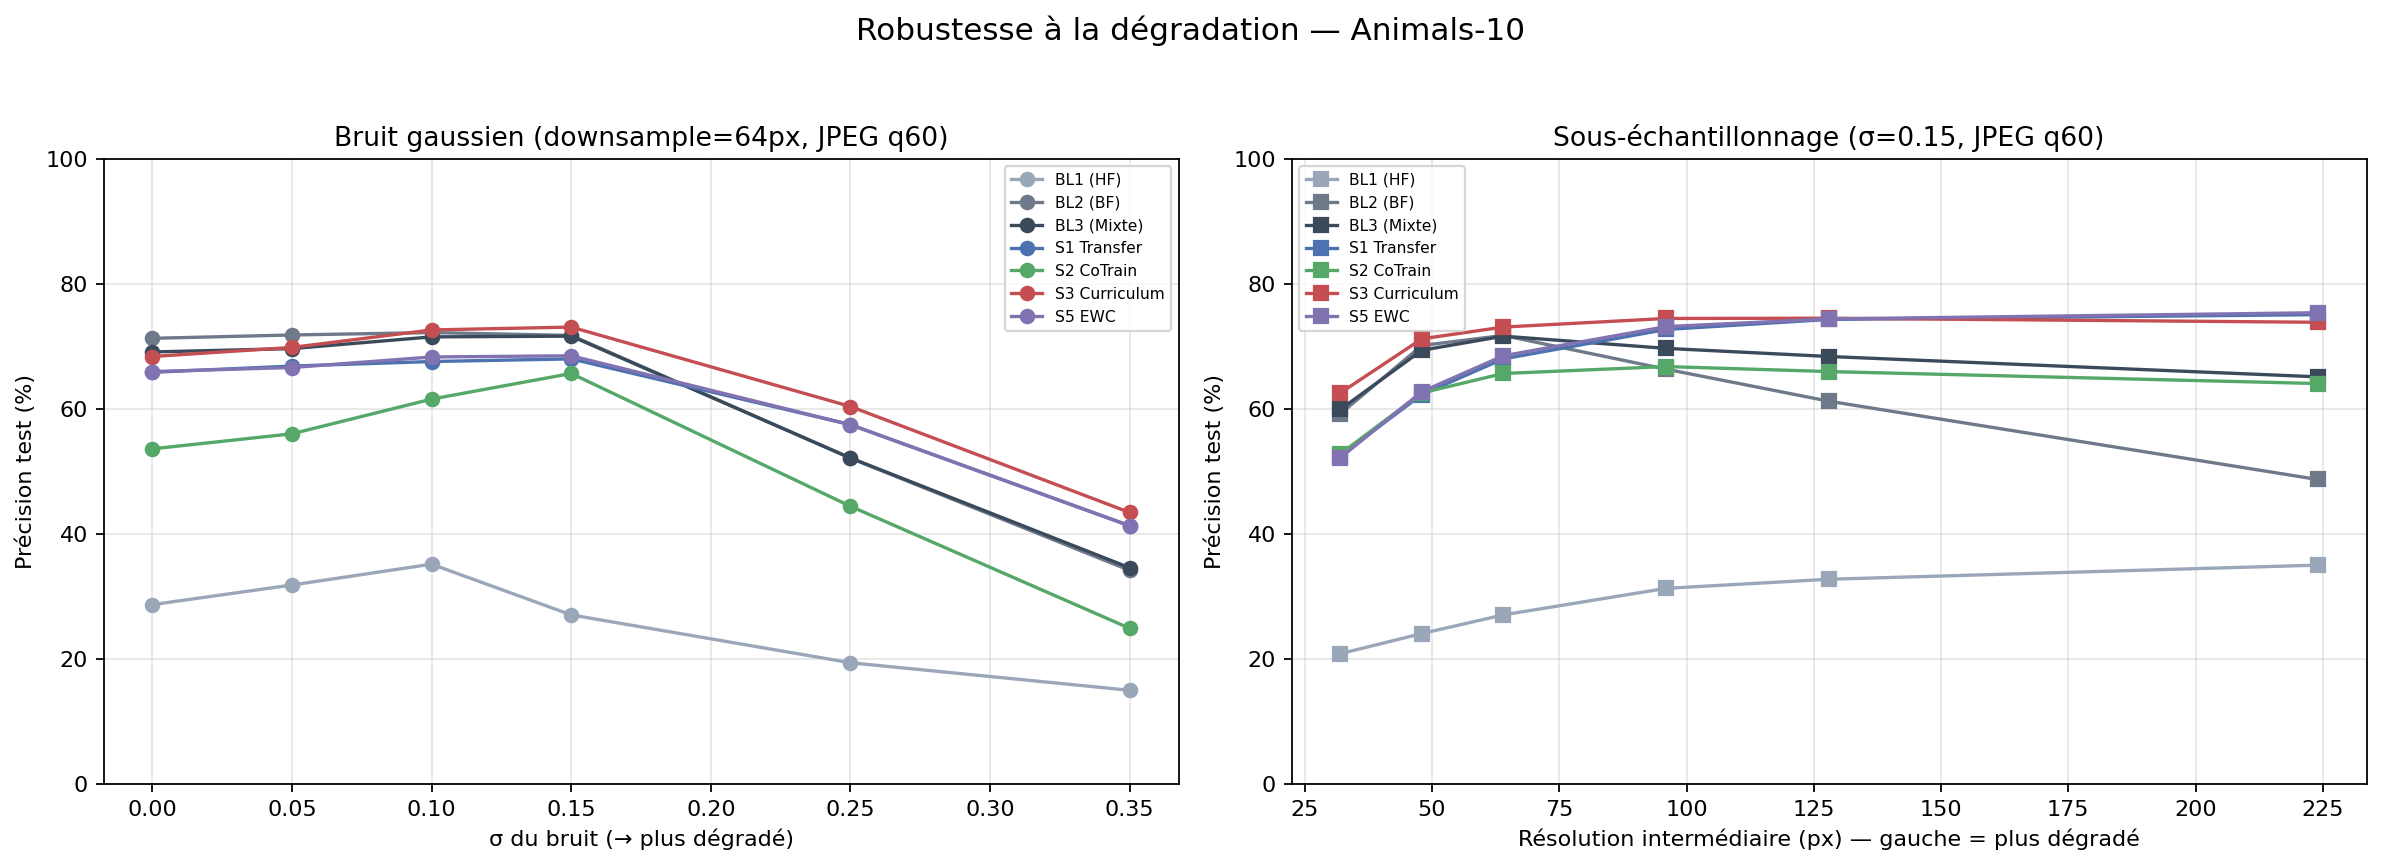
\includegraphics[width=\linewidth]{figures/robustness_degradation_animals10.png}
  \caption{Robustesse sur \textbf{Animals-10} : précision en fonction de la perte de résolution (gauche) et du bruit gaussien (droite), pour les 7 modèles. (Légende : « S5 » = EWC = Stratégie 4 ; « S3 » = Curriculum = Stratégie 3.)}
  \label{fig:robustness_animals}
\end{figure}

\begin{figure}[htbp]
  \centering
  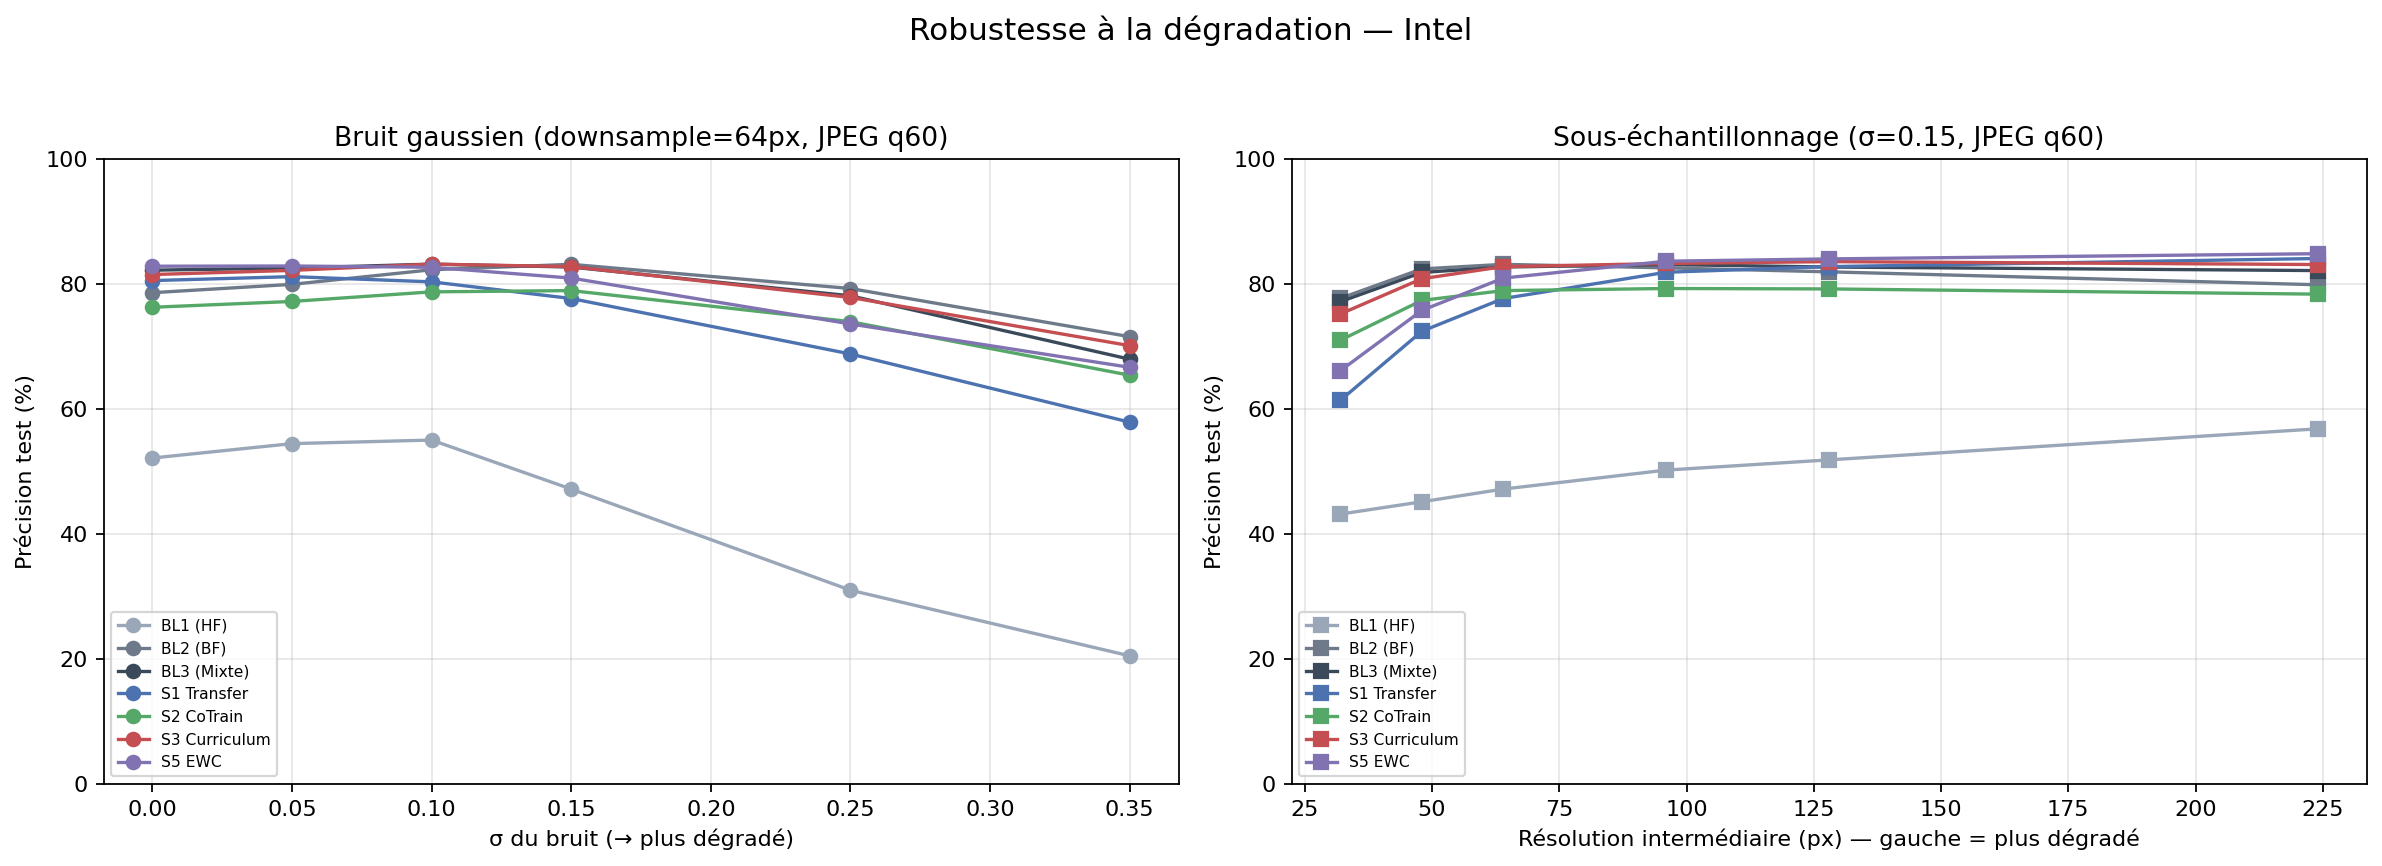
\includegraphics[width=\linewidth]{figures/robustness_degradation_intel.png}
  \caption{Robustesse sur \textbf{Intel} : précision en fonction de la perte de résolution et du bruit gaussien.}
  \label{fig:robustness_intel}
\end{figure}

\begin{figure}[htbp]
  \centering
  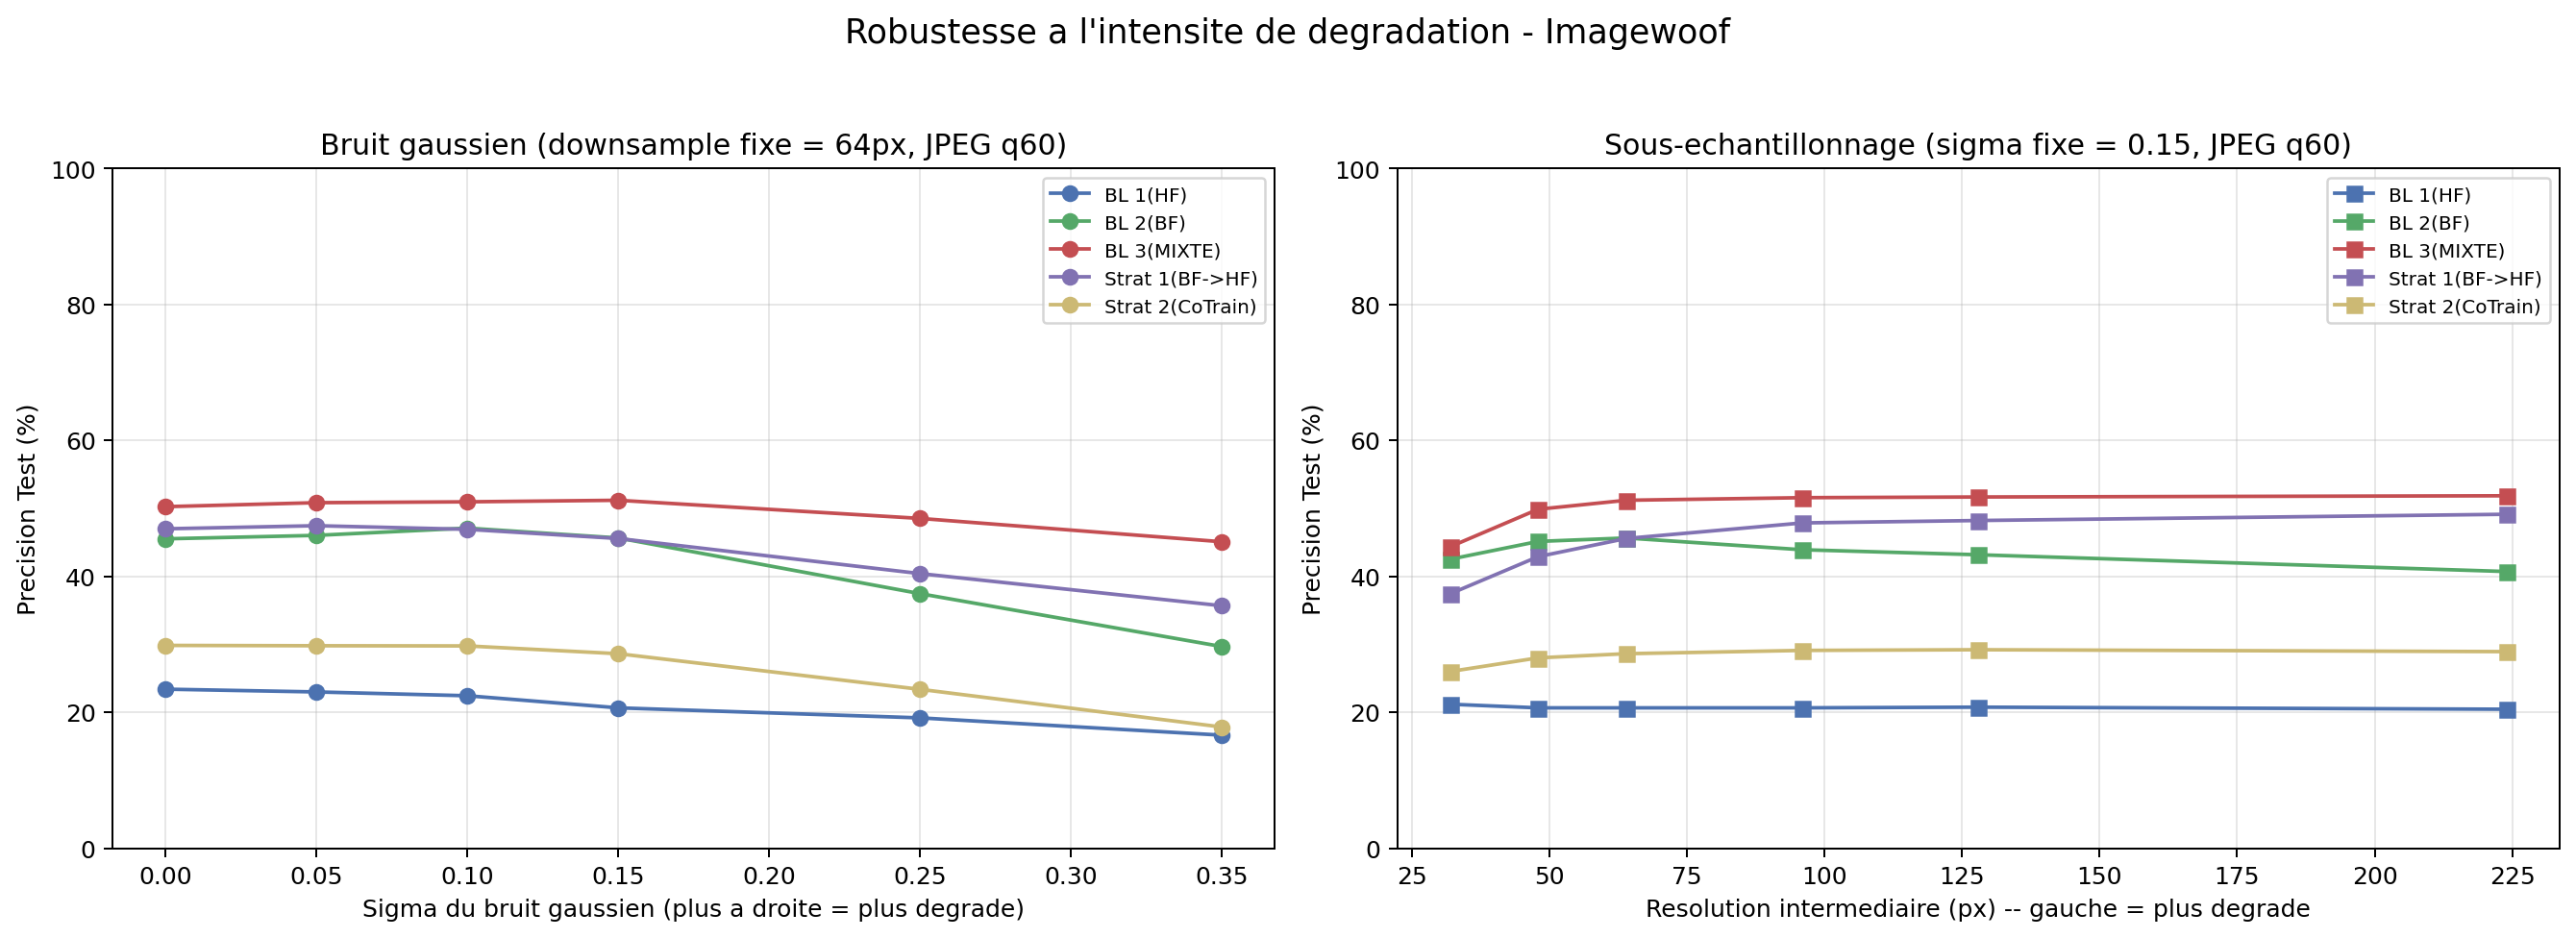
\includegraphics[width=\linewidth]{figures/robustness_degradation_imagewoof.png}
  \caption{Robustesse sur \textbf{Imagewoof} : précision en fonction de la perte de résolution et du bruit gaussien.}
  \label{fig:robustness_imagewoof}
\end{figure}

\subsection{Résultats et enseignements}

\begin{itemize}
  \item \textbf{La baseline Premium (BL 1) s'effondre} : entraînée sur HF uniquement, elle chute le plus vite sur les deux axes (sur Animals-10, de 53\,\% à 21\,\% en résolution et à 15\,\% en bruit). C'est le modèle le moins robuste, confirmant le \textit{domain shift}.
  \item \textbf{La baseline Low-Cost (BL 2) est très robuste à la perte de résolution} : entraînée sur des images BF à 64~px, sa précision est quasi insensible au sous-échantillonnage (sur Intel, elle \emph{augmente} même de 76 à 80\,\% autour de 64~px) ; en revanche elle reste fragile au \textbf{bruit fort} ($\sigma=0{,}35$).
  \item \textbf{Un compromis précision-propre / robustesse apparaît} : S1 et EWC offrent la meilleure précision sur données propres mais déclinent plus rapidement sous forte dégradation (sur Animals-10, S1 passe de 78 à 53\,\% en résolution extrême). Ils sont spécialisés HF.
  \item \textbf{Le Curriculum (S3) est la stratégie la plus robuste} : sur les trois datasets, c'est elle qui conserve la \textbf{meilleure précision minimale} sous dégradation extrême (Animals-10 : 63\,\% en résolution et 43\,\% en bruit, contre $\approx$52 et 41\,\% pour S1/EWC). Ce résultat est cohérent avec sa meilleure rétention BF : la transition douce BF~$\rightarrow$~HF lui a conservé des représentations robustes aux basses fréquences.
\end{itemize}

\begin{decisionbox}
  \textbf{Conclusion (robustesse) :} il existe un arbitrage clair. Pour une \textbf{précision maximale sur données propres}, EWC/S1 restent les meilleurs. Mais si le déploiement implique des données \textbf{encore plus dégradées} que l'entraînement, le \textbf{Curriculum} est le choix le plus sûr, et la baseline BF reste imbattable face à la seule perte de résolution.
\end{decisionbox}

\section{Sensibilité au ratio de coût HF:BF}

\subsection{Protocole}

Le modèle de coût repose sur un ratio de coût unitaire HF:BF calibré à \textbf{10:1} (cf. la définition de la métrique de coût au chapitre Fondation). Ce choix est défendable mais arbitraire. Cette analyse \textit{post-hoc} recalcule le coût d'acquisition de chaque modèle pour une gamme de ratios — \textbf{2, 5, 10, 20, 50} — et détermine, à chaque ratio, le modèle le plus \textbf{efficient} (meilleur rapport précision HF / coût donnée). L'objectif est de savoir si le classement économique est \textbf{robuste} au choix du ratio.

\begin{figure}[htbp]
  \centering
  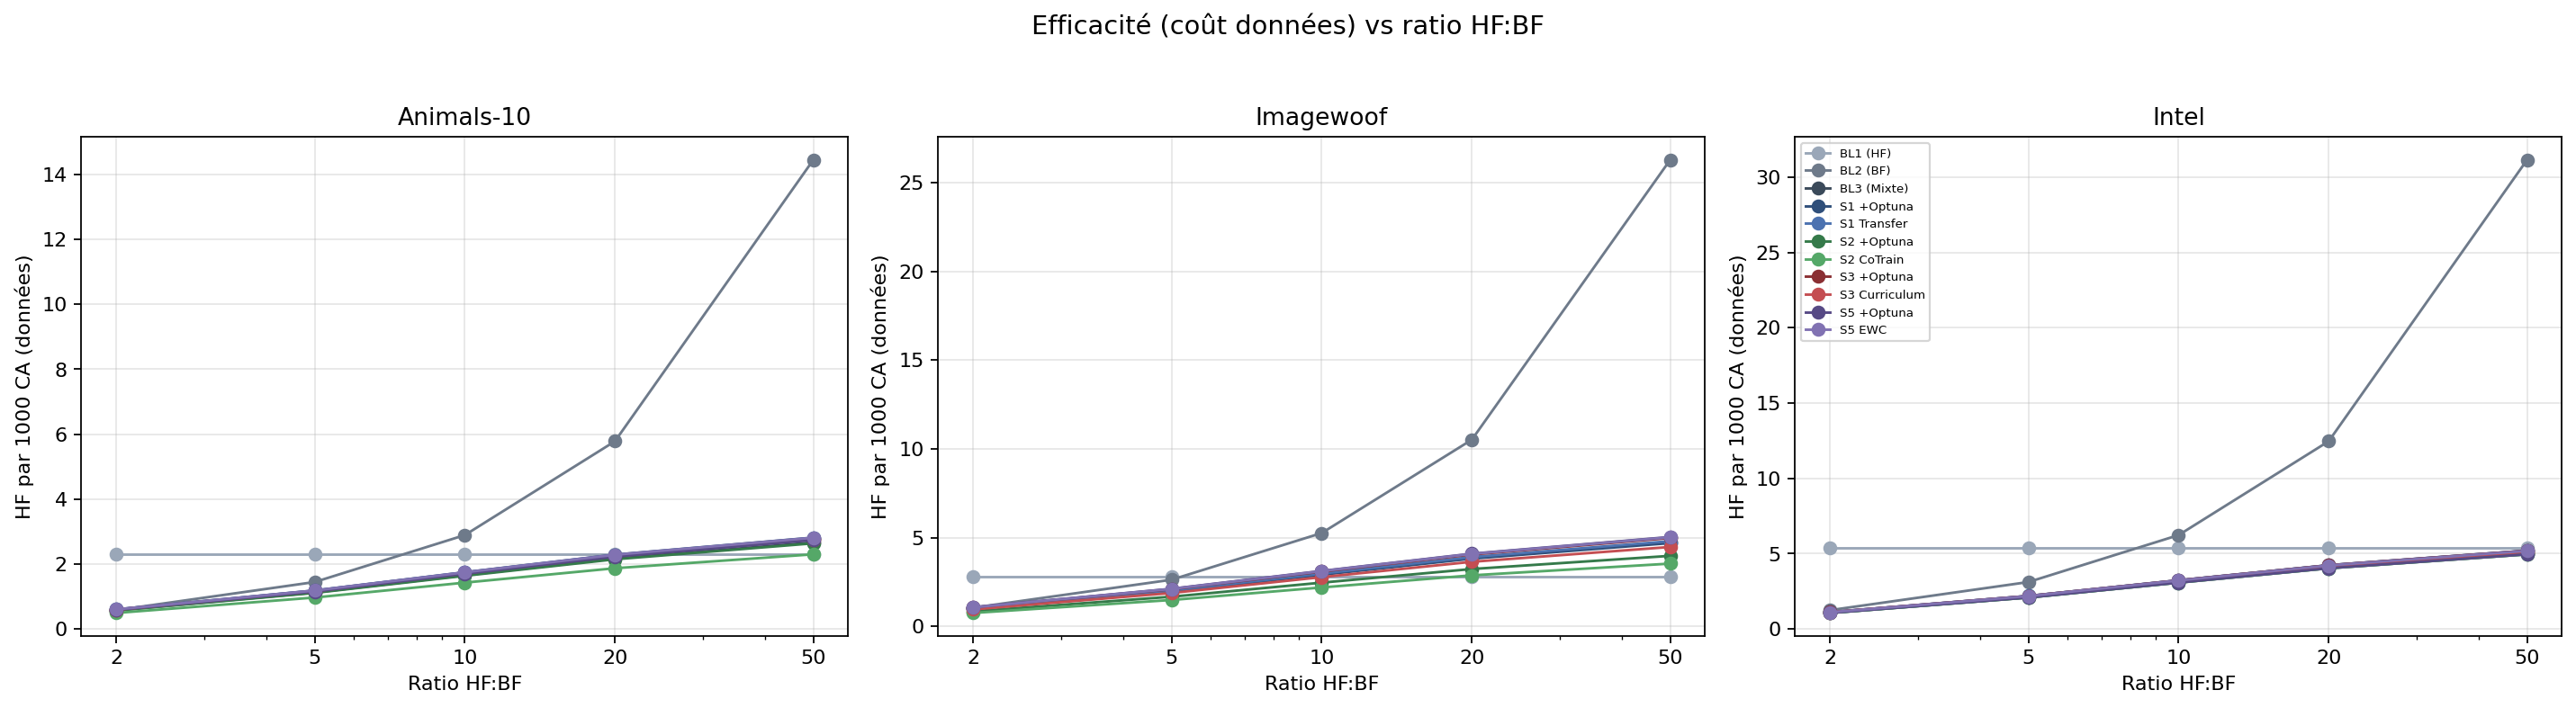
\includegraphics[width=\linewidth]{figures/ratio_efficacite_donnees.png}
  \caption{Efficience (précision HF par unité de coût donnée) en fonction du ratio de coût HF:BF, par modèle et par dataset.}
  \label{fig:ratio_sensitivity}
\end{figure}

\subsection{Résultats et enseignements}

\begin{itemize}
  \item \textbf{Le classement économique n'est PAS robuste au ratio} : le modèle le plus efficient \emph{change} selon le ratio supposé, et ce de manière identique sur les trois datasets. Lorsque le HF est \textbf{bon marché} (ratios 2 et 5), la baseline \textbf{Premium (BL 1)} est la plus efficiente ; lorsque le HF devient \textbf{coûteux} (ratios 10, 20, 50), la baseline \textbf{Low-Cost (BL 2)} domine.
  \item \textbf{Interprétation} : ce basculement est mécanique — plus le HF est cher, plus il devient avantageux de s'appuyer sur le volume BF. Aucune approche n'est universellement la plus économique : la « meilleure » dépend de l'hypothèse de coût.
  \item \textbf{Mais l'objectif du projet reste tranché} : ce critère mesure l'\emph{efficience} (précision par CA), pas la \emph{performance absolue}. Or l'objectif est la \textbf{précision HF maximale}, et à ce titre — au ratio calibré 10:1 — les stratégies multi-fidélité (S1, EWC, Curriculum) dominent largement les baselines en précision absolue, pour un coût total réduit de moitié (cf. synthèse globale).
\end{itemize}

\begin{decisionbox}
  \textbf{Conclusion (sensibilité) :} la hiérarchie en \emph{efficience pure} dépend du ratio de coût et n'est donc pas robuste ; il faut expliciter l'hypothèse de coût pour comparer. En revanche, la supériorité des stratégies multi-fidélité en \emph{précision HF absolue} est, elle, robuste et constitue le résultat central du travail.
\end{decisionbox}


% ============================================================
%  CHAPITRE — Synthèse globale
% ============================================================
\chapter{Synthèse globale et comparaison transversale}

Ce chapitre rassemble les enseignements de toutes les expériences précédentes pour dégager une vue d'ensemble : quelle stratégie privilégier, pour quel objectif, et avec quelle confiance ?

\section{Bilan de performance}

En croisant les trois datasets, le multi-graines et les analyses transversales, le classement sur l'\textbf{objectif HF prioritaire} est nettement établi :

\begin{quote}
\centering
\textbf{EWC $\gtrsim$ Transfer Learning (S1) $>$ Curriculum (S3) $>$ Co-training (S2) $\ggg$ baselines}
\end{quote}

\begin{itemize}
  \item \textbf{EWC et Transfer Learning} se partagent la première place en précision HF (meilleurs scores sur les trois datasets), avec une excellente stabilité (écart-type $<1$ point). EWC l'emporte généralement de peu grâce à une meilleure rétention BF, à coût identique.
  \item \textbf{Le Curriculum} suit de près en précision, mais devient le meilleur choix dès que la \textbf{robustesse} et l'\textbf{équilibre HF/BF} priment (cf. chapitre précédent).
  \item \textbf{Le Co-training} est en retrait : instable et sensible au volume HF, il n'est jamais en tête (mais l'optimisation Optuna le rend nettement plus compétitif).
  \item \textbf{Toutes les stratégies orientées HF battent la borne supérieure Mixte (BL 3)} sur Test HF (Animals-10 et Intel), tout en \textbf{divisant le coût total par environ deux}, à coût d'acquisition identique. C'est le résultat clé : on atteint — et dépasse — la performance du mélange naïf coûteux, pour beaucoup moins cher.
\end{itemize}

\begin{figure}[htbp]
  \centering
  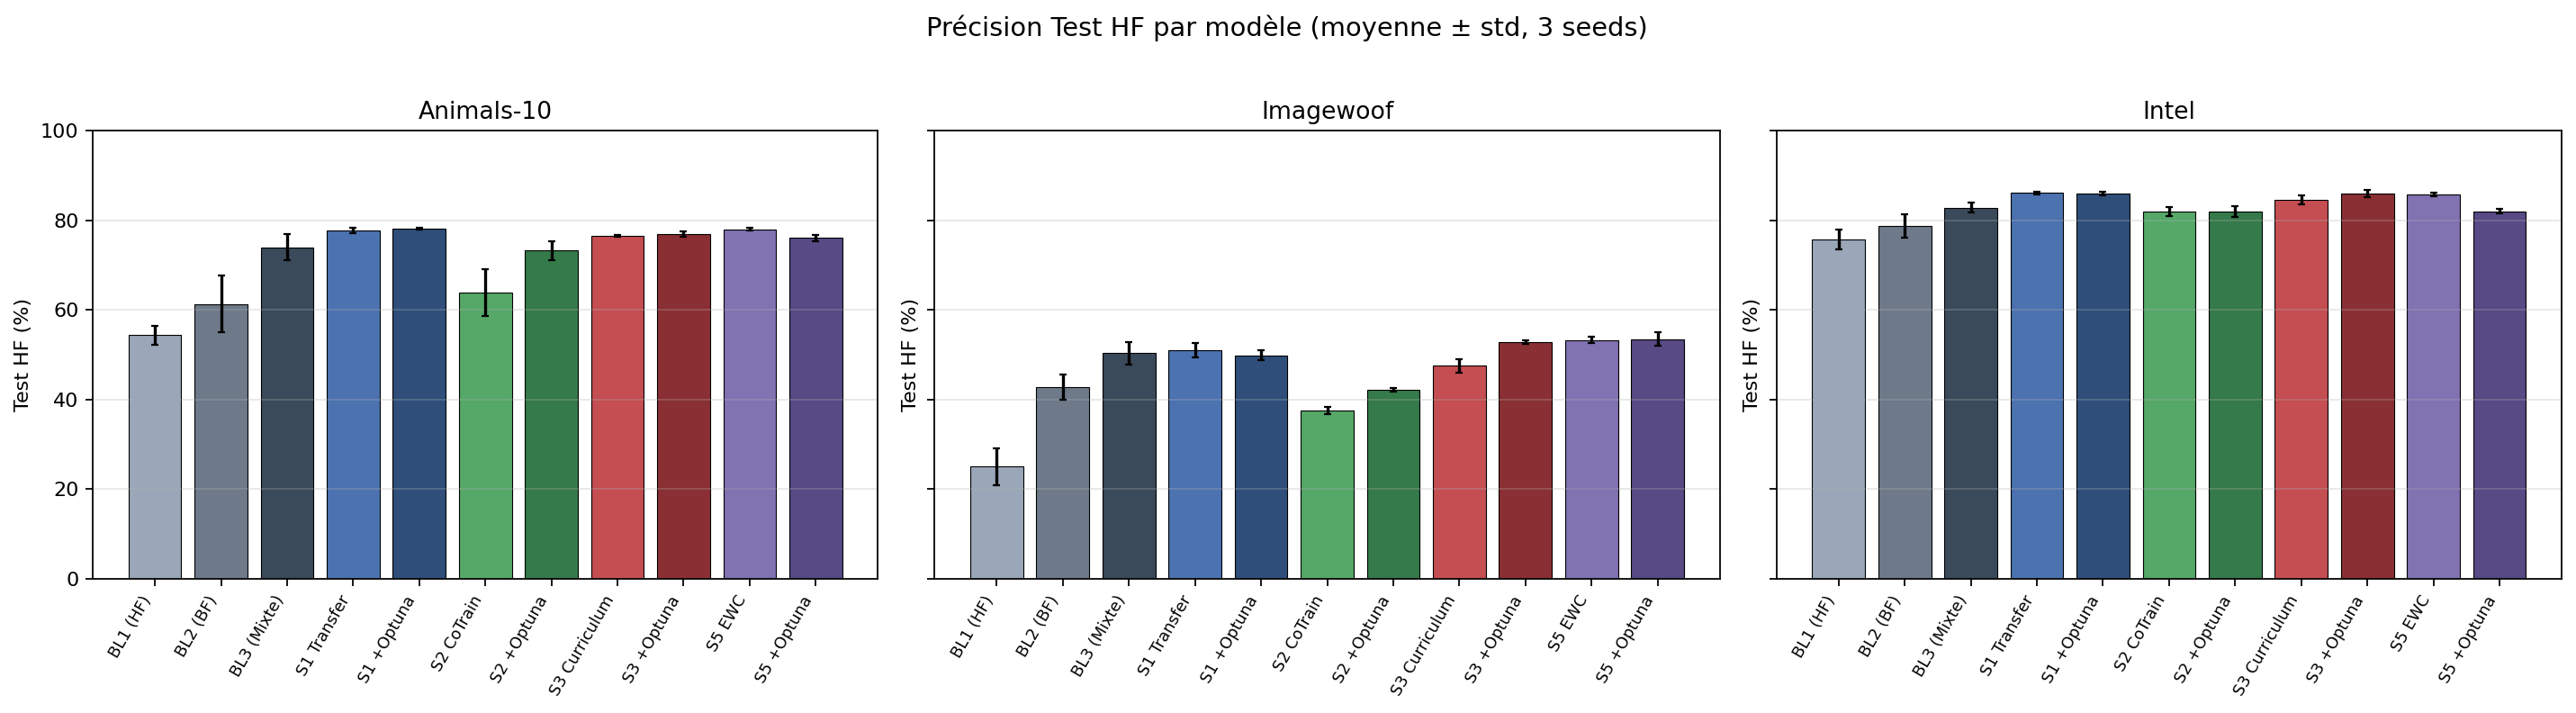
\includegraphics[width=\linewidth]{figures/hf_par_modele.png}
  \caption{Précision Test HF (moyenne $\pm$ écart-type) de tous les modèles, sur les trois datasets. (Légende : « S5 » = EWC = Stratégie 4 ; « S3 » = Curriculum = Stratégie 3.)}
  \label{fig:hf_par_modele}
\end{figure}

\section{Compromis coût / performance}

La figure de Pareto met en regard la précision HF et le coût. Les stratégies multi-fidélité forment la \textbf{frontière efficiente} : aucune baseline ne les domine simultanément en précision et en coût.

\begin{figure}[htbp]
  \centering
  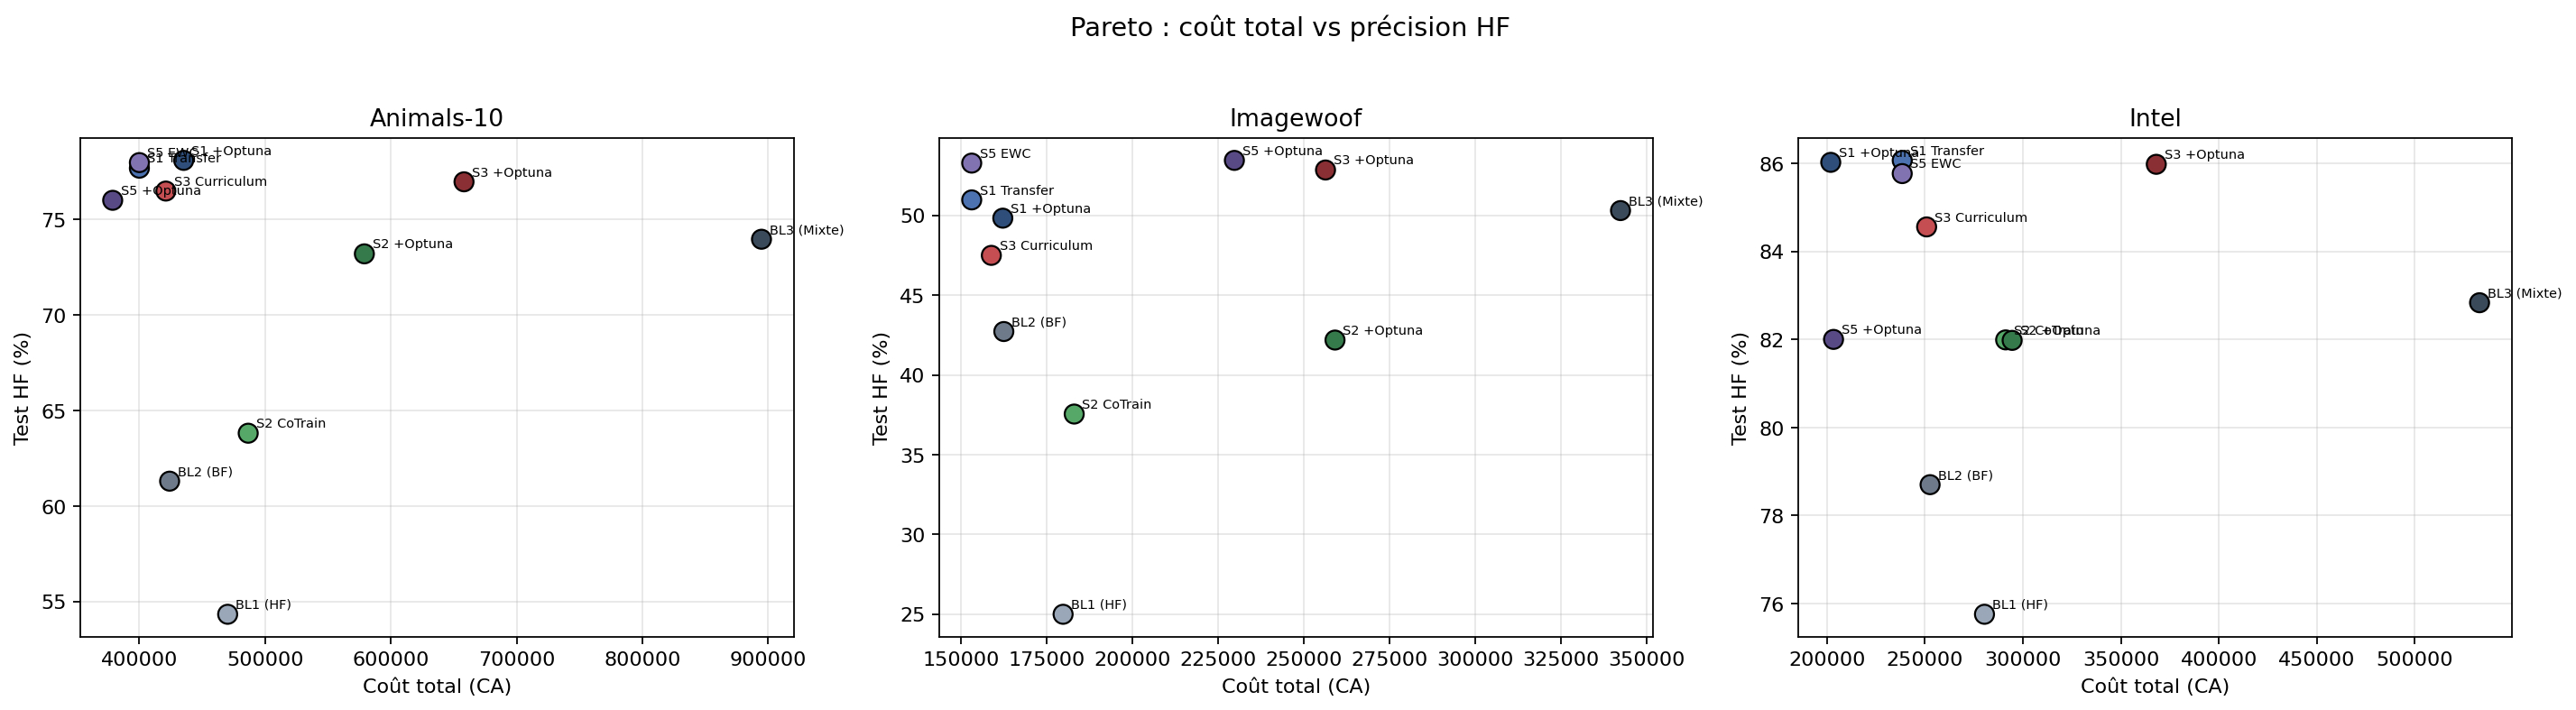
\includegraphics[width=\linewidth]{figures/pareto_cout_hf.png}
  \caption{Frontière de Pareto coût total vs précision Test HF. Les stratégies (haut-gauche : haute précision, faible coût) dominent les baselines.}
  \label{fig:pareto}
\end{figure}

\begin{figure}[htbp]
  \centering
  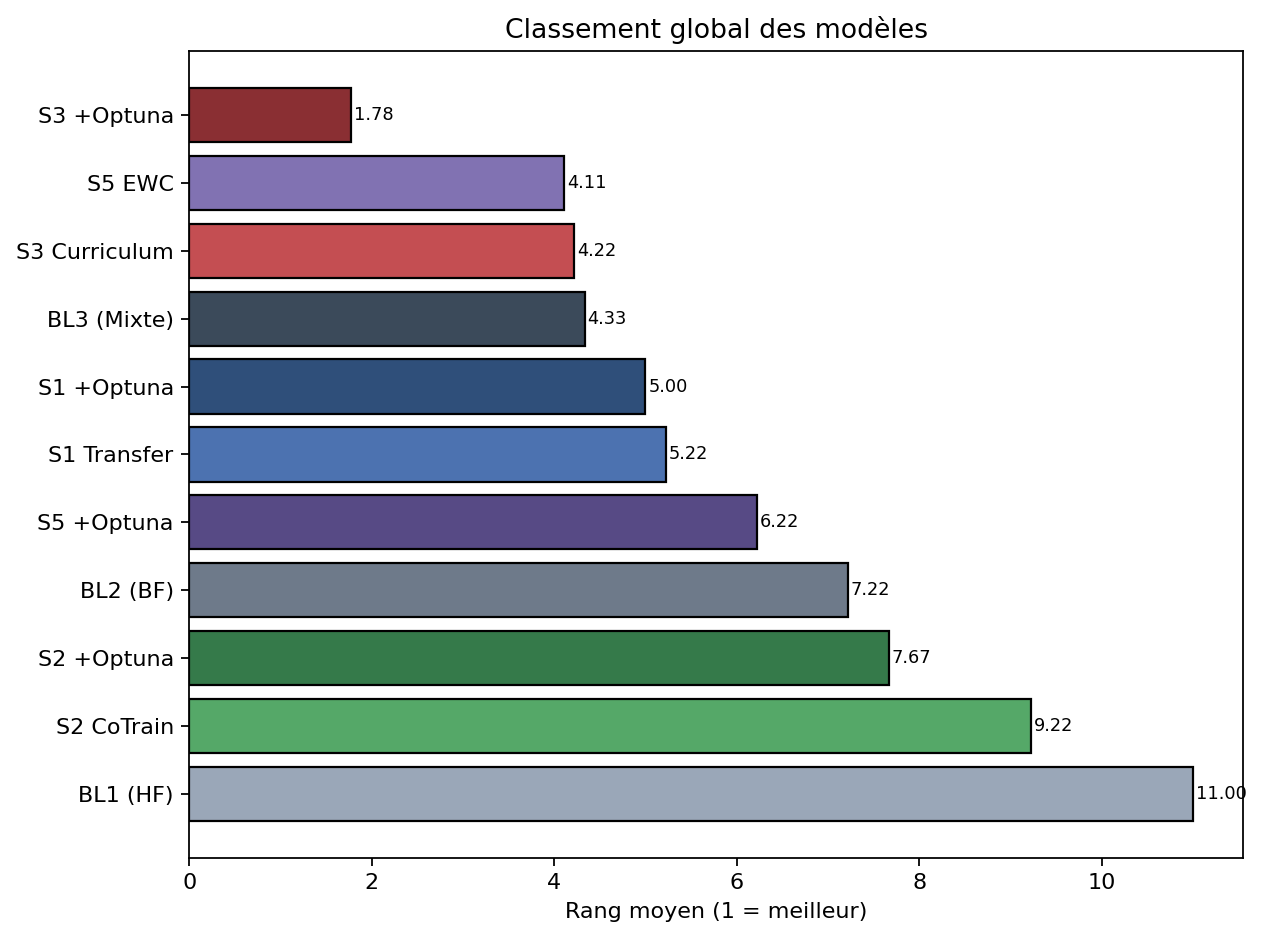
\includegraphics[width=\linewidth]{figures/classement_global.png}
  \caption{Classement global agrégé des modèles sur les trois datasets.}
  \label{fig:classement}
\end{figure}

\section{Robustesse des conclusions}

La force de ce travail tient à la \textbf{convergence des validations} :

\begin{itemize}
  \item \textbf{Multi-graines} : les conclusions reposent sur des moyennes $\pm$ écart-type (3 graines), écartant les artefacts d'initialisation ;
  \item \textbf{Triple dataset} : la hiérarchie se maintient sur des problèmes de volumes, granularités et natures différents (animaux, races fine-grained, scènes) ;
  \item \textbf{Analyses transversales} : robustesse à la dégradation et sensibilité au ratio de coût ont été examinées explicitement.
\end{itemize}

La principale nuance est que la \emph{hiérarchie d'efficience économique} dépend du ratio de coût supposé, alors que la \emph{hiérarchie de précision HF} est, elle, stable.


% ============================================================
%  CHAPITRE — Conclusion
% ============================================================
\chapter{Conclusion et perspectives}

\section{Bilan}

Ce travail a abordé une question concrète d'apprentissage multi-fidélité : \textbf{maximiser la performance sur données haute fidélité en exploitant un grand volume de données basse fidélité bon marché, au moindre coût}. Pour y répondre rigoureusement, un protocole reproductible a été construit — pipeline de dégradation déterministe, modèle de coût à trois métriques, trois modèles de référence — puis quatre stratégies multi-fidélité ont été développées, optimisées par Optuna, et validées sur trois datasets en multi-graines.

Les résultats sont clairs et convergents :

\begin{itemize}
  \item le \textbf{décalage de domaine} est réel et coûteux : un modèle Premium HF s'effondre face à des données dégradées ;
  \item le \textbf{paradoxe de la quantité} se vérifie : un grand volume BF bat un petit volume HF, même sur le test propre ;
  \item les \textbf{stratégies séquentielles guidées} (Transfer Learning et surtout \textbf{EWC}) atteignent la meilleure précision HF, dépassant le mélange naïf coûteux \textbf{tout en divisant le coût total par deux} ;
  \item le \textbf{Curriculum Learning} offre le meilleur compromis robustesse / équilibre HF-BF ;
  \item l'\textbf{objectif initial est atteint} : on obtient une performance supérieure à la borne haute pour un coût bien inférieur.
\end{itemize}

\section{Limites}

Plusieurs limites encadrent la portée de ces résultats : l'architecture est volontairement fixée (ResNet-18 \textit{from scratch}, sans pré-entraînement ImageNet) ; la dégradation BF, bien que réaliste, suit un schéma unique (sous-échantillonnage + bruit + JPEG) ; l'entraînement est borné à 20 époques et l'optimisation Optuna à 20 essais ; enfin, le jeu de données Food101 a dû être écarté pour des raisons techniques, limitant la validation à trois datasets.

\section{Perspectives}

Les pistes les plus prometteuses, détaillées par stratégie en \textbf{annexe}, sont :

\begin{itemize}
  \item \textbf{Backbones pré-entraînés} : initialiser depuis ImageNet ou comparer ResNet-34 / EfficientNet, à coût constant ;
  \item \textbf{Hybridation des stratégies} : combiner EWC \emph{et} curriculum (protéger les acquis BF \emph{pendant} une montée progressive en HF) pour viser à la fois précision et robustesse ;
  \item \textbf{Optimisation multi-objectif} : faire porter Optuna sur un compromis précision/coût, avec un budget d'essais accru ;
  \item \textbf{Early stopping et checkpointing} systématiques, pour gagner en stabilité ;
  \item \textbf{Élargissement} : davantage de datasets et de niveaux de fidélité (plusieurs intensités BF), et analyse par matrices de confusion pour comprendre les erreurs résiduelles.
\end{itemize}

En définitive, ce travail montre qu'avec une stratégie d'entraînement adaptée, \textbf{des données bon marché et imparfaites ne sont pas un pis-aller mais un véritable levier} : bien exploitées, elles permettent d'égaler, voire de surpasser, des approches bien plus coûteuses.


\newpage

\begin{thebibliography}{99}

% --- Architecture ---
\bibitem{resnet}
Kaiming He, Xiangyu Zhang, Shaoqing Ren, Jian Sun.
\textit{Deep Residual Learning for Image Recognition}.
Proceedings of the IEEE Conference on Computer Vision and Pattern Recognition (CVPR), 2016.

% --- Optimisation & entraînement ---
\bibitem{adam}
Diederik P. Kingma, Jimmy Ba.
\textit{Adam: A Method for Stochastic Optimization}.
International Conference on Learning Representations (ICLR), 2015.

\bibitem{crossentropy}
Ian Goodfellow, Yoshua Bengio, Aaron Courville.
\textit{Deep Learning}.
MIT Press, 2016.
Disponible en ligne : \url{https://www.deeplearningbook.org}

% --- Normalisation & transfert (ImageNet stats) ---
\bibitem{imagenet}
Olga Russakovsky, Jia Deng, Hao Su, Jonathan Krause, Sanjeev Satheesh, Sean Ma,
Zhiheng Huang, Andrej Karpathy, Aditya Khosla, Michael Bernstein, Alexander C. Berg, Li Fei-Fei.
\textit{ImageNet Large Scale Visual Recognition Challenge}.
International Journal of Computer Vision (IJCV), 123(3):211--252, 2015.

% --- Dégradation d'image & robustesse ---
\bibitem{hendrycks2019}
Dan Hendrycks, Thomas Dietterich.
\textit{Benchmarking Neural Network Robustness to Common Corruptions and Perturbations}.
International Conference on Learning Representations (ICLR), 2019.

% --- Multi-fidélité ---
\bibitem{multifidelity}
Marc Peter Deisenroth, Jun Wei Ng.
\textit{Distributed Gaussian Processes}.
International Conference on Machine Learning (ICML), 2015.

\bibitem{kennedy2000}
Marc C. Kennedy, Anthony O'Hagan.
\textit{Predicting the Output from a Complex Computer Code When Fast Approximations Are Available}.
Biometrika, 87(1):1--13, 2000.

% --- Méthodes de réentraînement robuste ---
\bibitem{ren2018reweight}
Mengye Ren, Wenyuan Zeng, Bin Yang, Raquel Urtasun.
\textit{Learning to Reweight Examples for Robust Deep Learning}.
International Conference on Machine Learning (ICML), 2018.

\bibitem{han2018coteaching}
Bo Han, Quanming Yao, Xingrui Yu, Gang Niu, Miao Xu, Weihua Hu, Ivor Tsang, Masashi Sugiyama.
\textit{Co-teaching: Robust Training of Deep Neural Networks with Extremely Noisy Labels}.
Advances in Neural Information Processing Systems (NeurIPS), 2018.

% --- Curriculum learning ---
\bibitem{bengio2009curriculum}
Yoshua Bengio, Jérôme Louradour, Ronan Collobert, Jason Weston.
\textit{Curriculum Learning}.
Proceedings of the 26th International Conference on Machine Learning (ICML), 2009.

% --- Apprentissage continu / oubli catastrophique (EWC) ---
\bibitem{kirkpatrick2017ewc}
James Kirkpatrick, Razvan Pascanu, Neil Rabinowitz, Joel Veness, Guillaume Desjardins, et al.
\textit{Overcoming Catastrophic Forgetting in Neural Networks}.
Proceedings of the National Academy of Sciences (PNAS), 114(13):3521--3526, 2017.

% --- Optimisation d'hyperparamètres ---
\bibitem{akiba2019optuna}
Takuya Akiba, Shotaro Sano, Toshihiko Yanase, Takeru Ohta, Masanori Koyama.
\textit{Optuna: A Next-generation Hyperparameter Optimization Framework}.
Proceedings of the 25th ACM SIGKDD International Conference on Knowledge Discovery \& Data Mining (KDD), 2019.

\end{thebibliography}

\appendix
\renewcommand{\thechapter}{\arabic{chapter}}
\setcounter{chapter}{0}

\chapter{Améliorations possibles des méthodes}

Cette annexe regroupe, pour chacune des quatre stratégies multi-fidélité, les leviers d'optimisation identifiés au fil de l'étude mais non explorés en dehors de l'optimisation Optuna. Ils constituent autant de pistes directes pour des travaux ultérieurs.

\section{Stratégie 1 — Transfer Learning séquentiel (BF $\rightarrow$ HF)}

Les résultats obtenus montrent que la stratégie séquentielle est déjà très compétitive sur HF, mais plusieurs leviers peuvent encore être optimisés.

\begin{itemize}
  \item \textbf{Nombre d'époques BF et HF} : modifier la durée relative pré-entraînement/fine-tuning (par ex. 5/15, 8/12, 12/8) peut déplacer le compromis robustesse BF vs spécialisation HF. \textit{Comment optimiser :} effectuer une recherche en grille sur le couple $(E_{BF}, E_{HF})$ et sélectionner la configuration maximisant Test HF.
  \item \textbf{Learning rates par phase} : un LR trop élevé en fine-tuning peut détruire des représentations utiles, trop faible peut sous-adapter HF. \textit{Comment optimiser :} tester plusieurs couples $(lr_{BF}, lr_{HF})$ avec schémas de décroissance (Cosine, StepLR, ReduceLROnPlateau).
  \item \textbf{Politique de gel/dégel des couches} : geler partiellement le backbone au début du fine-tuning peut limiter l'oubli BF tout en spécialisant la tête. \textit{Comment optimiser :} comparer \textit{full fine-tuning} vs \textit{head-only} puis dégel progressif bloc par bloc.
  \item \textbf{Split HF train/validation} : la proportion 80/20 peut être remplacée (70/30, 85/15) pour stabiliser la sélection de modèle. \textit{Comment optimiser :} valider sur plusieurs seeds et retenir la configuration la plus stable en variance de score HF.
  \item \textbf{Batch size} : influe sur la stabilité du gradient et la généralisation. \textit{Comment optimiser :} explorer 32/64/96 (selon VRAM) en ajustant le LR selon une règle de mise à l'échelle.
  \item \textbf{Régularisation} : ajouter \textit{weight decay}, \textit{dropout} ou \textit{label smoothing} peut réduire le sur-apprentissage en fin de phase HF. \textit{Comment optimiser :} balayage de plages courtes (ex. weight decay $\in [10^{-5},10^{-3}]$, label smoothing $\in [0.0,0.1]$).
  \item \textbf{Augmentations de données} : RandAugment, ColorJitter léger, RandomErasing peuvent améliorer la robustesse sans dégrader HF si bien dosés. \textit{Comment optimiser :} ablations une augmentation à la fois puis combinaison des plus bénéfiques.
  \item \textbf{Early stopping et checkpointing} : arrêter sur la meilleure validation HF évite la dégradation tardive. \textit{Comment optimiser :} utiliser une patience (3 à 5 époques) et conserver systématiquement le meilleur checkpoint HF.
  \item \textbf{Architecture backbone} : ResNet-18 est un bon compromis, mais ResNet-34 ou EfficientNet-B0 peuvent améliorer la représentation. \textit{Comment optimiser :} comparer à budget de coût constant et même protocole d'évaluation.
  \item \textbf{Fonction de coût avancée} : Focal Loss ou marges additives peuvent mieux séparer des classes ambiguës en HF. \textit{Comment optimiser :} tests contrôlés en remplaçant uniquement la loss, avec mêmes données et mêmes hyperparamètres de base.
\end{itemize}

\section{Stratégie 2 — Co-training pondéré (Reweighting)}

La stratégie de co-training pondéré offre une bonne robustesse inter-domaines ; son optimisation repose surtout sur le réglage fin du mélange de données et des poids de perte.

\begin{itemize}
  \item \textbf{Ratio HF/BF dans le batch} : le choix 16/48 (25\% HF) conditionne directement le compromis HF-BF. \textit{Comment optimiser :} tester plusieurs ratios (20/80, 30/70, 40/60) et tracer la frontière de Pareto entre Test HF et Test BF.
  \item \textbf{Poids de loss $w_{HF}$ et $w_{BF}$} : ce sont les hyperparamètres centraux de la méthode. \textit{Comment optimiser :} recherche en grille ou bayésienne sur $(w_{HF}, w_{BF})$ (ex. $w_{HF}\in[1.0,3.0]$, $w_{BF}\in[0.4,1.0]$), en fixant d'abord le ratio batch.
  \item \textbf{Planning dynamique des poids} : garder des poids constants peut être sous-optimal selon la phase d'apprentissage. \textit{Comment optimiser :} démarrer avec un poids HF modéré puis l'augmenter progressivement (curriculum de pondération).
  \item \textbf{Nombre d'époques} : des oscillations de validation suggèrent qu'un arrêt plus précoce peut être préférable à 20 époques fixes. \textit{Comment optimiser :} early stopping sur validation HF avec patience et sauvegarde du meilleur modèle.
  \item \textbf{Learning rate et scheduler} : un LR fixe peut accentuer l'instabilité tardive. \textit{Comment optimiser :} comparer LR fixes vs Cosine Annealing / OneCycleLR pour lisser la convergence.
  \item \textbf{Composition des batches (stochastique contrôlée)} : la variabilité intra-batch peut influencer la stabilité. \textit{Comment optimiser :} conserver le ratio global mais imposer une diversité de classes par domaine (batch balancing par classe).
  \item \textbf{Fonction de loss alternative} : Balanced Softmax, focal reweighting, ou class-balanced loss peuvent mieux traiter classes rares et bruitées. \textit{Comment optimiser :} protocole d'ablation en ne changeant qu'une composante de loss à la fois.
  \item \textbf{Qualité de la dégradation BF} : le niveau de bruit/sous-échantillonnage détermine l'écart de domaine. \textit{Comment optimiser :} calibrer plusieurs intensités de dégradation puis choisir celle qui maximise la généralisation HF sans effondrer BF.
  \item \textbf{Régularisation et normalisation} : weight decay, EMA des poids, mixup/cutmix peuvent améliorer la robustesse de l'entraînement mixte. \textit{Comment optimiser :} introduire les techniques progressivement et évaluer le gain marginal.
  \item \textbf{Validation multi-critères} : optimiser uniquement HF peut dégrader excessivement BF. \textit{Comment optimiser :} utiliser un score composé (ex. $S=\alpha\,Acc_{HF}+(1-\alpha)\,Acc_{BF}$) avec $\alpha$ élevé, cohérent avec la priorité HF.
\end{itemize}

\section{Stratégie 3 — Curriculum Learning progressif}

\begin{itemize}
  \item \textbf{Planning des paliers} : le découpage 0/25/60/100 \% peut être affiné. \textit{Comment optimiser :} rechercher le nombre de paliers, leur durée et les proportions HF (lissage continu plutôt que paliers, fonctions de montée linéaire/exponentielle).
  \item \textbf{Durée de la phase finale HF} : un dernier palier 100 \% HF plus long rapprocherait le modèle d'un fine-tuning dédié. \textit{Comment optimiser :} balayer la longueur du dernier palier en surveillant le compromis HF/BF.
  \item \textbf{Learning rate par palier} : un LR décroissant à chaque montée en HF stabiliserait la transition. \textit{Comment optimiser :} associer un scheduler (Cosine, StepLR) au planning de curriculum.
  \item \textbf{Critère d'avancement adaptatif} : passer au palier suivant non pas à époque fixe mais selon la convergence. \textit{Comment optimiser :} déclencher la montée en HF lorsque la validation plafonne (curriculum auto-pacé).
  \item \textbf{Régularisation} : weight decay / label smoothing pour réduire le sur-apprentissage de la phase HF finale. \textit{Comment optimiser :} balayage court de ces hyperparamètres.
\end{itemize}

\section{Stratégie 4 — Elastic Weight Consolidation (EWC)}

\begin{itemize}
  \item \textbf{Force du rappel ($\lambda$)} : hyperparamètre central. \textit{Comment optimiser :} balayer $\lambda$ (ex. $[10, 1000]$ en échelle log) et tracer le compromis HF/BF résultant.
  \item \textbf{Estimation de Fisher} : 1\,000 échantillons est un compromis. \textit{Comment optimiser :} faire varier le nombre d'échantillons et comparer Fisher diagonale vs approximations plus riches.
  \item \textbf{EWC en ligne / multi-tâches} : accumuler l'importance sur plusieurs domaines (BF de différentes intensités). \textit{Comment optimiser :} EWC en ligne (online EWC) avec mise à jour incrémentale de $F$.
  \item \textbf{Couplage avec le curriculum} : appliquer EWC \emph{pendant} une montée progressive en HF. \textit{Comment optimiser :} combiner planning de curriculum et pénalité de Fisher, puis mesurer le gain conjoint.
  \item \textbf{Learning rate de fine-tuning} : interagit fortement avec $\lambda$. \textit{Comment optimiser :} recherche conjointe $(\lambda, lr_{HF})$ plutôt que séparée.
\end{itemize}


\end{document}
